\documentclass{LS}
\usepackage{multicol}
\usepackage[numbers]{natbib}
\usepackage{url}
\usepackage{graphicx}
\usepackage{caption}
\usepackage{amsmath}
\usepackage{subcaption}
\usepackage{multirow}
\usepackage{booktabs}
\usepackage{float} 
\usepackage{algorithm}
\usepackage{algorithmic}
\usepackage{colortbl}
\usepackage{longtable}
\usepackage{geometry}
\usepackage{array}
\usepackage{tabularx} 
\usepackage{tocloft}
\usepackage{pgfgantt}
\usepackage{hyperref}
\usepackage{tikz}
\usepackage[numbers]{natbib}
\usepackage{xcolor}
\floatname{algorithm}{}





% Definiciones para el índice de ecuaciones
\newcommand{\listequationsname}{Índice de Ecuaciones}
\newlistof{myequations}{loe}{\listequationsname}

% Title

\title{\LARGE[TG253015 ] Desarrollo tecnológico de un motor rotativo Wankel de 6 tiempos mediante la modelación termo - mecánica de su funcionamiento}

% Authors
\author{
    Juan José Rojas Barón\textsuperscript{a,d},
    Vanessa María Serpa Páez\textsuperscript{a,d},\\
    Camilo Andres Bayona Roa\textsuperscript{b,d},
    
}


\begin{document}
\maketitle

\noindent\hrulefill
\vspace{-1em} 
\begin{abstract}
This project addresses the low thermal efficiency and high unburned hydrocarbon (uHC) emissions typical of conventional Wankel engines by proposing a six-stroke rotary design capable of performing a second controlled combustion. The proposed configuration includes two geometric variants—three-lobe/four-side and four-lobe/five-side rotors—whose epitrochoidal relations were modeled and simulated through a computational tool developed entirely in Python. The simulation integrates geometric and thermodynamic formulations to solve polytropic and isochoric processes, obtaining instantaneous pressure, temperature, torque, and power profiles for each case. Verification was conducted through mass and energy balances, ensuring numerical stability and coherence under cloud-based computation constraints. The six-stroke engine with an expansion valve achieved the highest thermal efficiency (68.3\%), followed by the supercharged (50.9\%) and water-injection (44.4\%) configurations, all surpassing the conventional four-stroke engine (30.9\%). The design meets the performance requirements established for thermal engines and demonstrates the feasibility of a cleaner, more efficient rotary architecture capable of recovering residual energy through secondary combustion.
\end{abstract}


\vspace{-1em} 

\begin{center}
\textbf{\textit{\fontsize{8}{10}\selectfont Keywords:}} \textit{\fontsize{8}{10}\selectfont   Motor Wankel, seis tiempos, combustión secundaria, hidrocarburos no quemados (uHC), eficiencia térmica, simulación computacional, modelado termo-mecánico. }
\end{center}

\noindent\hrulefill

% Main Content

\section{\bfseries\fontsize{10}{12}\selectfont Planteamiento del problema y Justificación del Proyecto }\label{sec:intro}

La humanidad enfrenta actualmente el reto de transformar y utilizar la energía de forma más eficiente y sostenible. La demanda energética mundial ha aumentado de manera sostenida debido al crecimiento poblacional, la digitalización y la electrificación de procesos, alcanzando un incremento del 2.2\% solo en 2024, impulsado principalmente por el sector eléctrico, que creció un 4.3\% de acuerdo con \cite{iea2025a,iea2025b}. Este consumo intensivo, todavía dominado por los combustibles fósiles, es responsable de aproximadamente el 42\% de las emisiones globales de gases de efecto invernadero según \cite{ipcc2022a,ipcc2022b}. Frente a este panorama, la transición energética se ha convertido en un imperativo técnico y ético, impulsando el desarrollo de nuevas tecnologías que logren una conversión energética más eficiente como lo mencionan \cite{perino2021}.

Entre las tecnologías de conversión energética, los motores de combustión interna siguen teniendo una participación considerable a nivel global. En 2023, los combustibles fósiles representaron aproximadamente el 80\% de la demanda energética mundial, lo que refleja el papel predominante que aún juegan los motores térmicos en el transporte y la industria de acuerdo con \cite{iea2024}. En este contexto, el motor rotativo Wankel destaca por su alta densidad de potencia, diseño compacto, menor número de partes móviles y operación suave. Según \cite{cole1972}, el motor Wankel presenta la ventaja de realizar de forma simultánea tres fases diferentes del ciclo termodinámico: admisión, compresión y expansión, en sus respectivas cámaras, lo que contribuye a una entrega de potencia más fluida y constante, además de operar con menos fricción y menor peso. En la figura 1 se describen los componentes principales del motor Wankel de cuatro tiempos, así como su funcionamiento.

\begin{figure}[H]
    \centering
    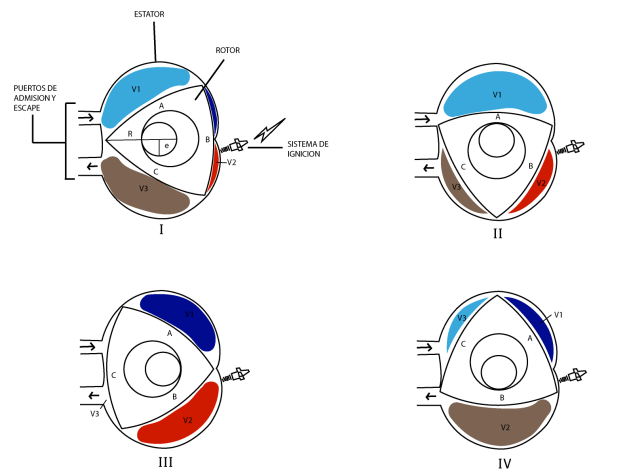
\includegraphics[width=0.4\textwidth]{imagenes/Wankel.png}
    \caption{Ciclo básico de funcionamiento del motor Wankel de cuatro tiempos. Tomado de \cite{canals2011}, p. 9.}
    \label{fig:geometria-yamamoto}
\end{figure}


Sin embargo, una de las particularidades más críticas del diseño del motor Wankel es la necesidad de inyectar aceite directamente en la cámara de combustión para lubricar los sellos del rotor, lo cual genera un consumo de aceite significativamente más alto en comparación con los motores de pistones \cite{elbahja2023}. Esta característica de diseño, junto con otros desafíos técnicos, ha limitado históricamente su aplicación. Entre estos se destacan su baja eficiencia térmica, las elevadas emisiones de hidrocarburos no quemados (uHC) y el ya mencionado consumo elevado de aceite.

En un estudio comparativo entre un motor rotativo Mazda 13B de 1308 cm\textsuperscript{3} y un motor de pistones Buick V6 de 3777 cm\textsuperscript{3}, ambos con potencias similares, \cite{cole1976} encontraron que el motor Wankel presentaba emisiones de hidrocarburos entre 6 y 10 veces superiores. Estas deficiencias fueron atribuidas a la geometría alargada de la cámara de combustión, particularmente por su alta relación superficie-volumen y la dificultad de acceso de la llama a ciertas zonas de la mezcla, lo que favorece una combustión incompleta y, por consiguiente, un aumento significativo en la generación de hidrocarburos no quemados de acuerdo con \cite{yamamoto1972}.


De acuerdo con \cite{kuppa2019}, en motores de pistones los uHC generados por crevices pueden alcanzar concentraciones de hasta 1100 ppm, y los causados por el apagamiento de llama en la pared hasta 600 ppm, dando un total aproximado de 1700 ppm. Considerando la proporción reportada por \cite{cole1976}, según la cual los motores Wankel emiten entre 6 y 10 veces más uHC, se puede estimar que estos podrían alcanzar concentraciones entre 10200 ppm y 17\,000 ppm. Complementariamente, un estudio realizado por la NASA comparó motores Wankel con motores de pistones de aviación bajo condiciones operativas equivalentes, y halló que el consumo específico de combustible al freno (BSFC) del motor rotativo fue entre un 15\% y 20\% más alto, reflejando una conversión menos eficiente de la energía del combustible en trabajo útil \cite{nasa1984}.

Este conjunto de limitaciones ambientales y energéticas evidencia que una fracción considerable del combustible permanece sin oxidar al finalizar la combustión primaria, lo que representa simultáneamente una pérdida de eficiencia y un impacto ambiental significativo. A partir de esta problemática surge la motivación principal del presente proyecto: explorar una estrategia que permita aprovechar energéticamente los hidrocarburos no quemados (uHC) y el calor residual de los gases retenidos en la cámara, mediante la incorporación de una segunda combustión controlada. El propósito es recuperar parte de la energía que actualmente se pierde, generando trabajo adicional sin necesidad de introducir más combustible y contribuyendo a mitigar las emisiones características del motor Wankel.

En este contexto, emergen propuestas de rediseño del ciclo termodinámico convencional de cuatro tiempos, como el motor Wankel de seis tiempos, que incorpora etapas adicionales de admisión y expansión. Su desarrollo requiere herramientas de simulación adaptadas a un comportamiento no convencional, tanto en la dinámica de volúmenes como en el tratamiento de la combustión residual. Esta idea se fundamenta en el análisis geométrico realizado por Yamamoto en su obra \textit{Rotary Engine}, donde se documentan variaciones sobre la curva epitrocoidal que constituye la base del motor Wankel de cuatro tiempos, incluyendo la factibilidad de incorporar tiempos adicionales. En la Figura 2 se observa la geometría del motor Wankel de cuatro tiempos (2) y la geometría que cumple con las condiciones para llevar a cabo los seis tiempos (3).


\begin{figure}[H]
    \centering
    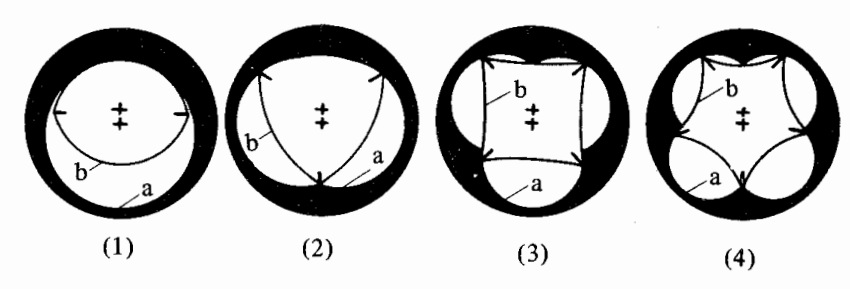
\includegraphics[width=0.4\textwidth]{imagenes/4 y 6.png}
    \caption{Comparación de variaciones geométricas en el diseño del motor Wankel. Tomado de \textcite{yamamoto1971}, p. 9.}
    \label{fig:geometria-yamamoto}
\end{figure}

Actualmente, no existen motores rotativos Wankel de seis tiempos con una segunda fase de combustión para el aprovechamiento de los uHC desarrollados ni documentados en la literatura, lo que convierte esta configuración en una propuesta completamente original. A su vez, tampoco se dispone de herramientas computacionales ni modelos termodinámicos generalizados que permitan analizar, simular u optimizar el comportamiento de este tipo de arquitectura extendida, lo cual representa una barrera técnica significativa y una brecha relevante en la investigación actual.

La ejecución de este proyecto tiene implicaciones significativas tanto en el ámbito teórico como en aplicaciones reales. Desde la perspectiva académica, el desarrollo de una herramienta computacional para modelar un motor Wankel de seis tiempos representa un aporte inédito, al proponer un marco de simulación adaptable a configuraciones rotativas no convencionales. Esta herramienta permitirá analizar fenómenos asociados a la termodinámica de doble combustión, evaluar diferentes geometrías y optimizar el desempeño del ciclo, abriendo nuevas líneas de investigación en el campo de las máquinas térmicas. En el plano práctico, el diseño propuesto puede aplicarse en escenarios donde el espacio, el peso y la eficiencia energética son factores críticos, como en sistemas de movilidad eléctrica, generadores compactos o vehículos aéreos no tripulados. En la actualidad, los motores Wankel se emplean en diversas tecnologías gracias a su compacidad, bajo peso y elevada densidad de potencia. Un ejemplo es el Mazda MX-30 e-Skyactiv R-EV, que incorpora un motor rotativo como generador para recargar baterías, combinando la eficiencia de la propulsión eléctrica con la versatilidad térmica \cite{mazda2023}. En el ámbito militar, la empresa AIE ha desarrollado el motor rotativo 225CS para UAVs, con capacidad multifuel y alta relación potencia-peso \cite{aie2024}. Por su parte, la compañía LiquidPiston diseñó el motor X Mini, de 70 cc, destacando por su eficiencia energética, compacidad y capacidad para operar con distintos combustibles, siendo ideal para generadores portátiles y vehículos ligeros \cite{liquidpiston2024}.
}.

En este contexto, el desarrollo de un motor Wankel de seis tiempos otorgaría mejoras que serían especialmente valiosas en las aplicaciones mencionadas, donde el espacio y la autonomía energética son críticos, posicionando a esta arquitectura como una alternativa prometedora para la siguiente generación de tecnologías compactas, híbridas o portátiles. Así, el proyecto no solo busca resolver una necesidad técnica no atendida, sino también abrir el camino hacia soluciones energéticas más  eficientes y adaptables a contextos tecnológicos emergentes.



\section{\bfseries\fontsize{10}{12}\selectfont Antecedentes} \label{sec:intro} 

Desde tiempos antiguos, la humanidad ha buscado transformar la energía natural de manera más eficiente, comenzando con la fuerza humana y animal, y luego aprovechando fuentes como el viento y el agua mediante dispositivos como molinos y norias \cite{pacheco2015, kandari2013}. La invención de la máquina de vapor en el siglo XVIII permitió convertir calor en trabajo mecánico continuo, impulsando la Revolución Industrial y el uso intensivo de combustibles fósiles \cite{pacheco2015}. Posteriormente, en el siglo XIX, surgieron los motores de combustión interna, que transforman la energía química de los combustibles en movimiento rotativo, sentando las bases de la ingeniería energética moderna \cite{morocho2023}. Estos motores se han consolidado en transporte, industria y generación eléctrica, con mejoras continuas en eficiencia y emisiones. Los motores Otto y Diesel alcanzan eficiencias ideales de 25–30\% y hasta 45\%, respectivamente \cite{guzzella2010, olivier2021}}.

Desde su invención, los motores de combustión interna han evolucionado principalmente en configuraciones de dos y cuatro tiempos, ampliamente utilizadas en aplicaciones móviles e industriales. El motor de dos tiempos completa un ciclo de admisión, compresión, combustión y escape en una sola vuelta del cigüeñal, lo que le permite generar más potencia por unidad de volumen. Específicamente, estos motores pueden producir aproximadamente un 17\,\% más de potencia en comparación con motores de cuatro tiempos de tamaño similar acorde con lo que menciona \cite{amet2002}. Sin embargo, esta mayor potencia conlleva desventajas significativas: los motores de dos tiempos suelen consumir más combustible y emitir mayores niveles de contaminantes. De hecho, se ha observado que las emisiones de hidrocarburos en motores de dos tiempos pueden ser hasta seis veces superiores a las de motores de cuatro tiempos  según \cite{downtoearth2001}.

\begin{figure}[H]
    \centering
    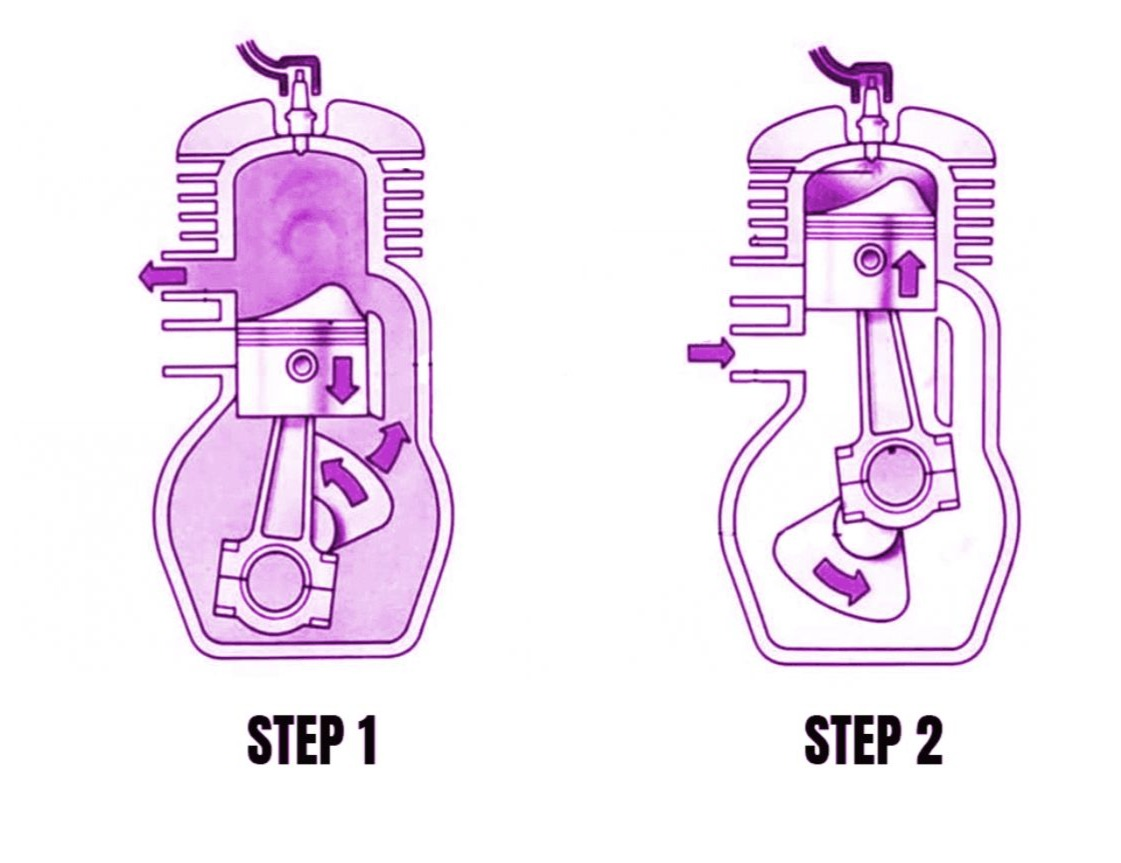
\includegraphics[width=0.3\textwidth]{imagenes/2tiempos.jpg}
    \caption{Ciclo básico de funcionamiento del motor de dos tiempos. Tomado de \cite{jcosta2t}}
    \label{fig:2tiempos}
\end{figure}

Por otro lado, el motor de cuatro tiempos distribuye las fases de admisión, compresión, combustión y escape en dos vueltas completas del cigüeñal. Esta configuración mejora la eficiencia térmica y reduce las emisiones contaminantes. Estudios indican que los motores de cuatro tiempos pueden ser hasta un 50\,\% más eficientes en el consumo de combustible que sus contrapartes de dos tiempos de acuerdo con \cite{boatersworld2023}. Además, las emisiones de hidrocarburos en motores de cuatro tiempos son significativamente menores, representando solo una fracción de las emitidas por motores de dos tiempos de acuerdo con \cite{downtoearth2001}.

\begin{figure}[H]
    \centering
    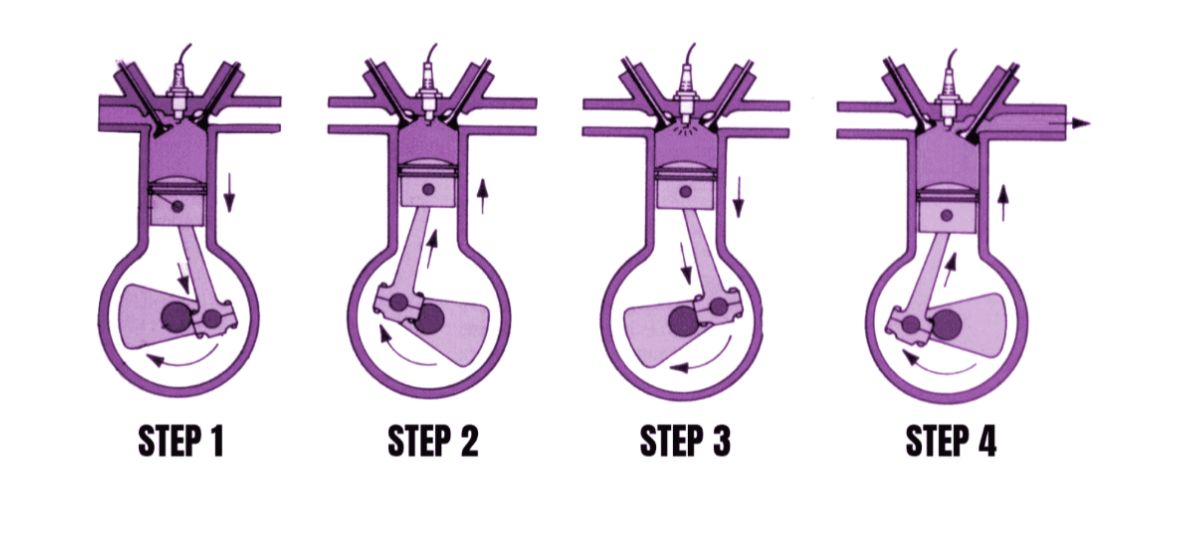
\includegraphics[width=0.5\textwidth]{imagenes/4tiempos.jpg}
    \caption{Ciclo básico de funcionamiento del motor de cuatro tiempos. Tomado de \cite{jcosta4t}}
    \label{fig:4tiempos}
\end{figure}

Ambos tipos de motores presentan una sola combustión por ciclo y una única expansión del gas, lo que limita el aprovechamiento energético total como lo menciona \cite{fiveable2023}. Estas limitaciones justifican la aparición de configuraciones extendidas como los motores de seis tiempos, que permiten incorporar etapas adicionales para recuperar calor o limpiar la cámara de combustión, aumentando así la eficiencia global del ciclo de acuerdo con \cite{kandari2013, bajulaz1989}.

El motor de seis tiempos desarrollado por Roger Bajulaz en 1989 introduce dos etapas adicionales al ciclo convencional de cuatro tiempos: una segunda expansión y un segundo escape. Tras la fase de escape tradicional, se inyecta agua fría en la cámara de combustión caliente. Esta agua se vaporiza instantáneamente debido al calor residual, generando una expansión adicional que produce trabajo útil sin consumo extra de combustible. Este proceso no solo mejora la eficiencia térmica del motor, sino que también contribuye a la reducción de la temperatura de operación y de las emisiones contaminantes. Estudios indican que la inyección de agua en motores de seis tiempos puede reducir la temperatura de la culata hasta en un 50\%, lo que disminuye la necesidad de sistemas de enfriamiento convencionales. Además, se ha observado una disminución en el consumo de combustible de al menos un 40\% y una reducción significativa en las emisiones de óxidos de nitrógeno (NOx) y otros contaminantes como se menciona en \cite{review2017}.

\begin{figure}[H]
    \centering
    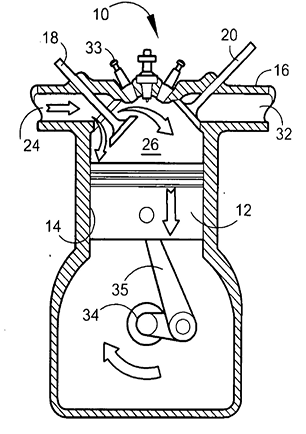
\includegraphics[width=0.2\textwidth]{imagenes/bajulaz.png}
    \caption{Motor Bajulaz de seis tiempos. Tomado de \cite{bajulaz1989}}
    \label{fig:bajulaz}
\end{figure}

El motor Velozeta, por su parte, añade dos fases adicionales orientadas a limpieza y enfriamiento del cilindro. Tras la combustión y escape tradicionales, el motor introduce una fase de barrido con aire comprimido, y luego una fase de refrigeración, también con aire, antes de repetir el ciclo. Estas etapas estabilizan térmicamente el sistema, aunque no generan trabajo adicional como en el caso de Bajulaz de acuerdo con \cite{pande2015}.

\begin{figure}[H]
    \centering
    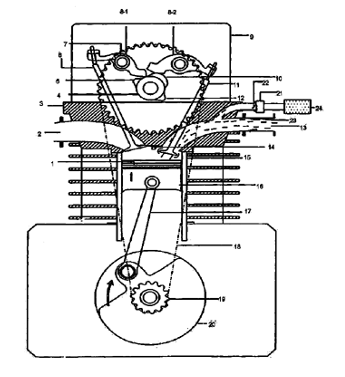
\includegraphics[width=0.23\textwidth]{imagenes/velozeta.png}
    \caption{Motor Velozeta de seis tiempos. Tomado de \cite{pande2015}}
    \label{fig:velozeta}
\end{figure}

En 2024, Porsche patentó un motor de seis tiempos que introduce un sistema de excentricidad en el cigüeñal, permitiendo al pistón alcanzar dos puntos muertos inferiores distintos durante el ciclo. Esta geometría habilita una segunda compresión tras la fase de escape, mediante la admisión de aire fresco a través de puertos laterales, justo cuando el pistón llega al punto más bajo. Esta segunda mezcla se combina con los hidrocarburos no quemados (uHC) de la combustión anterior, permitiendo una nueva ignición sin inyección adicional de combustible según \cite{porsche2024}.

\begin{figure}[H]
    \centering
    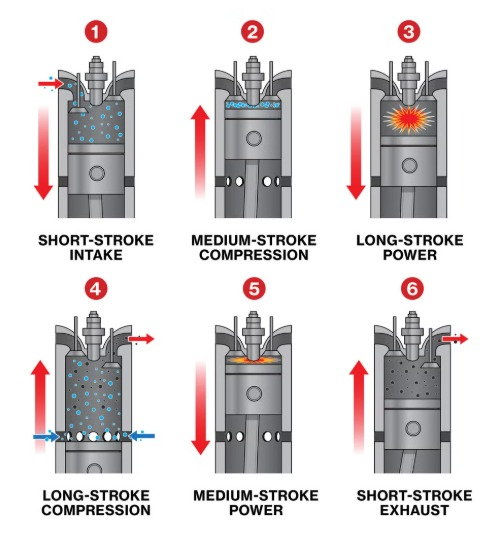
\includegraphics[width=0.3\textwidth]{imagenes/porshe.jpg}
    \caption{Motor Porsche de seis tiempos. Tomado de \cite{porsche2024}}
    \label{fig:porsche}
\end{figure}

El motor X desarrollado por LiquidPiston implementa el ciclo híbrido de alta eficiencia (HEHC), combinando elementos de los ciclos Otto, Diesel y Atkinson. Este motor rotativo presenta un rotor con forma de lóbulos que gira dentro de una carcasa triangular fija, realizando los procesos de admisión, compresión, combustión y escape en tres cámaras separadas. Una característica destacada del motor X es su capacidad para operar con una relación de compresión elevada. En los prototipos de encendido por compresión (CI-HEHC), se han alcanzado relaciones de compresión de hasta 26:1, lo que mejora significativamente la eficiencia térmica del motor de acuerdo con \cite{liquidpiston2023}. Además, el diseño del motor permite una combustión cercana a condiciones de volumen constante. Esto se logra mediante una detención cerca del punto muerto superior, que prolonga el tiempo disponible para la combustión. Esta característica, junto con la alta relación de compresión, contribuye a una mejor gestión térmica y a una reducción en el tiempo de combustión, optimizando el rendimiento del motor de acuerdo con \cite{liquidpiston2023}.

\begin{figure}[H]
    \centering
    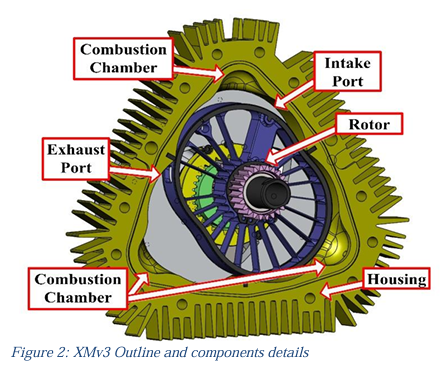
\includegraphics[width=0.3\textwidth]{imagenes/liquid.png}
    \caption{Motor LiquidPiston XMv3. Tomado de \cite{liquidpiston2015}}
    \label{fig:liquidpiston}
\end{figure}

El segundo caso son los motores \textit{rotary vane} o de paletas rotativas. En estos diseños, un rotor central gira dentro de una carcasa con forma excéntrica y posee varias paletas móviles que se expanden radialmente hacia las paredes internas de la carcasa. Estas paletas dividen el espacio en múltiples cámaras de trabajo que varían de volumen a medida que el rotor gira, permitiendo realizar de forma continua las etapas del ciclo: admisión, compresión, combustión y escape. Su diseño compacto, con pocas piezas móviles—generalmente cuatro: el rotor, la carcasa y dos paletas deslizantes como lo menciona \cite{csef2012} y rotación continua, proporciona una entrega de energía estable y un potencial de alto rendimiento volumétrico. Sin embargo, enfrentan desafíos de sellado dinámico, especialmente en las paletas, así como problemas de desgaste y eficiencia térmica a altas cargas como lo menciona \cite{sharma2017}. Recientemente, se ha patentado un diseño de motor rotary vane de seis tiempos, el cual añade dos etapas adicionales de expansión y escape. El sistema cuenta con cámaras distribuidas alrededor del rotor que permiten gestionar por separado la primera y segunda combustión, así como los gases residuales. Las válvulas de control y las geometrías internas están diseñadas para secuenciar los seis tiempos sin interrupción del giro de acuerdo con \cite{vane6t2022}.

\begin{figure}[H]
    \centering
    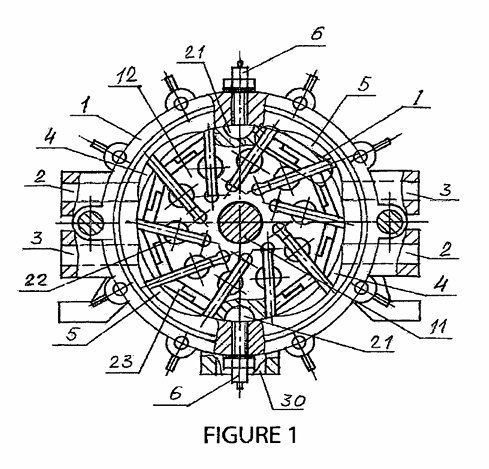
\includegraphics[width=0.3\textwidth]{imagenes/vane6.png}
    \caption{Motor Rotary Vane de seis tiempos. Tomado de \cite{vane6t2022}}
    \label{fig:vane}
\end{figure}

A diferencia de estos desarrollos, la presente propuesta plantea un motor rotativo tipo Wankel con seis tiempos, que conserva la arquitectura rotativa original pero añade una segunda fase de admisión, compresión y combustión. Esto permitiría reaprovechar los hidrocarburos no quemados (uHC) de la primera combustión, generando una nueva ignición sin añadir combustible adicional, lo cual no ha sido documentado ni implementado en configuraciones rotativas actuales, y además, no existen modelos computacionales que permitan simular este tipo de arquitectura extendida. Así, este proyecto aborda una brecha tecnológica real en el desarrollo de motores rotativos de múltiples tiempos, al tiempo que propone una nueva herramienta de modelado computacional adaptada a esta arquitectura no convencional.


\section{\bfseries\fontsize{10}{12}\selectfont Objetivos }\label{sec:intro}

\textit{Desarrollar una herramienta computacional que permita modelar el comportamiento termomecánico de un motor rotativo tipo Wankel de seis tiempos, mediante la formulación de modelos numéricos, así como su codificación en lenguajes de programación} para apoyar tareas de diseño mediante la variación de parámetros geométricos.

\begin{enumerate}
    \item Definir la arquitectura del motor Wankel de seis tiempos y caracterizar sus relaciones geométricas para representar el ciclo completo.

    \item Formular un modelo matemático que represente el comportamiento termo-mecánico del motor Wankel, considerando los procesos de admisión, compresión, combustión, expansión, postcompresión, postcombustión y postexpansión.

    \item Implementar el modelo en una herramienta computacional desarrollada en lenguajes de programación de alto nivel, para simular el comportamiento del motor bajo distintas condiciones geométricas.

    \item Comparar el desempeño del motor Wankel de seis tiempos frente a un modelo convencional de cuatro tiempos.
\end{enumerate}


\subsection{Desarrollo conceptual de las fases operativas del ciclo Wankel de seis tiempos}

A partir de los antecedentes de motores de seis tiempos con inyección de agua \cite{bajulaz1989} y del diseño de Porsche con doble admisión y escape \cite{porsche2024}, se concluye que la viabilidad del ciclo Otto modificado en arquitectura rotativa depende de la tríada: geometría del estator, número de caras del rotor y relación de giro eje–rotor. El análisis del orden de los tiempos y de las exigencias termodinámicas llevó a dos configuraciones funcionales para un Wankel: (i) estator de tres lóbulos con rotor de cuatro lados (4:1), y (ii) estator de cuatro lóbulos con rotor de cinco lados (5:1), mostradas en las Figuras~\ref{fig:camara-3lob} y~\ref{fig:camara-4lob}.


 

\begin{figure}[H]
  \centering
  \begin{subfigure}[t]{0.48\textwidth}
    \centering
    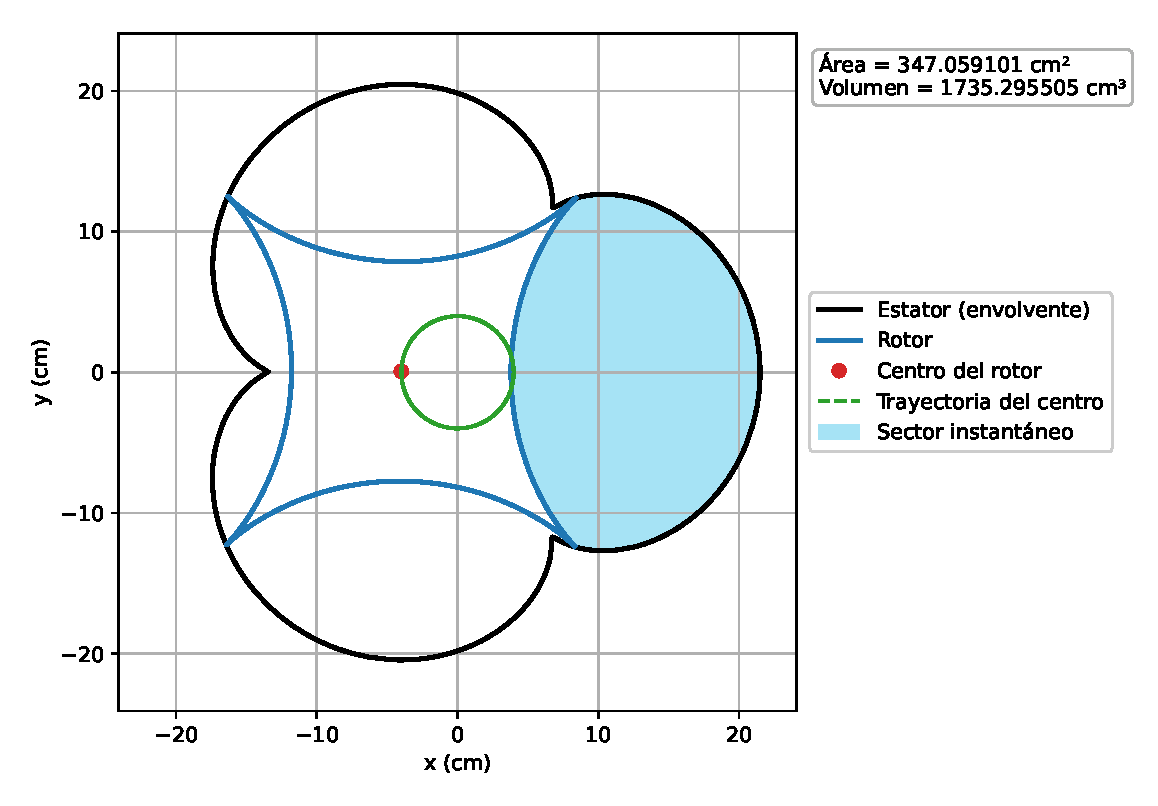
\includegraphics[width=\textwidth]{imagenes/motor_volumen_version_final.eps}
    \caption{Motor Wankel de seis tiempos: arquitectura de tres lóbulos (rotor de cuatro lados).}
    \label{fig:camara-3lob}
  \end{subfigure}
  \hfill
  \begin{subfigure}[t]{0.48\textwidth}
    \centering
    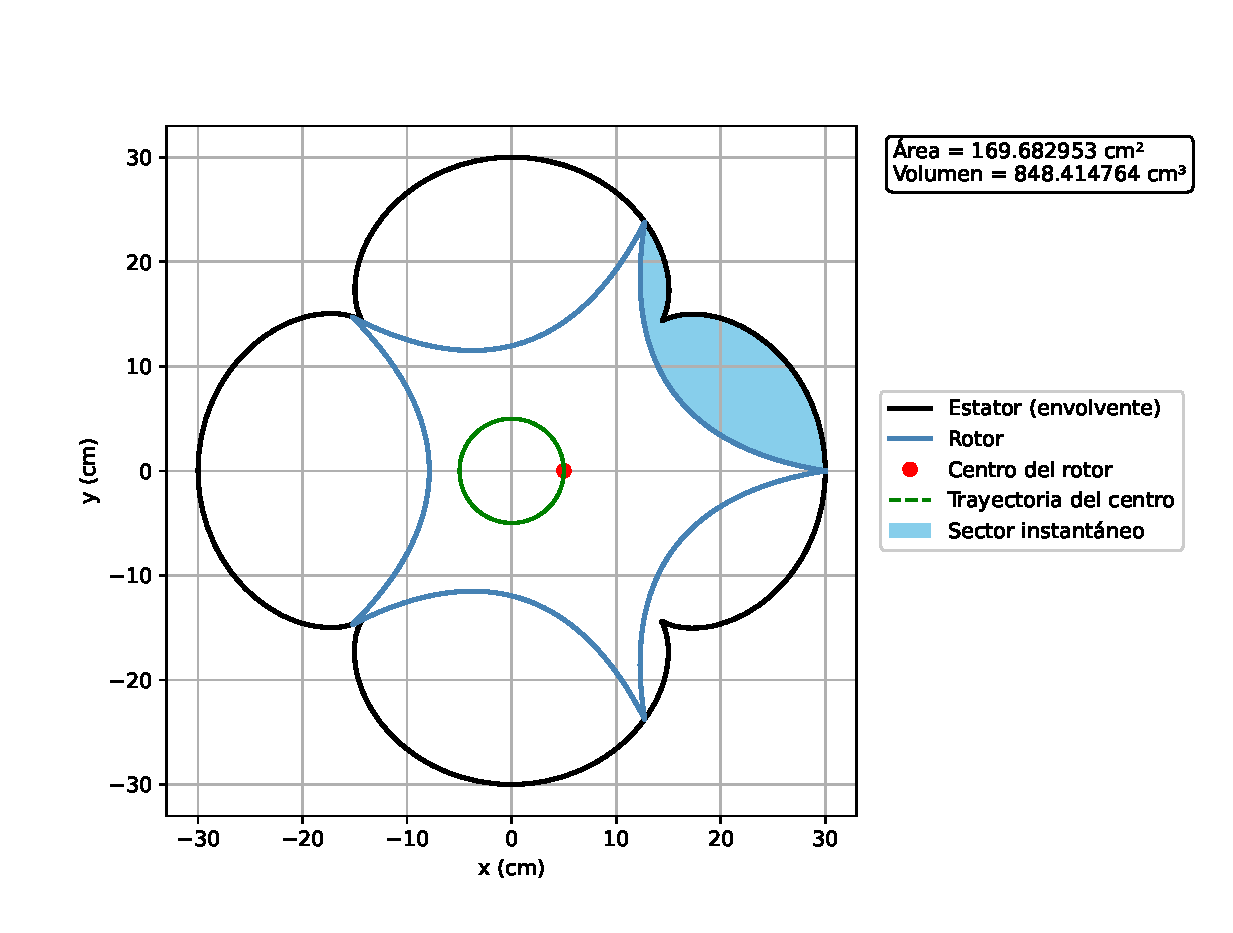
\includegraphics[width=\textwidth]{imagenes/figura_rotor.eps}
    \caption{Motor Wankel de seis tiempos: arquitectura de cuatro lóbulos (rotor de cinco lados).}
    \label{fig:camara-4lob}
  \end{subfigure}
  \caption{Configuraciones geométricas del motor Wankel de seis tiempos.}
  \label{fig:comparacion-lobulos}
\end{figure}



Definidas las posibles arquitecturas, se procede a describir los parámetros geométricos fundamentales que gobiernan la relación cinemática y volumétrica del conjunto rotor–estator, los cuales constituyen la base del modelo computacional desarrollado. A partir de estas configuraciones se plantean tres variantes del motor Wankel de seis tiempos, descritas a continuación:

\textbf{Caso A.} Corresponde a la geometría del motor Wankel de seis tiempos con tres lóbulos y cuatro puntas del rotor (Figura~\ref{fig:camara-3lob}), denominado supercharger. Este nombre se debe a que el motor realiza las fases de compresión y combustión iniciales, y durante la expansión, antes de alcanzar el volumen máximo, se inyecta aire fresco presurizado mediante un sobrealimentador (supercharger). Posteriormente, sin permitir la liberación de los gases de escape, la mezcla de aire fresco y gases calientes comprimidos produce una segunda compresión, seguida de una segunda combustión y una expansión final, tras la cual se evacúan todos los gases.

\textbf{Caso B.} En esta configuración, también basada en la geometría de tres lóbulos y cuatro puntas (Figura~\ref{fig:camara-3lob}), el motor Wankel de seis tiempos opera de forma convencional durante las tres primeras fases: compresión, combustión y expansión. No obstante, al alcanzar el volumen mínimo durante la segunda compresión, se evita la expulsión de los gases de escape y se inyecta agua líquida, la cual se evapora instantáneamente debido a la alta temperatura de los gases residuales. Este cambio de fase genera una segunda expansión impulsada por el vapor de agua, tras la cual ocurre la fase de expulsión de gases.

\textbf{Caso C.} Se emplea una geometría del motor Wankel de seis tiempos con cuatro lóbulos y cinco puntas del rotor (Figura~\ref{fig:camara-4lob}). El proceso inicia con la compresión, combustión y expansión convencionales; sin embargo, en lugar de liberar los gases directamente al ambiente a través de la válvula de escape, estos se conducen hacia una válvula de expansión que reduce su presión hasta condiciones atmosféricas, manteniendo una alta temperatura. A continuación, en la siguiente fase de admisión, se introduce aire fresco junto con los gases calientes de recirculación, dando lugar a una segunda compresión, una segunda combustión y finalmente una expansión complementaria, con lo cual se completa el ciclo de seis tiempos.


A continuación, se describen los parámetros utilizados para la construcción de ambas configuraciones geométricas, tanto la correspondiente al rotor de tres lóbulos (Figura~\ref{fig:camara-3lob}) como la de cuatro lóbulos (Figura~\ref{fig:camara-4lob}), los cuales son comunes para ambas arquitecturas.


\subsection*{Par\'ametros geom\'etricos del motor}

Los par\'ametros \( R \), \( L \) y \( m_{\text{exp}} \) definen la escala, la forma y la cinem\'atica de la geometr\'ia rotor--estator en el motor tipo Wankel.  
Estos tres elementos controlan de manera directa la variaci\'on volum\'etrica de las c\'amaras, la continuidad del sellado y la relaci\'on de compresi\'on del sistema.  
En la Tabla~\ref{tab:param_geom_motor} se resume su interpretaci\'on, importancia funcional y relaci\'on con el dise\~no final del motor.

\begin{table}[H]
\centering
\caption{Resumen de los par\'ametros geom\'etricos principales del motor rotativo tipo Wankel.}
\label{tab:param_geom_motor}
\renewcommand{\arraystretch}{1.35}
\setlength{\tabcolsep}{6pt}
\small
\begin{tabular}{|c|p{4.2cm}|p{4.2cm}|p{4.2cm}|}
\hline
\textbf{Par\'ametro} & \textbf{Interpretaci\'on geom\'etrica} & \textbf{Importancia funcional} & \textbf{Relaci\'on con el dise\~no} \\ 
\hline
\(\boldsymbol{R}\) & 
Distancia entre el centro del rotor y el eje de giro exc\'entrico; determina la trayectoria orbital del rotor. &
Al aumentar \(R\), crece la envolvente y la variaci\'on volum\'etrica, elevando la relaci\'on de compresi\'on. &
En configuraciones 3:4 o 4:5, un incremento moderado de \(R\) mejora el sellado sin interferencias geom\'etricas. \\ 
\hline
\(\boldsymbol{L}\) &
Escala lineal del rotor; representa la distancia desde el centro hasta los \'apices. &
Valores altos de \(L\) pueden causar interferencia; valores bajos reducen el sellado y el volumen \'util. &
El cociente \(L/R\) es cr\'itico para equilibrar compactaci\'on, compresi\'on y suavidad cinem\'atica. \\ 
\hline
\(\boldsymbol{m_{\text{exp}}}\) &
Exponente de la superelipse que controla la redondez del rotor (\(m_{\text{exp}}=2\) circular, \(m_{\text{exp}}=1\) cuadrado). &
Disminuir \(m_{\text{exp}}\) mejora el sellado radial pero incrementa el desgaste; valores mayores suavizan la geometr\'ia. &
Permite optimizar el contacto rotor--estator en dise\~nos de cuatro o cinco caras, evitando picos excesivos de curvatura. \\ 
\hline
\end{tabular}
\end{table}



\subsection*{Relación geométrica entre el estator y el rotor}

La forma interna del estator se obtiene a partir de una curva epitrocoide, generada por la trayectoria de un punto fijo sobre un círculo que rueda externamente sobre otro de mayor radio. Esta curva define el contacto continuo entre los ápices del rotor y el estator, asegurando el sellado durante la rotación.

La epitrocoide se describe mediante:
\[
x(\theta) = (R + r)\cos\theta - d\cos\!\left(\frac{R + r}{r}\theta\right), \qquad
y(\theta) = (R + r)\sin\theta - d\sin\!\left(\frac{R + r}{r}\theta\right),
\]
donde \(R\) es el radio del círculo fijo, \(r\) el del círculo móvil, \(d\) la distancia al punto generador y \(\theta\) el ángulo de rotación. El número de lóbulos del estator depende de la relación entre los radios:
\[
N_e = 1 + \frac{R}{r}.
\]

En el motor Wankel, la correspondencia geométrica se cumple mediante:
\[
N_e = N_r - 1, \qquad \kappa = \frac{1}{N_r},
\]
donde \(N_r\) es el número de caras del rotor, \(N_e\) el número de lóbulos del estator y \(\kappa\) la razón cinemática de giro. Así, un rotor de cuatro caras genera un estator de tres lóbulos (\(\kappa = 1/4\)) y uno de cinco caras, un estator de cuatro lóbulos (\(\kappa = 1/5\)). Esta relación asegura la compatibilidad geométrica y la periodicidad del ciclo rotativo en el modelo del motor.


\subsection{Modelo termodinámico a partir de la gráfica de volumen}

En la sección ecuatorial del motor, el volumen instantáneo de la cámara se obtiene como el producto del espesor axial \(b\) (constante) por el área transversal ocupada por el gas:
\begin{equation}
V(\theta) \;=\; b\,A(\theta).
\label{eq:V=Ab}
\end{equation}

\paragraph{Área como diferencia de radios en coordenadas polares.}
Sea \(\phi\) el ángulo polar tomado desde el centro del estator. Para cada dirección \(\phi\), denótese \(r_{\text{out}}(\phi)\) el radio del contorno del estator, y \(r_{\text{in}}(\phi,\theta)\) el radio del contorno del rotor en la pose \(\theta\). En la configuración \(\theta\), el gas ocupa el anillo radial
\(r\in\big[r_{\text{in}}(\phi,\theta),\,r_{\text{out}}(\phi)\big]\) dentro del sector angular activo \([\phi_1(\theta),\,\phi_2(\theta)]\).
La identidad de área en polares se obtiene integrando el elemento diferencial \(\mathrm{d}A = r\,\mathrm{d}r\,\mathrm{d}\phi\):
\begin{equation}
\begin{aligned}
A(\theta)
&= \int_{\phi_1(\theta)}^{\phi_2(\theta)}
\int_{r_{\text{in}}(\phi,\theta)}^{\,r_{\text{out}}(\phi)}
r\,\mathrm{d}r\,\mathrm{d}\phi
\\[2pt]
&= \frac{1}{2}\int_{\phi_1(\theta)}^{\phi_2(\theta)}
\Big[r_{\text{out}}^2(\phi)-r_{\text{in}}^2(\phi,\theta)\Big]\,\mathrm{d}\phi.
\end{aligned}
\label{eq:area-polares}
\end{equation}
De forma compacta:
\begin{equation}
A(\theta)
= \frac{1}{2}\int_{\phi_1(\theta)}^{\phi_2(\theta)}
\Big[r_{\text{out}}^2(\phi)-r_{\text{in}}^2(\phi,\theta)\Big]\,
\mathrm{d}\phi
\label{eq:area-polar-cont}
\end{equation}


\paragraph{Volumen instantáneo y relación de compresión.}
Sustituyendo \eqref{eq:area-polares} en \eqref{eq:V=Ab} se obtiene el volumen como función del ángulo del rotor:
\begin{equation}
V(\theta) = \frac{b}{2}\int_{\phi_1(\theta)}^{\phi_2(\theta)}
\Big[r_{\text{out}}^2(\phi)-r_{\text{in}}^2(\phi,\theta)\Big]\,
\mathrm{d}\phi
\label{eq:Vtheta-final}
\end{equation}

A partir de \(V(\theta)\) se definen de manera directa los extremos y la relación de compresión del tramo:
\begin{equation}
V_{\max}=\max_{\theta}V(\theta),\qquad
V_{\min}=\min_{\theta}V(\theta),\qquad
r_c=\frac{V_{\max}}{V_{\min}}.
\label{eq:rc}
\end{equation}



Sea $V(\theta)$ la función geométrica de volumen y $\{(\theta_i,V_i)\}$ los nodos relevantes del ciclo. Denótese $V_{\max}$ y $V_{\min}$ los volúmenes extremos del tramo, $n_{\mathrm{comp}}$ y $n_{\mathrm{exp}}$ los exponentes politrópicos de compresión y expansión, y $(P_1,T_1)$ el estado en $V_1=V_{\max}$ (inicio de la Compresión~1). En cada proceso se evaluará punto a punto usando $V(\theta)$.



Las ecuaciones base corresponden a expresiones generales que describen el comportamiento termodinámico del motor y se aplican en los tres casos analizados. No obstante, cada configuración emplea un conjunto de ecuaciones específicas que serán detalladas en secciones posteriores. Para la formulación del modelo termo-mecánico se adoptaron varias idealizaciones con el fin de obtener un esquema matemático coherente y computacionalmente manejable. La compresión y la expansión se trataron como procesos politrópicos en cavidades herméticas, sin fugas ni transferencia de calor apreciable. La combustión se modeló como una adición instantánea de energía bajo un proceso isocórico ideal, sin considerar cinética química, frentes de llama ni pérdidas térmicas. El trabajo se calculó únicamente a partir del área bajo la curva \(P(V)\), por lo que corresponde al trabajo indicado sin incluir efectos mecánicos reales como fricción o bombeo. Finalmente, la reacción estequiométrica del combustible se asumió ideal y constante, sin formación de especies secundarias ni variaciones en el poder calorífico. Estas simplificaciones permiten concentrar el análisis en la geometría y en la secuencia de fases del ciclo, manteniendo un modelo estable y representativo.

 

\paragraph{Ecuaciones base.}
\begin{enumerate}[label=\alph*)]
  \item \textbf{Proceso politrópico} $PV^{n}=\mathrm{cte}$ entre estados $1\to 2$:
  \vspace{-6pt}
  \begin{align}
    P_2 &= P_1\!\left(\frac{V_1}{V_2}\right)^{n}, &
    T_2 &= T_1\!\left(\frac{V_1}{V_2}\right)^{n-1}.
    \label{eq:poly-base}
  \end{align}

\item \textbf{Adición de calor iso–córica} ($V=\mathrm{cte}$):
\vspace{-6pt}
\begin{align}
m_{\text{mez}}\,c_{v,\text{mez}}\,(T_f - T_i)
&=\; \eta_{\mathrm{ch}}\,m_{f,\mathrm{burn}}\,\mathrm{LHV} \;-\; Q_{\mathrm{pérd}}, &
P_f &= P_i\,\frac{T_f}{T_i}, \quad V_f = V_i.
\label{eq:isoV-base}
\end{align}


  \item \textbf{Trabajo indicado} sobre $P(V)$:
  \vspace{-6pt}
  \begin{equation}
    W=\int_{V_\mathrm{ini}}^{V_\mathrm{fin}} P(V)\,\mathrm{d}V, 
    \qquad
    W^{(n)}_{1\to 2}=
    \begin{cases}
      \dfrac{P_2V_2-P_1V_1}{\,1-n\,}, & n\neq 1,\\[6pt]
      P_1V_1\ln\!\left(\dfrac{V_2}{V_1}\right), & n=1.
    \end{cases}
    \label{eq:work-base}
  \end{equation}
\end{enumerate}

\paragraph{Estequiometría de referencia (iso–octano).}
\[
\mathrm{C_8H_{18}} + 12.5\,\mathrm{O_2} \rightarrow 8\,\mathrm{CO_2} + 9\,\mathrm{H_2O}, 
\quad
m_{O_2,\mathrm{st}}\!\approx\!3.5~\mathrm{kg_{O_2}}/\mathrm{kg_{fuel}},
\quad
\mathrm{AFR}_{\mathrm{st}}\!\simeq\!14.7,
\]
\[
Y_{O_2} \simeq 0.232

% CASO A
%===========================================================
\subsubsection{Termodinámica — Caso A: sobrealimentación con \emph{supercharger} (plenum)}

El \textbf{Caso A} introduce aire comprimido desde un plenum durante la primera expansión para completar la oxidación de combustible remanente (mezcla rica tras C1).

\paragraph{Secuencia de procesos.}
\begin{enumerate}[label=\arabic*)]
  \item \textbf{Compresión 1} $(V_{\max}\!\to\!V_{\min})$: politrópico con $n_{\mathrm{comp}}$ usando \eqref{eq:poly-base}.
  \item \textbf{Combustión 1} (C1, $V=V_{\min}$): iso–córica con \eqref{eq:isoV-base} y $Q_V=\eta_{\mathrm{ch}}\,m_{f,\mathrm{burn}}\mathrm{LHV}$ (limitada por $O_2$ disponible en C1).
  \item \textbf{Expansión 1 previa a la inyección} $(V_{\min}\!\to\!V_{\mathrm{inj}}^{-})$: politrópico con $n_{\mathrm{exp}}$ vía \eqref{eq:poly-base}.

  \item \textbf{Inyección desde plenum} ($V=V_{\mathrm{inj}}$): salto iso–córico que impone. 

  En el caso del plenum se simplificó el proceso asumiendo que la inyección ocurre mediante un salto iso–córico ideal, sin modelar el flujo real a través de una válvula ni los efectos dinámicos del conducto. Se trató al plenum como un reservorio de presión constante y se añadió únicamente la masa mínima necesaria según la estequiometría, sin considerar procesos de mezcla, difusión o variaciones térmicas. Las expansiones antes y después de la inyección se modelaron como procesos politrópicos para mantener coherencia con el esquema general del modelo.

  
  \begin{equation}
    P_{\mathrm{pl}}\;\ge\;P(\theta_{\mathrm{inj}}^{-})+\Delta P_{\mathrm{margen}},
    \qquad
    P(\theta_{\mathrm{inj}}^{+})=P_{\mathrm{pl}},\; V(\theta_{\mathrm{inj}}^{+})=V_{\mathrm{inj}}.
    \label{eq:plenum-jump}
  \end{equation}
  La masa mínima para estequiometría respecto a $m_{f,\mathrm{left}}$ es
  \begin{equation}
    m_{\text{air,add}}^{\mathrm{st}}=\frac{m_{O_2,\mathrm{st}}}{Y_{O_2}}\,m_{f,\mathrm{left}}.
    \label{eq:air-stoich-C2-compact}
  \end{equation}
  \item \textbf{Expansión 1 posterior a la inyección} $(V_{\mathrm{inj}}\!\to\!V_{\max})$: politrópico con $n_{\mathrm{exp}}$ usando \eqref{eq:poly-base}.
  \item \textbf{Compresión 2}, \textbf{Combustión 2} (C2, $V=V_{\min}$) y \textbf{Expansión 2}: análogas a 1), 2) y 3) usando \eqref{eq:poly-base}–\eqref{eq:isoV-base}, con $m_{f,\mathrm{burn2}}=m_{f,\mathrm{left}}$ si $m_{\text{air,add}}=m_{\text{air,add}}^{\mathrm{st}}$.
\end{enumerate}

\paragraph{Trabajo y balance neto del bloque sobrealimentado.}
El trabajo del bloque inicial es
\[
W_{\mathrm{comp1}}=\int_{V_{\max}}^{V_{\min}}P_{\mathrm{comp1}}(V)\,\mathrm{d}V,
\quad
W_{\mathrm{exp1}}=\int_{V_{\min}}^{V_{\mathrm{inj}}}\!\!P_{\mathrm{pre}}\,\mathrm{d}V
+\int_{V_{\mathrm{inj}}}^{V_{\max}}\!\!P_{\mathrm{post}}\,\mathrm{d}V,
\]

\[
W_\mathrm{neto}^{(A)}
= W_{\mathrm{exp1}} + W_{\mathrm{comp1}}
\]

La ecuación anterior corresponde únicamente a la primera compresión y a la primera expansión, donde tiene lugar la inyección de aire. Para las etapas de compresión 2 y expansión 2, se emplea la ecuación~\eqref{eq:work-base}, aplicando el signo correspondiente en cada caso.


\\
El \emph{margen} frente al consumo del soplador se evalúa con
\begin{align}
T_{\mathrm{pl}} &= T_\mathrm{amb}\!\left[1+\frac{(PR)^{(\gamma-1)/\gamma}-1}{\eta_c}\right],\quad
\rho_{\mathrm{pl}}=\frac{P_{\mathrm{pl}}}{R\,T_{\mathrm{pl}}}, \label{eq:plenum-state}\\
m_{\mathrm{rev}}&=\rho_{\mathrm{pl}}\,D_{\mathrm{sc}}\,\eta_{\mathrm{vol}},\quad
t_{\mathrm{inj}}=\frac{\theta_{\mathrm{fin}}-\theta_{\mathrm{inj}}}{360^\circ}\,\frac{60}{\mathrm{rpm}_{\mathrm{rotor}}},\\
\dot W_{\mathrm{sc}}&\approx \dot m\,c_p\,(T_{\mathrm{pl}}-T_\mathrm{amb}),\quad
\dot m=\frac{m_{\text{air,add}}}{t_{\mathrm{inj}}},\quad
W_{\mathrm{sc,cyc}}\approx \dot W_{\mathrm{sc}}\,t_{\mathrm{inj}},
\end{align}
\begin{center}
    
$W_{\mathrm{margen}}^{(A)}=W_\mathrm{neto}^{(A)}-W_{\mathrm{sc,cyc}}$.
\end{center}



%===========================================================
% CASO B
%===========================================================
\subsubsection{Termodinámica — Caso B: inyección de agua (expansión secundaria)}

El \textbf{Caso B} inyecta agua durante la primera expansión para producir una re–expansión por vaporización. Las etapas comunes (Compresión~1, C1, Expansión~1 previa) usan \eqref{eq:poly-base}–\eqref{eq:isoV-base} como en el Caso~A. El evento específico es la inyección y vaporización del agua a $V=V_{\mathrm{inj}}$.

En el caso de inyección de agua se asumió que la vaporización ocurre de manera instantánea y completa en el punto de volumen mínimo, sin modelar tiempos de evaporación, mezcla o gradientes térmicos dentro de la cavidad. El proceso se trató a volumen constante y se consideró que el vapor se integra homogéneamente con los gases calientes, usando una constante gaseosa equivalente aire–vapor. Asimismo, no se incluyeron pérdidas de calor hacia las paredes ni efectos transitorios asociados a la inyección. Con estas simplificaciones, la expansión posterior se modeló de forma politrópica, manteniendo coherencia con el marco termodinámico general del modelo.


\paragraph{Balance energético de inyección de agua.}
Para una masa $m_{\text{w}}$:
\begin{align}
Q_1 &= m_{\text{w}}\,c_{p,\text{w}}\,(T_{\mathrm{sat}}-T_{\text{w,inj}}), &
Q_2 &= m_{\text{w}}\,h_{\mathrm{vap}}, &
Q_3 &= m_{\text{w}}\,c_{p,\text{v}}\,(T_4-T_{\mathrm{sat}}),
\end{align}
y el equilibrio con la mezcla gaseosa (a volumen casi constante) se escribe:
\begin{equation}
m_{\text{mez}}\,c_{v,\text{mez}}\,(T_4-T_3) + Q_1 + Q_2 + Q_3 = 0.
\label{eq:water-energy}
\end{equation}
La presión posterior resulta de la masa total de gas y vapor:
\begin{equation}
P_4=\frac{(m_{\text{mez}}+m_{\text{w,vap}})\,R_{\mathrm{eq}}\,T_4}{V_{\mathrm{inj}}},
\label{eq:water-pressure}
\end{equation}
con $R_{\mathrm{eq}}$ constante gaseosa equivalente aire–vapor.

Tras la inyección, la Expansión~1 posterior $(V_{\mathrm{inj}}\!\to\!V_{\max})$ se modela con \eqref{eq:poly-base} usando $n_{\mathrm{exp}}$ y estado $(P_4,T_4)$; luego siguen Compresión~2, Combustión~2 y Expansión~2 análogas al marco común. El beneficio térmico proviene de la energía absorbida por el agua (calentamiento, vaporización y eventual sobrecalentamiento) recuperada como trabajo útil adicional y de la reducción de temperatura pico del ciclo.



\subsubsection{Termodinámica — Caso C: Válvula de expansión}
\label{subsec:thermo-casoC}

\begin{enumerate}[label=\arabic*)]
  \item \textbf{Compresión 1} ($V_{\max}\!\to\!V_{\min}$): politrópica con $n_\mathrm{comp}$ usando \eqref{eq:poly-base}.
  \item \textbf{Combustión 1 (C1)} en $V=V_{\min}$: iso--córica con \eqref{eq:isoV-base}.
  \item \textbf{Expansión 1} ($V_{\min}\!\to\!V_{\max}$): politrópica con $n_\mathrm{exp}$ usando \eqref{eq:poly-base}.
  \item \textbf{Purgado (\emph{blowdown}) por válvula}: descarga desde la cámara al plenum (ver Eqs.~\eqref{eq:mdot-valve}--\eqref{eq:dm-dtheta}).
  \item \textbf{Admisión (succión)}: entrada simultánea de EGR caliente del plenum y aire fresco hasta el BDC; el estado al final de la admisión se fija con \eqref{eq:Tmix-adm}--\eqref{eq:m1-adm}.
  \item \textbf{Compresión 2}, \textbf{Combustión 2 (C2)} en $V_{\min}$ e \textbf{Expansión 2}: análogas a 1), 2) y 3) usando \eqref{eq:poly-base}--\eqref{eq:isoV-base}.
\end{enumerate}

\paragraph{Flujo compresible en la válvula (purgado).} En el modelado del blowdown se asumió que el flujo que sale por la válvula es compresible y unidireccional, aplicando las expresiones estándar para orificios sin considerar efectos viscosos, pérdidas en el conducto ni dinámica detallada de la válvula. Se trató el proceso como muy rápido, por lo que se despreciaron transferencias de calor hacia el bloque y se tomó la mezcla como uniformemente mezclada en cada instante. Asimismo, la evolución de la presión, masa y temperatura se resolvió únicamente a partir del balance de masa y energía simplificado, sin modelar fenómenos transitorios adicionales.

Para una válvula con aguas arriba $P_u,T_u$ (cámara) y aguas abajo $P_d$ (plenum),

defínase $pr \equiv P_d/P_u$ y el umbral crítico $pr_\mathrm{crit}=\left(\tfrac{2}{\gamma+1}\right)^{\gamma/(\gamma-1)}$.
El gasto másico a través de un orificio de área efectiva $A_v$ y coeficiente de descarga $C_d$ es
\begin{equation}
\dot m \;=\;
\begin{cases}
C_d\,A_v\,P_u\;\sqrt{\dfrac{\gamma}{R\,T_u}}\left(\dfrac{2}{\gamma+1}\right)^{\!\tfrac{\gamma+1}{2(\gamma-1)}}, 
& pr \le pr_\mathrm{crit} \quad(\text{ahogado}),\\[10pt]
C_d\,A_v\,P_u\;\sqrt{\dfrac{2\gamma}{R(\gamma-1)T_u}\,\bigl(pr^{2/\gamma}-pr^{(\gamma+1)/\gamma}\bigr)},
& pr>pr_\mathrm{crit}\quad(\text{subsónico}).
\end{cases}
\label{eq:mdot-valve}
\end{equation}
Con velocidad angular $\omega$, el balance de masa en variable angular es
\begin{equation}
\frac{dm_c}{d\theta}\;=\;-\frac{1}{\omega}\,\dot m,
\qquad
\frac{dP_c}{d\theta}\;=\;
\frac{R\,T_c}{V}\frac{dm_c}{d\theta}\;-\;\frac{m_c R T_c}{V^2}\frac{dV}{d\theta},
\label{eq:dm-dtheta}  
\end{equation}
donde $V(\theta)$ y $dV/d\theta$ provienen de la geometría del rotor--estator.



\paragraph{Energía durante el purgado.}
Si se desprecia transferencia térmica al bloque durante el corto blowdown y se toma $c_{v,\mathrm{mix}}$ aproximadamente constante por paso,
\begin{equation}
c_{v,\mathrm{mix}}\!\left(m_c\frac{dT_c}{d\theta}+T_c\frac{dm_c}{d\theta}\right)
\;\simeq\;-\frac{P_c}{\omega}\frac{dV}{d\theta},
\qquad\Rightarrow\qquad
\frac{dT_c}{d\theta}
\simeq
-\frac{P_c}{\omega\,c_{v,\mathrm{mix}}\,m_c}\,\frac{dV}{d\theta}
-\frac{T_c}{m_c}\frac{dm_c}{d\theta}.
\label{eq:dT-dtheta-bd}
\end{equation}
Para cerrar el paso se usa la ecuación de estado
\begin{equation}
P_c(\theta)\;=\;\dfrac{m_c(\theta)\,R_\mathrm{mix}(\theta)\,T_c(\theta)}{V(\theta)}.
\label{eq:EOS-bd}
\end{equation}

\paragraph{Admisión (mezcla aire + EGR).} En la etapa de admisión se asumió que el ingreso de aire fresco y gases remanentes ocurre a presión prácticamente constante y con mezclado inmediato, de modo que la mezcla se considera homogénea desde el inicio. Se aplicaron balances másicos y de entalpía simplificados sin modelar la dinámica real del flujo, la estratificación térmica ni pérdidas por fricción en la entrada. Asimismo, la mezcla aire–EGR se trató como un gas ideal con propiedades promedio, y no se incluyeron efectos transitorios asociados al cierre o apertura geométrica del puerto de admisión.


Sea $m_{f,\mathrm{left}}$ el combustible remanente de C1. La masa mínima de aire fresco requerida para estequiometría es
\begin{equation}
m_{a,\mathrm{req}} \;=\; \mathrm{AFR}_\mathrm{st}\;m_{f,\mathrm{left}}.
\label{eq:air-req}
\end{equation}
Si durante la succión entran $m_a$ de aire a $T_{a}$ y $m_r$ de EGR a $T_{r}$ (ambos a presión de plenum $P_\mathrm{adm}$), la temperatura de mezcla al final de la admisión (BDC) por balance de entalpías es
\begin{equation}
T_1 \;=\; \frac{m_a\,c_{p,a}\,T_a \;+\; m_r\,c_{p,r}\,T_r}{m_a\,c_{p,a}+m_r\,c_{p,r}},
\label{eq:Tmix-adm}
\end{equation}
y la constante de gas de la mezcla (aprox.\ másico) es
\begin{equation}
R_{\mathrm{mix}} \;=\; Y_a R_a + Y_r R_r, 
\qquad Y_a=\frac{m_a}{m_a+m_r},\quad Y_r=\frac{m_r}{m_a+m_r}.
\label{eq:Rmix-adm}
\end{equation}
Suponiendo admisión cuasi--isobárica, el estado al final de la admisión (inicio de Compresión 2) queda
\begin{equation}
P_1 = P_{\mathrm{adm}}, 
\qquad
m_1 = m_a + m_r, 
\qquad
m_1\,R_{\mathrm{mix}}\,T_1 \;=\; P_1\,V_{\mathrm{BDC}}.
\label{eq:m1-adm}
\end{equation}

\paragraph{Procesos restantes del ciclo.}
\begin{itemize}
\item \textbf{Compresión 2} ($V_{\max}\!\to\!V_{\min}$): politrópica con $n_\mathrm{comp2}$ usando \eqref{eq:poly-base}.
\item \textbf{Combustión 2 (C2)} en $V=V_{\min}$: iso--córica con \eqref{eq:isoV-base}, ahora con $m_{f,\mathrm{burn2}}$ y $m_{\mathrm{mez}}=m_1$.
\item \textbf{Expansión 2} ($V_{\min}\!\to\!V_{\max}$): politrópica con $n_\mathrm{exp2}$ usando \eqref{eq:poly-base}.
\end{itemize}

\paragraph{Trabajo indicado por etapas.}
Con $P(V)$ de cada tramo, el trabajo indicado se evalúa con \eqref{eq:work-base}. En particular:
\begin{align}
W_{\mathrm{comp1}} &= \int_{V_{\max}}^{V_{\min}} P_{\mathrm{comp1}}(V)\,dV,
&
W_{\mathrm{exp1}} &= \int_{V_{\min}}^{V_{\max}} P_{\mathrm{exp1}}(V)\,dV,
\\
W_{\mathrm{bd}} &\approx \int_{\theta_{\max}}^{\theta_{\min}} P_c(\theta)\,\frac{dV}{d\theta}\,d\theta\quad(<0),
&
W_{\mathrm{comp2}} &= \int_{V_{\max}}^{V_{\min}} P_{\mathrm{comp2}}(V)\,dV,
\\
W_{\mathrm{exp2}} &= \int_{V_{\min}}^{V_{\max}} P_{\mathrm{exp2}}(V)\,dV.
\end{align}
El balance del ciclo del Caso C (sin pérdidas mecánicas) es
\begin{equation}
W^{(C)}_{\mathrm{neto}} 
\;=\; 
W_{\mathrm{exp1}} + W_{\mathrm{exp2}}
\;-\;
\bigl|W_{\mathrm{comp1}}\bigr| - \bigl|W_{\mathrm{comp2}}\bigr|
\;+\; W_{\mathrm{bd}}.
\end{equation}

\paragraph{Condición admisión de aire.}
Si se persigue estequiometría estricta para C2, se impone
\begin{equation}
m_a(\theta)\uparrow\; \text{hasta}\; m_{a,\mathrm{req}}\quad\Rightarrow\quad \dot m_a\!\to\!0\;\text{(cierre de válvula de aire)},
\end{equation}


\subsubsection{Torque }

Se definió el vector $\vec{r}$ desde el origen hasta la mitad geométrica del lado, punto donde actúa la presión promedio del gas. La fuerza se calculó como
\begin{equation}
\vec{F} = P\,A\,\hat{n},
\end{equation}
donde $P$ es la presión interna instantánea, $A$ el área efectiva de la cara del rotor y $\hat{n}$ el vector normal negativo a la superficie. Con ambos vectores se obtuvo el torque instantáneo mediante
\begin{equation}
\vec{\tau} = \vec{r} \times \vec{F},
\end{equation}

\paragraph{Cálculo de la potencia.}
A partir del torque promedio obtenido, se determinó la potencia nominal se expresa como:

\begin{equation}
P = \tau\,\omega,
\label{ptw}
\end{equation}


\subsubsection{Eficiencia térmica}


\begin{equation}
W_{\text{neto}} = \oint P\, dV
\label{eq:Trabajo_Neto}
\end{equation}

El calor total aportado al ciclo corresponde a la suma de las liberaciones de energía de las dos combustiones iso-córicas modeladas:

\begin{equation}
Q_{\text{in}} = Q_{\text{rel,C1}} + Q_{\text{rel,C2}}
\end{equation}

\begin{equation}
\eta_t = \frac{W_{\text{neto}}}{Q_{\text{in}}}
\end{equation}


\subsubsection{Implementación Discreta}

En esta sección se presenta la discretización de las ecuaciones analíticas para su implementación numérica mediante herramientas computacionales. Este proceso permite modelar el comportamiento del motor y obtener los resultados necesarios para comparar los distintos casos analizados.

\textbf{Área y volumen:} Se implementaron las expresiones geométricas del capítulo anterior: el área transversal \(A(\theta)\) según \eqref{eq:area-polares}, el volumen instantáneo \(V(\theta)=b\,A(\theta)\) de \eqref{eq:Vtheta-final}, y los extremos \(V_{\max},V_{\min}\) con la relación de compresión \(r_c\) definidos en \eqref{eq:rc}. Con estas ecuaciones se generaron las rutinas numéricas y las curvas \(V(\theta)\) que alimentan el modelo termodinámico.


\paragraph{Implementación discreta con sumatorias.}
Se discretiza el ciclo con \(N_\theta\) poses y el sector angular con \(N_{\text{int}}\) puntos:
\[
\theta_i=\frac{2\pi i}{N_\theta},\quad i=0,\dots,N_\theta-1,
\qquad
\phi^{(i)}_\ell=\phi_1(\theta_i)+\ell\,\frac{\Delta\phi^{(i)}}{N_{\text{int}}-1},\ 
\Delta\phi^{(i)}=\big(\phi_2(\theta_i)-\phi_1(\theta_i)\big)\bmod 2\pi,
\ \ell=0,\dots,N_{\text{int}}-1.
\]
Para cada par \((i,\ell)\) se evalúan:
\begin{itemize}
  \item \(r_{\text{out}}(\phi^{(i)}_\ell)\) por interpolación periódica de una tabla radial del estator.
  \item \(r_{\text{in}}(\phi^{(i)}_\ell,\theta_i)\) como el \emph{primer} cruce del rayo \(\mathbf{r}(s)=s(\cos\phi^{(i)}_\ell,\sin\phi^{(i)}_\ell)\) con el polígono del rotor en la pose \(\theta_i\). Para cada arista \(j=0,\dots,N_e-1\), con extremos \(\mathbf{P}^{(i)}_j,\mathbf{P}^{(i)}_{j+1}\), se resuelve \(\mathbf{r}(s)=\mathbf{P}^{(i)}_j+t(\mathbf{P}^{(i)}_{j+1}-\mathbf{P}^{(i)}_j)\). Se aceptan soluciones con \(t\in[0,1]\), \(s\ge 0\); se toma \(r_{\text{in}}=\min s\). Si no hay cruce, se impone \(r_{\text{in}}=r_{\text{out}}\).
\end{itemize}

Con estas muestras, la integral \eqref{eq:area-polar-cont} se aproxima por trapecios en \(\phi\). Sea
\[
g^{(i)}_\ell \;=\; \big[r_{\text{out}}(\phi^{(i)}_\ell)\big]^2-\big[r_{\text{in}}(\phi^{(i)}_\ell,\theta_i)\big]^2,
\qquad
\Delta\phi^{(i)}_\ell=\phi^{(i)}_{\ell+1}-\phi^{(i)}_\ell.
\]
Entonces, el área y el volumen en la pose \(i\) son
\begin{equation}
A_i \;\approx\; \frac{1}{2}\sum_{\ell=0}^{N_{\text{int}}-2}
\frac{\Delta\phi^{(i)}_\ell}{2}\,\Big(g^{(i)}_\ell+g^{(i)}_{\ell+1}\Big),
\qquad
V_i \;=\; b\,A_i,
\label{eq:area-trapecios}
\end{equation}
y los extremos discretos se obtienen con
\[
V_{\max}=\max_{0\le i<N_\theta} V_i,\qquad
V_{\min}=\min_{0\le i<N_\theta} V_i,\qquad
r_c=\frac{V_{\max}}{V_{\min}}.
\]

\paragraph{Esquema iterativo (índices).}
\begin{align*}
&\textbf{Para } i=0,\dots,N_\theta-1: \\
&\quad \text{(1) Construir } \{\phi^{(i)}_\ell\}_{\ell=0}^{N_{\text{int}}-1} \text{ desde } \phi_1(\theta_i)\to\phi_2(\theta_i).\\
&\quad \text{(2) Para } \ell=0,\dots,N_{\text{int}}-1:
\ \ r_{\text{out}}(\phi^{(i)}_\ell),\ \ r_{\text{in}}(\phi^{(i)}_\ell,\theta_i) \ \Rightarrow\ g^{(i)}_\ell.\\
&\quad \text{(3) } A_i \text{ y } V_i \text{ con \eqref{eq:area-trapecios}.}
\end{align*}

\textbf{Termodinámica:} Partiendo de los vectores discretos $\{(\theta_i,V_i)\}_{i=0}^{N_\theta-1}$ del capítulo geométrico, los procesos termodinámicos se resuelven punto a punto usando las ecuaciones base ya establecidas: la ley politrópica (\ref{eq:poly-base}), la adición de calor iso–córica (\ref{eq:isoV-base}) y el trabajo indicado (\ref{eq:work-base}). A continuación se detalla la implementación \emph{general} de los tres procesos básicos y, después, las particularidades:

\begin{enumerate}[label=\arabic*)]
  \item \textbf{Compresión politrópica} sobre un tramo $V_i\!\downarrow$: se avanza con (\ref{eq:poly-base})
  \[
    P_{i+1} = P_i\!\left(\frac{V_i}{V_{i+1}}\right)^{n_{\mathrm{comp}}},\qquad
    T_{i+1} = T_i\!\left(\frac{V_i}{V_{i+1}}\right)^{n_{\mathrm{comp}}-1}.
  \]
  \item \textbf{Combustión iso–córica} en $V=\text{cte}$ (nodo $j$): se aplica (\ref{eq:isoV-base}) para actualizar $T_{j+1}$ y $P_{j+1}=P_j(T_{j+1}/T_j)$.
  \item \textbf{Expansión politrópica} sobre un tramo $V_i\!\uparrow$: se avanza con (\ref{eq:poly-base})
  \[
    P_{i+1} = P_i\!\left(\frac{V_i}{V_{i+1}}\right)^{n_{\mathrm{exp}}},\qquad
    T_{i+1} = T_i\!\left(\frac{V_i}{V_{i+1}}\right)^{n_{\mathrm{exp}}-1}.
  \]
\end{enumerate}

\textbf{Torque:} El cálculo del torque se implementó a partir de la formulación vectorial descrita anteriormente, discretizada para su resolución numérica. Se definió el vector de posición $\vec{r}_i$ desde el origen hasta el punto medio del lado del rotor en la pose angular $\theta_i$, y el vector normal negativo $\hat{n}_i$ asociado a dicha cara. La fuerza instantánea se calculó como
\[
\vec{F}_i = P_i\,A\,\hat{n}_i,
\]
donde $P_i$ es la presión interna para el ángulo $\theta_i$ y $A$ el área de la cara del rotor.  

El torque discreto se obtuvo mediante
\[
\vec{\tau}_i = \vec{r}_i \times \vec{F}_i,
\]
cuyo módulo $\tau_i = \|\vec{\tau}_i\|$ representa el par generado en cada posición angular.  

El ciclo se discretizó en $N_\theta$ posiciones equiespaciadas, sumando los torques de cada cámara con el desfase angular correspondiente ($90^\circ$ para cuatro cámaras y $72^\circ$ para cinco). La integración de estas contribuciones permitió construir la curva de torque total.  

Finalmente, se verificó la conservación de momentos, garantizando que el signo del torque reflejara el sentido físico de rotación: positivo en expansión y negativo en compresión.


\subsection{Simulación Computacional}


Con el fin de integrar las relaciones geométricas del motor Wankel con un modelo termo–mecánico capaz de representar un ciclo extendido de seis tiempos, se desarrolló una herramienta computacional modular en Python. Esta herramienta constituye el eje central del proyecto, pues permite vincular la geometría del estator y del rotor con los procesos termodinámicos del ciclo, generando resultados comparables entre diferentes configuraciones. Su estructura se diseñó para que la modificación de parámetros geométricos y operativos no requiera alterar la lógica fundamental del modelo, lo que facilita la exploración de nuevas variantes y la validación del comportamiento del motor bajo distintos escenarios.

El modelo recibe como entrada las relaciones geométricas que definen la arquitectura del motor, incluyendo el número de lóbulos del estator, el número de puntas del rotor, la excentricidad y las dimensiones fundamentales del  presentadas mas adelante. También incorpora las condiciones iniciales de operación, tales como la presión y la temperatura en la admisión, los exponentes politrópicos para los procesos de compresión y expansión, la masa admitida de la mezcla y el valor energético del combustible. Adicionalmente, el usuario puede seleccionar la configuración del ciclo que desea simular, ya sea la variante con sobrealimentación, con inyección de agua o con válvula de expansión.

A partir de estas entradas, la herramienta genera como salida las funciones de volumen instantáneo en función del ángulo del rotor, las curvas de presión y temperatura para cada fase del ciclo, los diagramas presión–volumen (P–V) asociados a los procesos politrópicos y isocóricos, y el trabajo indicado obtenido mediante la integración numérica de dichas curvas. El modelo también calcula el torque instantáneo y el torque promedio aplicando formulaciones vectoriales, y a partir de estos valores estima la potencia indicada del motor en función del régimen de giro. Finalmente, la herramienta produce un conjunto de resultados comparativos que permiten evaluar el desempeño de cada configuración frente al motor Wankel convencional de cuatro tiempos.

El funcionamiento de la herramienta se organiza en cuatro etapas consecutivas. En primer lugar, el módulo geométrico determina el volumen instantáneo de cada cavidad empleando la curva epitrocoidal del estator y la cinemática del rotor. Posteriormente, el módulo termo–mecánico resuelve los procesos politrópicos de compresión y expansión, así como los procesos isocóricos correspondientes a las combustiones del ciclo. Luego, el módulo energético integra los diagramas P–V para obtener el trabajo indicado y calcula el calor suministrado en cada una de las combustiones. Finalmente, el módulo dinámico determina las fuerzas sobre las caras del rotor, calcula el torque y construye las curvas de potencia en función de la velocidad angular. Esta arquitectura modular permite simular nuevas geometrías y extender el modelo a configuraciones alternativas sin modificar su estructura esencial, consolidando un marco de simulación adaptable para el análisis termo–mecánico de motores Wankel de múltiples tiempos.


Las curvas presentadas a continuación se obtuvieron a partir de las muestras discretas 
\(\{(\theta_i, V_i)\}_{i=0}^{N_\theta-1}\), calculadas mediante la ecuación 
\eqref{eq:area-trapecios}. A partir de esta construcción se generan todas las gráficas 
\(V\)–\(\theta\) mostradas en el documento: en primer lugar, se calcula \(V_i\) empleando 
la ecuación \eqref{eq:area-trapecios}; posteriormente, los valores de \(\theta_i\) se 
convierten a grados; y finalmente, se representan los pares ordenados 
\((\theta_i, V_i)\). 

Como se mencionó anteriormente, se desarrollaron dos configuraciones geométricas: una 
correspondiente a un rotor de tres lóbulos y otra de cuatro lóbulos. A continuación, se 
presentan las gráficas de volumen en función del ángulo para cada una de estas 
geometrías.

\begin{figure}[H]
  \centering

  % --- Subfigura 1 ---
  \begin{subfigure}[b]{0.48\textwidth}
    \centering
    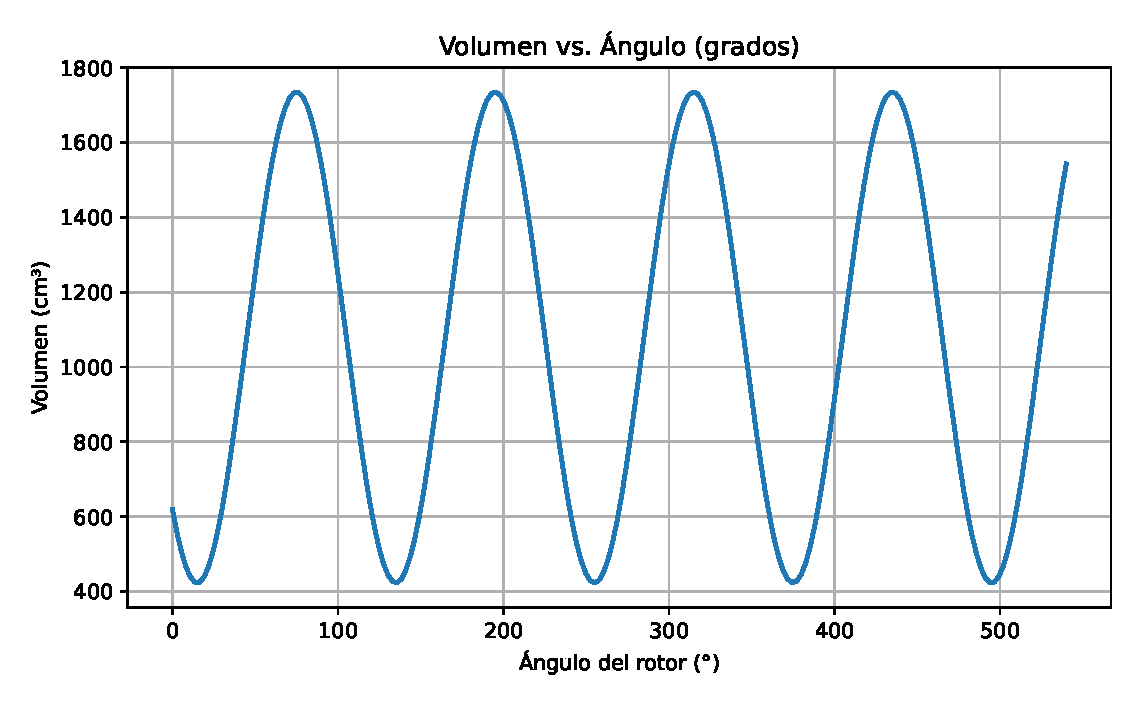
\includegraphics[width=\textwidth]{imagenes/volumen_vs_angulo_deg_VERSION.eps}
    \caption{Arquitectura de tres lóbulos (rotor de cuatro lados).}
    \label{fig:vol_3lob}
  \end{subfigure}
  \hfill
  % --- Subfigura 2 ---
  \begin{subfigure}[b]{0.5\textwidth}
    \centering
    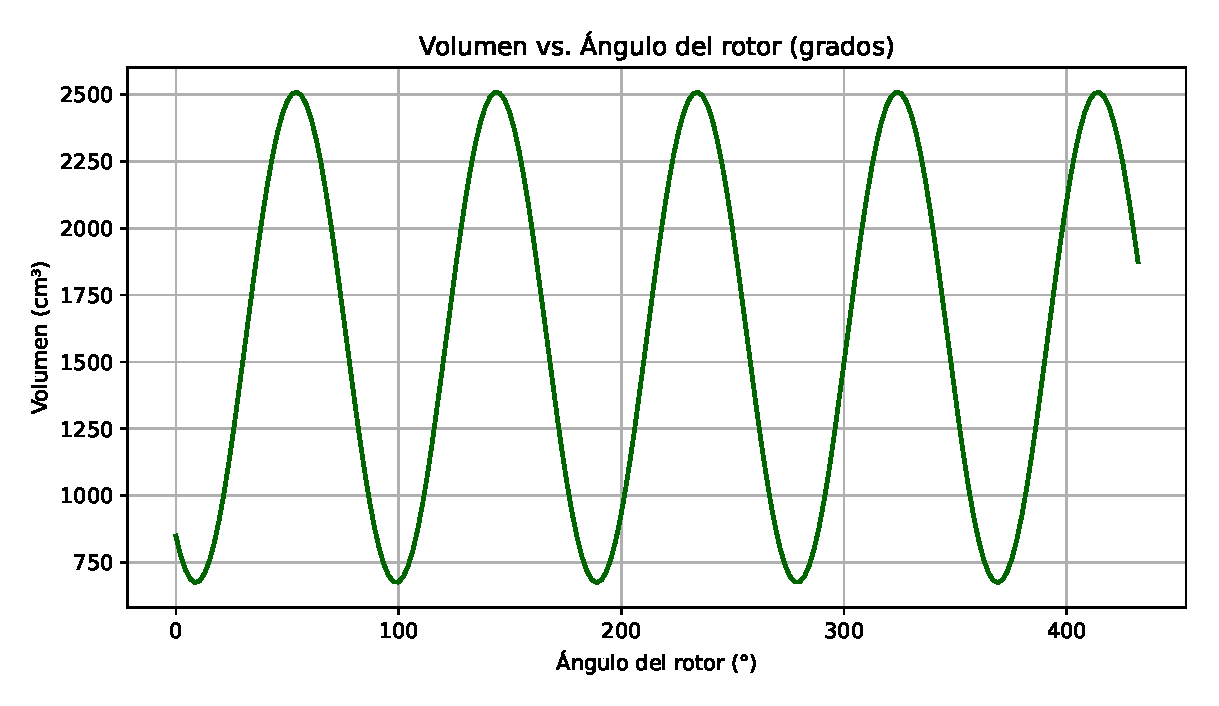
\includegraphics[width=\textwidth]{imagenes/volumen_vs_angulo_grados_4lobulos_versionfinal.eps}
    \caption{Arquitectura de cuatro lóbulos (rotor de cinco lados).}
    \label{fig:vol_4lob}
  \end{subfigure}

  \caption{Comparación del volumen instantáneo para una cavidad individual en motores Wankel de seis tiempos: (a) tres lóbulos y (b) cuatro lóbulos.}
  \label{fig:comparacion_3vs4lob}
\end{figure}

La comparación entre ambas gráficas evidencia que aumentar el número de lóbulos modifica tanto la frecuencia como la amplitud de las variaciones volumétricas por revolución. En la configuración de tres lóbulos se presentan cuatro ciclos por giro, con volúmenes entre 423~cm\textsuperscript{3} y 1735~cm\textsuperscript{3}. En la de cuatro lóbulos, el estator genera cinco ciclos, reduciendo el periodo angular en aproximadamente 18° y ampliando el rango volumétrico a 673--2509~cm\textsuperscript{3}, lo que se traduce en un mayor desplazamiento efectivo. La arquitectura de cuatro lóbulos también distribuye mejor las fases simultáneas, aportando mayor simetría dinámica, mientras que la de tres lóbulos tiende a presentar mayor asimetría térmica por la ubicación de las bujías.

\begin{figure}[H]
  \centering

  % --- Subfigura 1: 4 fases (3 lóbulos) ---
  \begin{subfigure}[b]{0.51\textwidth}
    \centering
    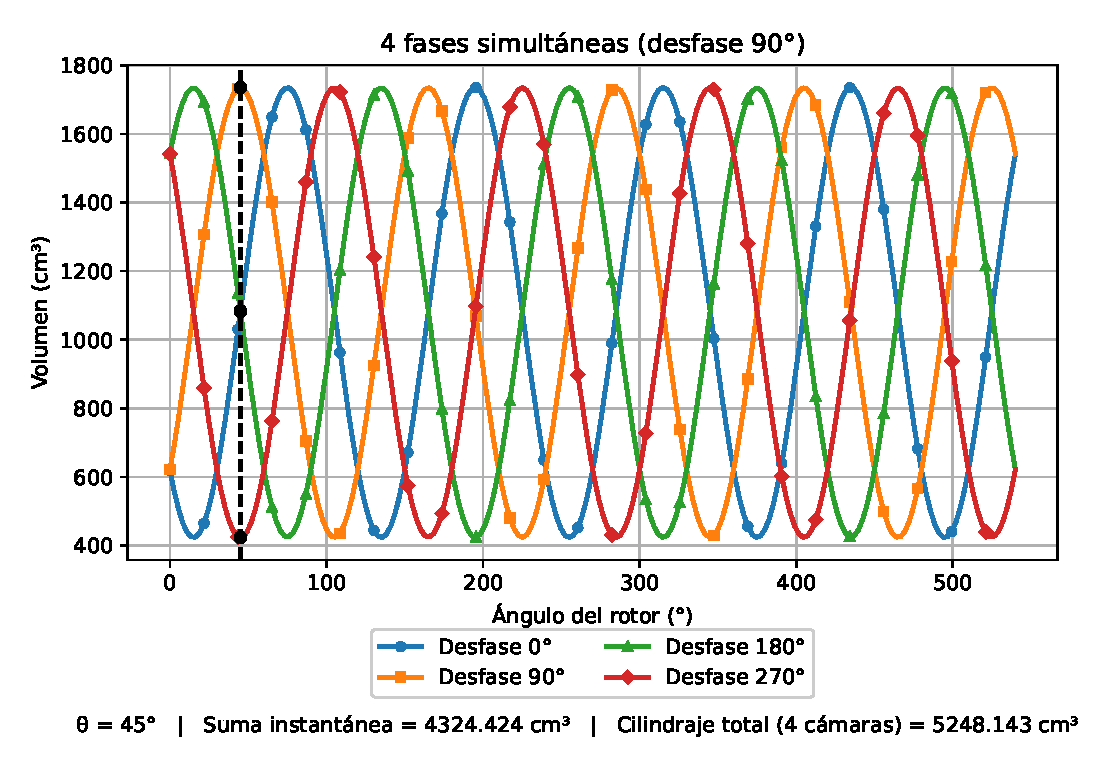
\includegraphics[width=\textwidth]{imagenes/volumen_vs_angulo_4fases_90deg_versionfinal.eps}
    \caption{Arquitectura de tres lóbulos (rotor de cuatro lados).}
    \label{fig:4fases_3lob}
  \end{subfigure}
  \hfill
  % --- Subfigura 2: 5 fases (4 lóbulos) ---
  \begin{subfigure}[b]{0.46\textwidth}
    \centering
    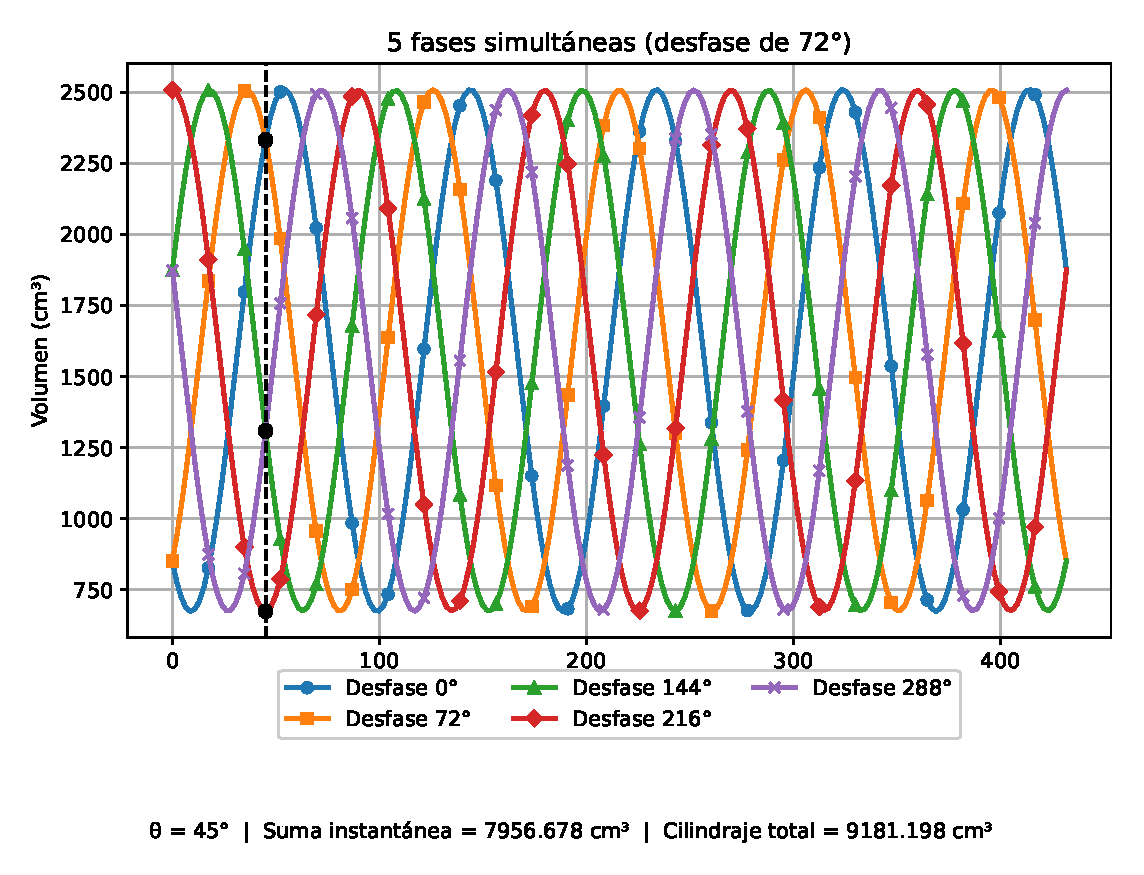
\includegraphics[width=\textwidth]{imagenes/volumen_5fases_lineas_continuas_marcadores_medianos_2.eps}
    \caption{Arquitectura de cuatro lóbulos (rotor de cinco lados).}
    \label{fig:5fases_4lob}
  \end{subfigure}

  \caption{Comparación del comportamiento volumétrico instantáneo: (a) cuatro cavidades desfasadas 90° en la arquitectura de tres lóbulos y (b) cinco cavidades desfasadas 72° en la arquitectura de cuatro lóbulos.}
  \label{fig:comparacion_fases_3vs4lob}
\end{figure}

Las gráficas muestran cómo el aumento en el número de lóbulos incrementa la cantidad de cavidades operando simultáneamente y reduce el periodo angular entre ciclos. En la configuración de tres lóbulos, cuatro cavidades actúan con un desfase de 90°, mientras que en la de cuatro lóbulos intervienen cinco cavidades con un desfase de 72°, generando una mayor continuidad volumétrica y un cilindraje instantáneo superior en cada giro. A continuación se presentarán los 3 casos de estudio planteados para las 2 geometrías mencionadas previamente 


\subsubsection{Termodinámica —(Caso A Supercharger)}

En esta sección se mostrarán los resultados relevantes del estudio de un motor con un ciclo térmico modificado de 6 tiempos con un compresor 

\begin{figure}[H]
    \centering
    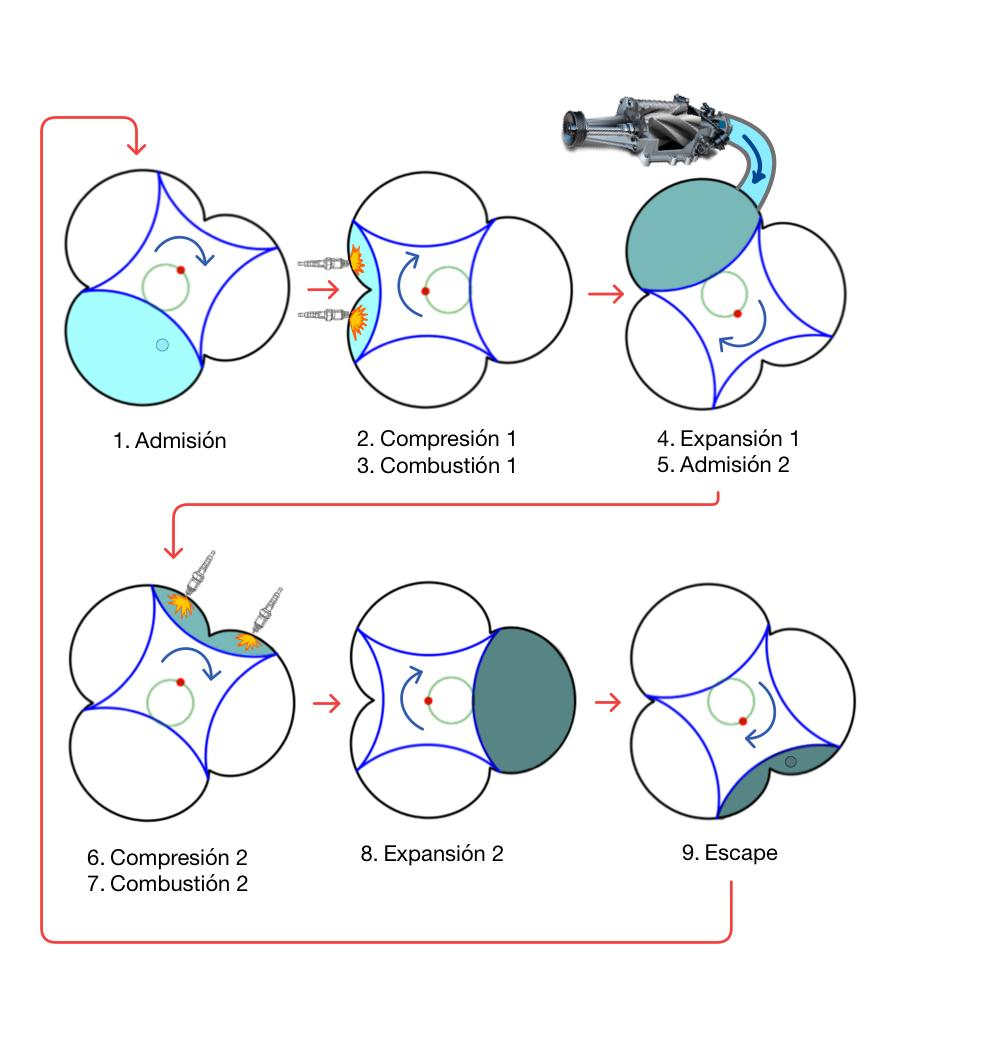
\includegraphics[width=0.55\textwidth]{superch.jpg}
    \caption{Diagrama de funcionamiento del \textbf{Caso A} (sobrealimentación con \emph{supercharger}) para el motor Wankel de seis tiempos. Fuente: elaboración propia}
    \label{fig:motor_casoA}
\end{figure}

La figura presenta la secuencia de un ciclo modificado de nueve etapas para un motor Wankel de seis tiempos. El proceso inicia con la admisión, donde la cavidad capta la mezcla fresca. Luego se desarrolla la primera compresión, seguida de la primera combustión, que genera la primera expansión. Durante esta expansión tiene lugar una segunda admisión que introduce aire adicional para la siguiente etapa. A continuación, la cavidad entra en la segunda compresión, culminando en una segunda combustión que origina la segunda expansión del ciclo. Finalmente, los productos de la reacción se evacuan en la fase de escape, completando así el conjunto de seis tiempos que combina dos procesos de combustión en un mismo giro del rotor.

\begin{figure}[H]
    \centering
    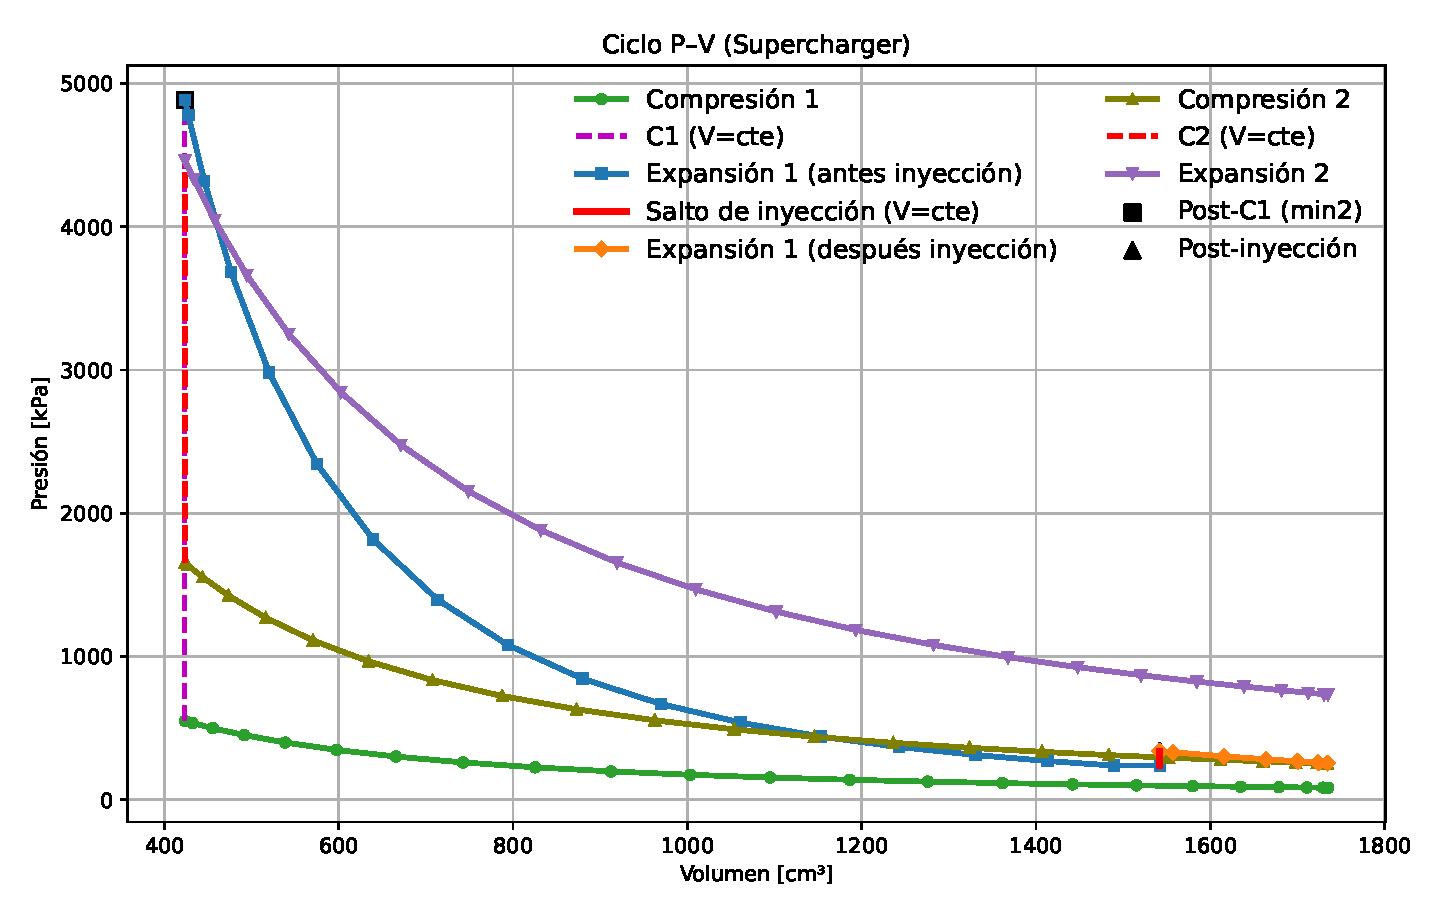
\includegraphics[width=0.6\textwidth]{imagenes/ciclo_PV_supercharger_color_versionfinal2.eps}
    \caption{Diagrama $P$–$V$ del \textbf{Caso A} (sobrealimentación con \emph{supercharger}) para el motor Wankel de seis tiempos. Fuente: elaboración propia}
    \label{fig:motor_casoA}
\end{figure}


En este caso, los primeros tiempos de \textit{compresión} y \textit{combustión 1} se desarrollan de manera análoga a los de un motor convencional, siguiendo la ecuación politrópica de referencia \eqref{eq:poly-base} y el proceso isocórico descrito en \eqref{eq:isoV-base}. Posteriormente, antes de la inyección de aire, se lleva a cabo una expansión politrópica estándar, también regida por \eqref{eq:poly-base}.  

En un ángulo determinado del ciclo, se produce la \textit{inyección de aire fresco presurizado} proveniente de un supercargador, el cual introduce el aire a una presión aproximada de \(229~\text{kPa}\). En ese instante, los gases contenidos en la cámara se encontraban alrededor de \(219~\text{kPa}\), motivo por el cual se observa un \textit{pequeño salto de presión} en la gráfica \(P\!-\!V\).  

A continuación, se desarrolla una nueva \textit{compresión politrópica}, seguida de una \textit{segunda combustión}, la cual, al disponer de una cantidad significativamente menor de combustible, \textit{no alcanza presiones máximas tan elevadas} como la primera. Finalmente, el proceso culmina con una expansión politrópica normal que completa el ciclo.

El análisis energético del ciclo permitió determinar que la suma de los calores liberados en las dos combustiones fue de \(Q_{\text{in}} = 8.96~\text{kJ}\), mientras que el trabajo neto obtenido de la integración del diagrama \(P\!-\!V\) correspondió a \(W_{\text{net}} = 4.56~\text{kJ}\). De esta manera, la eficiencia térmica global del motor con supercargador se estimó en aproximadamente \(\eta = 50.91\%\), lo que evidencia una mejora significativa en el aprovechamiento energético del ciclo en comparación con configuraciones convencionales sin sobrealimentación.




\begin{figure}[H]
    \centering    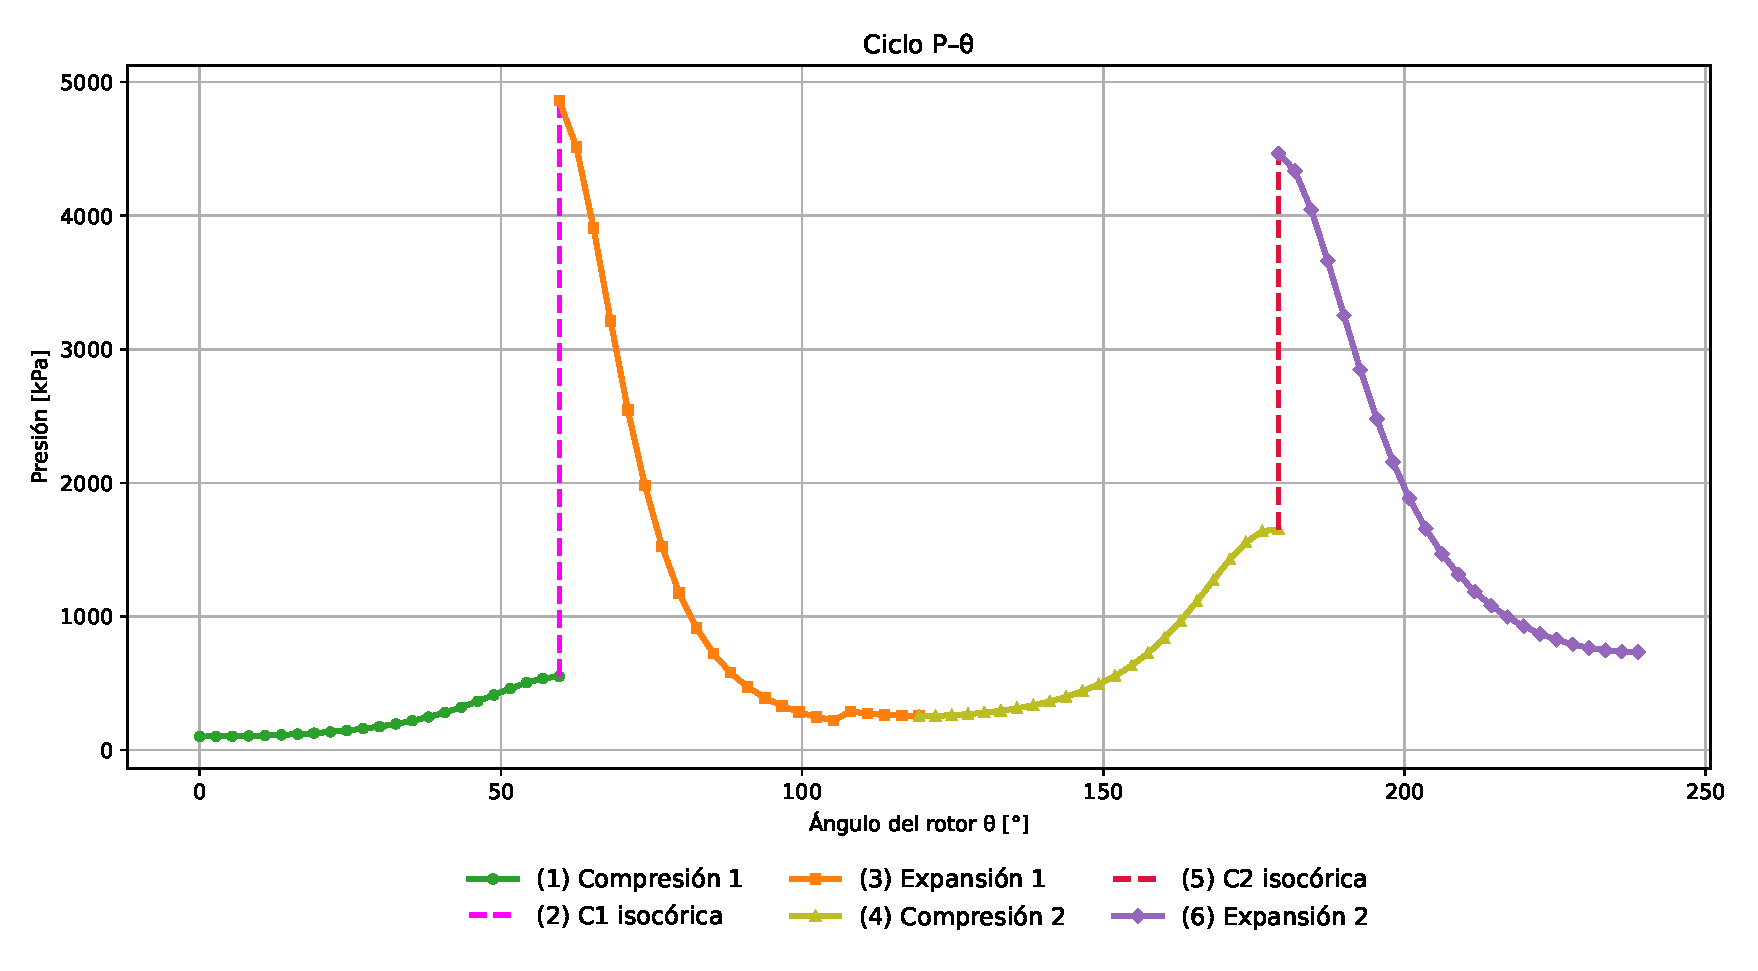
\includegraphics[width=0.7\textwidth]{imagenes/P_vs_theta_ciclo_completo_versionfinal3.eps}
    \caption{Presión con relación al ángulo del rotor del \textbf{Caso A} (sobrealimentación con \emph{supercharger}) para el motor Wankel de seis tiempos. Fuente: elaboración propia}
    \label{fig:presion_angulo}
\end{figure}

La Figura~\ref{fig:presion_angulo} presenta la variación de la presión con respecto al ángulo de rotación del rotor, donde se distinguen claramente las fases de compresión, combustión, expansión con inyección de aire, post compresion , post combustion, y post expansion. Esta gráfica permite identificar el comportamiento instantáneo de la presión en cada punto del ciclo y fue utilizada como base para el análisis termodinámico del motor.

Durante la etapa de expansión se observa una disminución progresiva de la presión dentro de la cámara. Sin embargo, justo antes de alcanzar el volumen máximo, se aprecia un leve incremento en la presión debido a la inyección de aire fresco, ligeramente más frío. Este fenómeno genera un aumento de presión hasta aproximadamente \(229~\text{kPa}\), en comparación con los \(219~\text{kPa}\) presentes en la cámara antes de la inyección. 

A partir de este punto, el proceso de compresión se inicia desde dicho valor de presión inicial, lo que explica que la segunda curva de compresión presente valores superiores a los de la primera, la cual parte desde condiciones de presión atmosférica. Finalmente, tiene lugar la combustión del combustible remanente, seguida de una expansión final que completa el ciclo y restablece las condiciones iniciales de operación.


\begin{figure}[H]
    \centering
    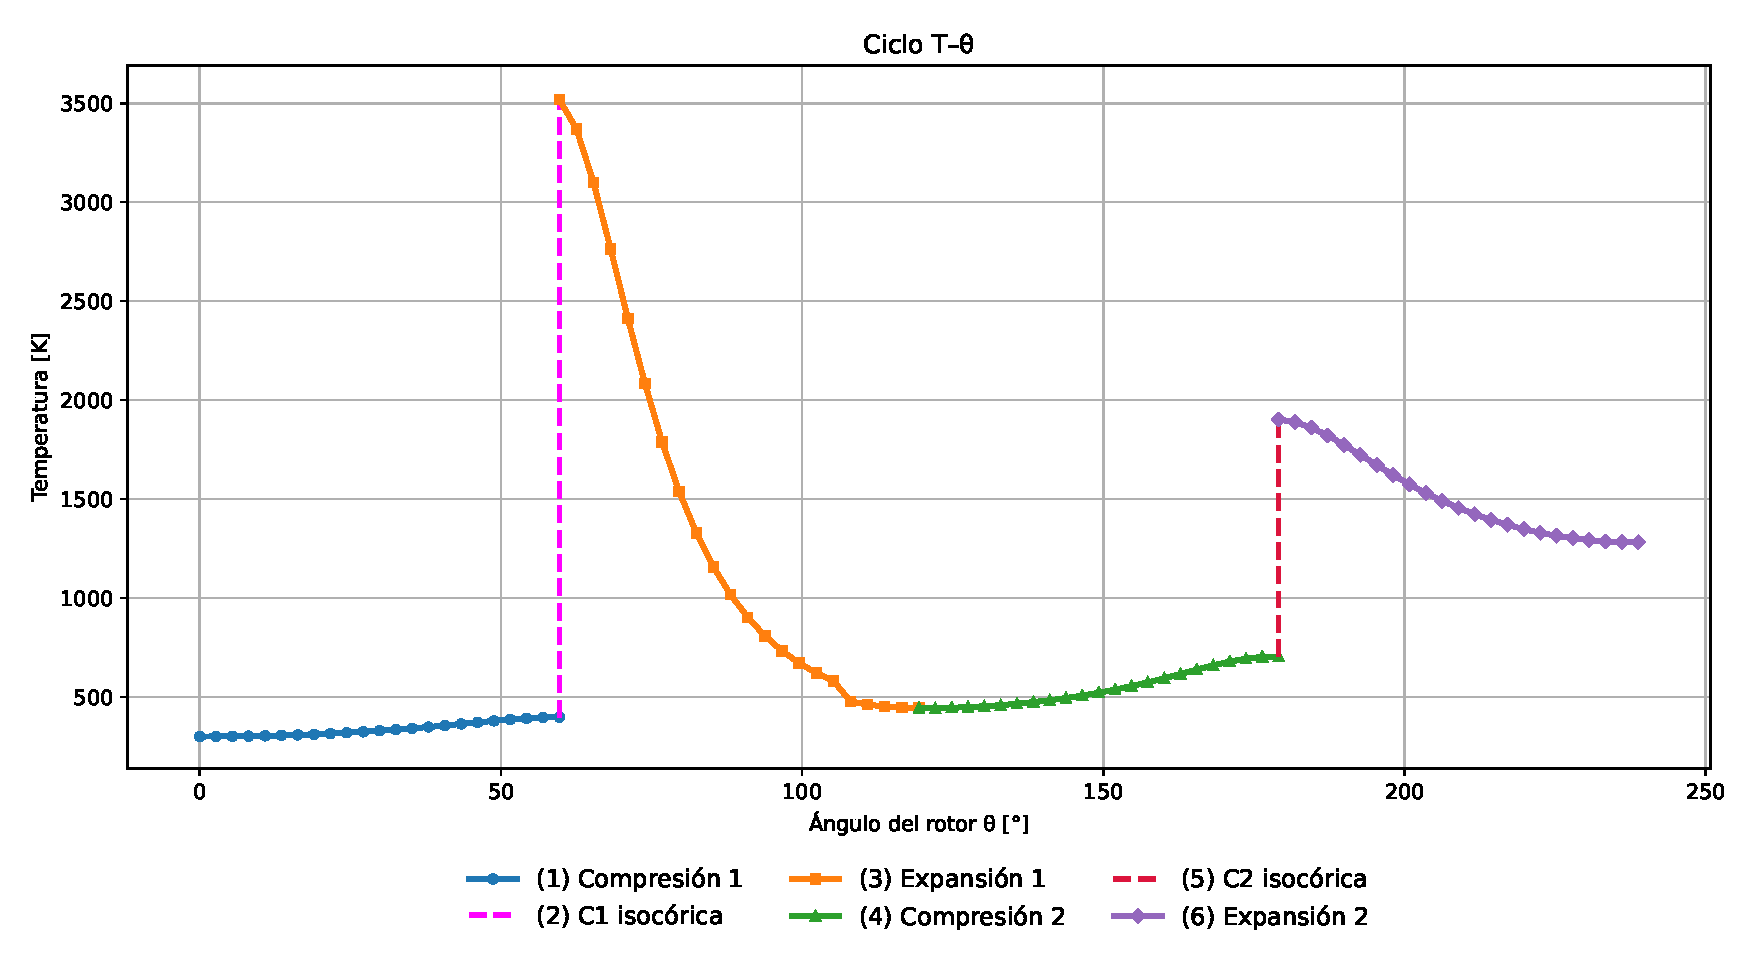
\includegraphics[width=0.7\textwidth]{imagenes/T_theta_ciclo_completo_versionfinal3.eps}
    \caption{Temperatura con relación al ángulo del rotor del \textbf{Caso A} (sobrealimentación con \emph{supercharger}) para el motor Wankel de seis tiempos. Fuente: elaboración propia}
    \label{fig:motor_casoA}
\end{figure}

En esta gráfica se observa la evolución de la temperatura en función del ángulo del rotor a lo largo de las fases del ciclo. Durante la primera compresión y expansión, el comportamiento es similar al de un ciclo convencional, alcanzándose un incremento térmico pronunciado tras la combustión principal. Sin embargo, tras la primera expansión, la presencia del plenum introduce aire fresco frío en la cámara, generando una ligera disminución de la temperatura, lo que contribuye a estabilizar el proceso térmico. Posteriormente, durante la segunda compresión, el aire remanente se mezcla con una cantidad reducida de combustible, produciendo una segunda combustión de menor intensidad. Este fenómeno se traduce en un pico térmico más bajo, coherente con la menor disponibilidad de energía química, pero suficiente para prolongar la expansión y mejorar el aprovechamiento energético del ciclo.
 




\begin{figure}[H]
    \centering
    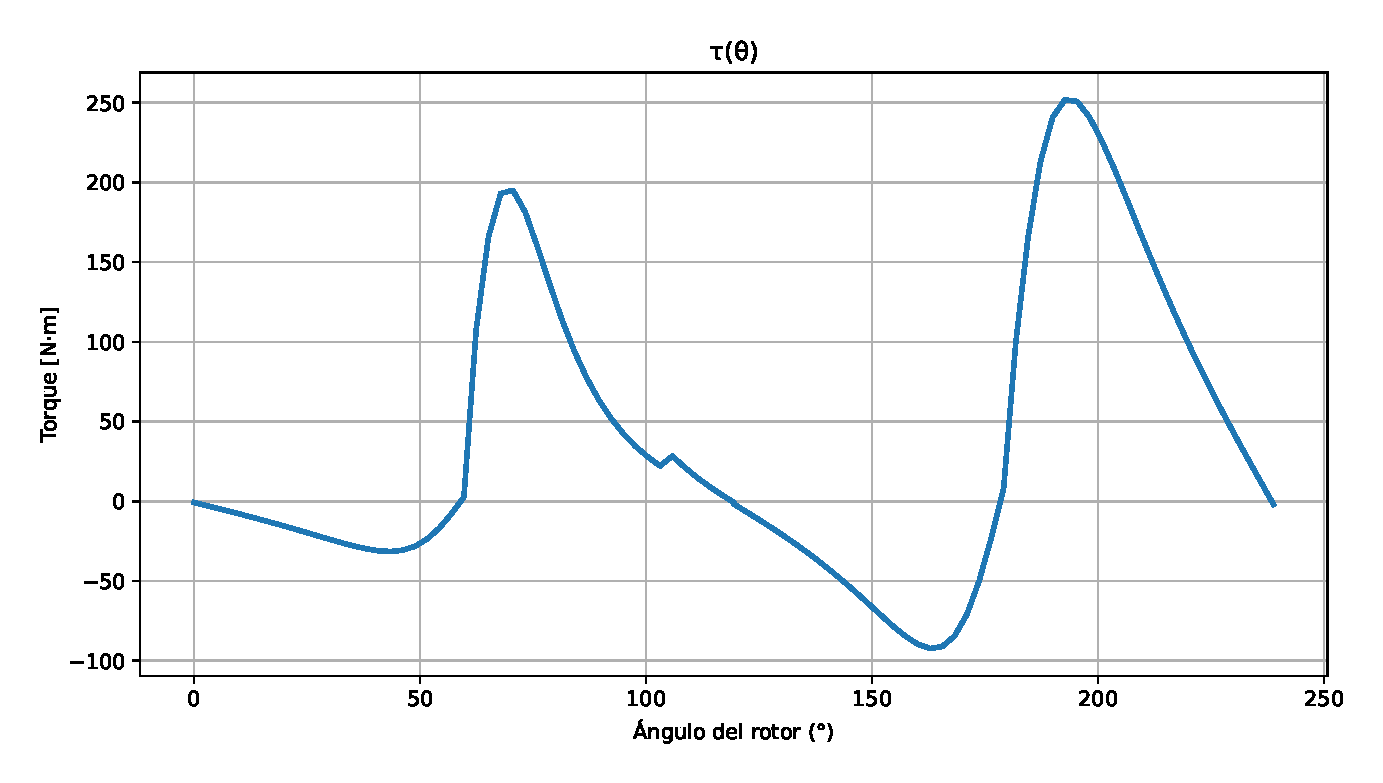
\includegraphics[width=0.6\textwidth]{torquesupch.eps}
    \caption{Torque de un ciclo \textbf{Caso A} (sobrealimentación con \emph{supercharger}) para el motor Wankel de seis tiempos. Fuente: elaboración propia}
    \label{fig:torque_p}
\end{figure}

En el caso con plenum, la Figura~\ref{fig:torque_p} muestra la evolución del torque a lo largo de un ciclo completo. El torque representa el momento de fuerza generado por la presión de los gases sobre las caras del rotor, siendo el vínculo directo entre la energía térmica de la combustión y la energía mecánica entregada al eje. 

El perfil presenta alternancias entre valores positivos y negativos: los negativos corresponden a las fases de compresión, donde la presión interna se opone al movimiento del rotor, y los positivos a las fases de expansión, en las que los gases ejercen trabajo útil. Se observan dos picos principales que se generan en el proceso isocórico, el primero cercano a 200~N·m y el segundo alrededor de 250~N·m. Este incremento en la segunda expansión se asocia con el aire presurizado del plenum, que eleva las condiciones de admisión y favorece una combustión más completa.


\begin{figure}[H]
    \centering
    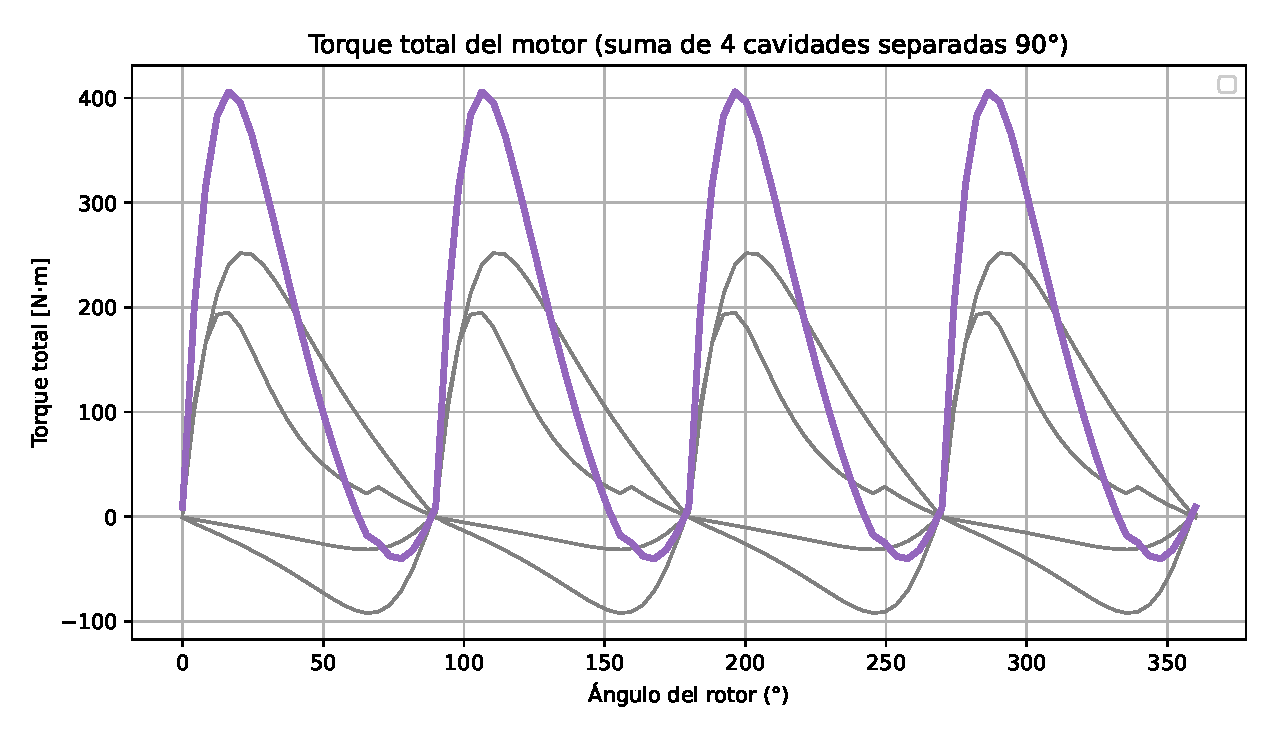
\includegraphics[width=0.6\textwidth]{torque4spch.eps}
    \caption{Torque del motor \textbf{Caso A} (sobrealimentación con \emph{supercharger}) para el motor Wankel de seis tiempos. Fuente: elaboración propia}
    \label{torquea}
\end{figure}


La Figura~\ref{torquea} presenta las cuatro curvas de torque correspondientes a cada una de las cámaras del rotor, desfasadas entre sí 90° para representar el funcionamiento secuencial del motor. Sobre ellas, la curva en color morado muestra la suma instantánea de los torques individuales, la cual corresponde al torque total entregado por el motor. Este torque combinado alcanza valores máximos superiores a 400~N·m y mínimos cercanos a −40~N·m. Se observa que durante la mayor parte del ciclo el torque resultante permanece en valores positivos, indicando que el motor entrega trabajo útil de forma continua. El valor promedio del torque total es de aproximadamente 150~N·m, lo que refleja un funcionamiento estable y una entrega sostenida de potencia a lo largo del ciclo completo.


\begin{figure}[H]
    \centering
    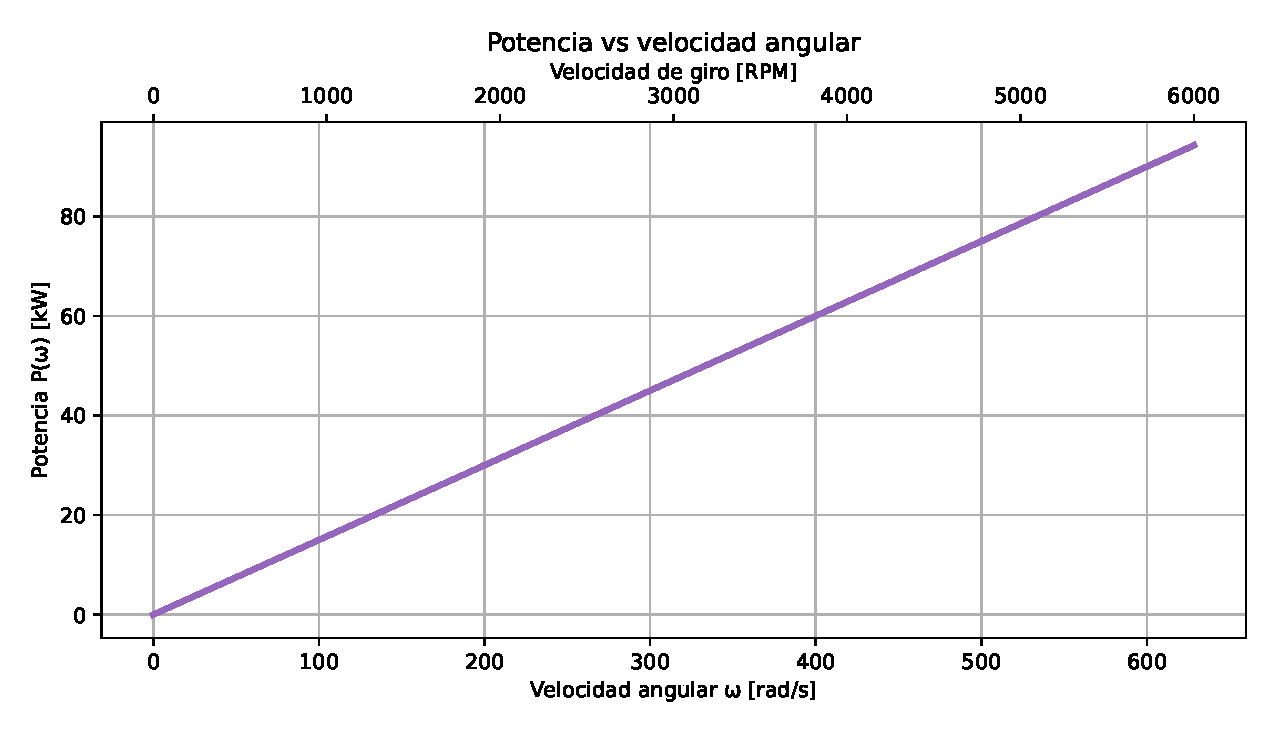
\includegraphics[width=0.6\textwidth]{potenciaspch.eps}
    \caption{Potencia nominal del \textbf{Caso A} (sobrealimentación con \emph{supercharger}) para el motor Wankel de seis tiempos. Fuente: elaboración propia}
    \label{psch}
\end{figure}

La Figura~\ref{psch} presenta la potencia nominal del motor en función de la velocidad angular, con el eje inferior en rad/s y el superior en revoluciones por minuto (rpm). La gráfica corresponde a una línea recta, resultado del cálculo directo mediante la ecuación \eqref{ptw} con un torque promedio constante de 150~N·m. Esta relación lineal refleja que la potencia aumenta proporcionalmente con la velocidad de giro, sin variaciones asociadas al ciclo, lo que permite visualizar de forma sencilla la capacidad del motor para generar trabajo mecánico a distintas velocidades.


\subsubsection{Termodinámica —(Caso B Inyección de agua)}

En esta sección se presentan los resultados del estudio de un motor con ciclo modificado de 6 tiempos con adición de 
agua.

\begin{figure}[H]
    \centering
    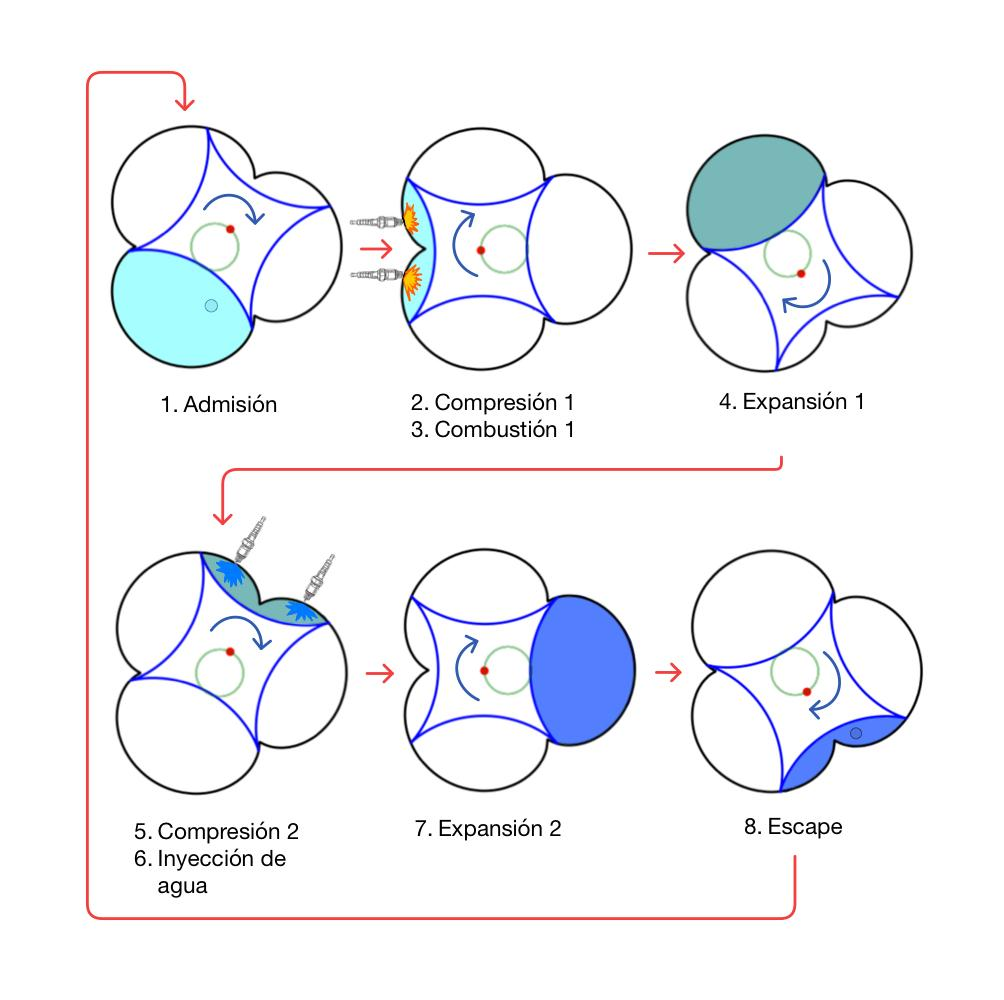
\includegraphics[width=0.55\textwidth]{agua.jpg}
    \caption{Diagrama de funcionamiento del \textbf{Caso B} (Inyección de \emph{agua}) para el motor Wankel de seis tiempos. Fuente: elaboración propia}
    \label{fig:pv_agua}
\end{figure}

La figura ilustra un ciclo de ocho etapas correspondiente a un motor Wankel de seis tiempos con inyección de agua. El proceso inicia con la admisión, seguida de la primera compresión y combustión, que generan la primera expansión. Después de esta fase, la cavidad entra en una segunda compresión durante la cual se realiza la inyección de agua, lo que incrementa la presión por vaporización del fluido. Este fenómeno origina una segunda expansión que aprovecha la energía adicional generada por el cambio de fase. Finalmente, el ciclo concluye con el escape de los productos resultantes antes de reiniciar la secuencia.

\begin{figure}[H]
    \centering
    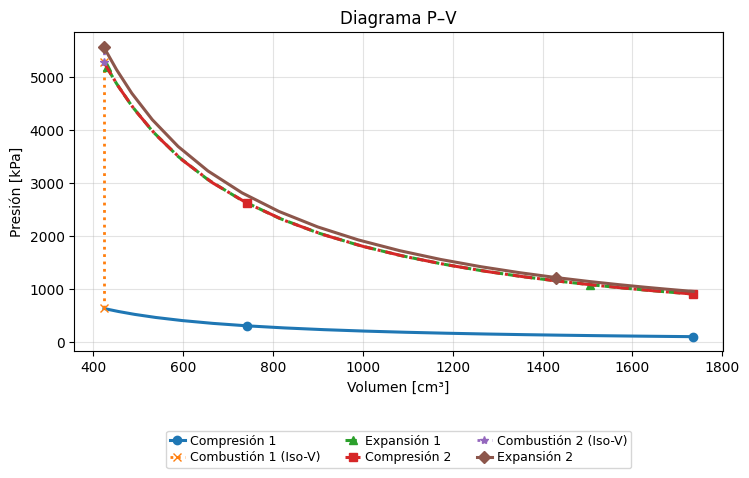
\includegraphics[width=0.65\textwidth]{pvaguagua.png}
    \caption{Diagrama $P$–$V$ del \textbf{Caso B} (Inyección de \emph{agua}) para el motor Wankel de seis tiempos. Fuente: elaboración propia}
    \label{fig:pv_agua}
\end{figure}


En este caso, las fases iniciales de compresión y combustión se desarrollan de forma similar a un motor Wankel convencional, siguiendo la ecuación politrópica~\eqref{eq:poly-base} y el proceso isocórico~\eqref{eq:isoV-base}. Durante la primera combustión se adicionan \(5.63~\text{kJ}\) de calor, alcanzando una presión máxima de \(5287.30~\text{kPa}\) y una temperatura máxima de 3820,10 K en un volumen de \(423.26~\text{cm}^3\). La primera expansión libera \(2.36~\text{kJ}\) de trabajo, completando la primera parte del ciclo P–V.  

Luego, en el volumen mínimo, se inyecta agua aprovechando la alta temperatura de los gases residuales. Esta se evapora instantáneamente (\(1.139~\text{g}\)), con un aporte térmico de \(5.30~\text{kJ}\) elevando la presión a 5670,0 kPa y disminuyendo la temperatura a 2292,05 K. El proceso ocurre sobre la misma línea politrópica de la primera expansión, ya que no hay liberación de gases y la energía interna se transfiere al agua; el trabajo resultante es equivalente en magnitud pero de signo opuesto. La segunda expansión genera \(2.81~\text{kJ}\), obteniéndose un trabajo neto de \(2.50~\text{kJ}\), lo que evidencia la contribución positiva de la vaporización al rendimiento del ciclo.  

El calor total introducido fue \(Q_{\text{in}} = 5.63~\text{kJ}\) (sin considerar el aporte externo de \(5.30~\text{kJ}\)), y la eficiencia térmica alcanzó \(\eta = 44.40\%\), demostrando una mejor utilización del calor residual al convertir parte del calor latente en trabajo útil.










\begin{figure}[H]
    \centering
    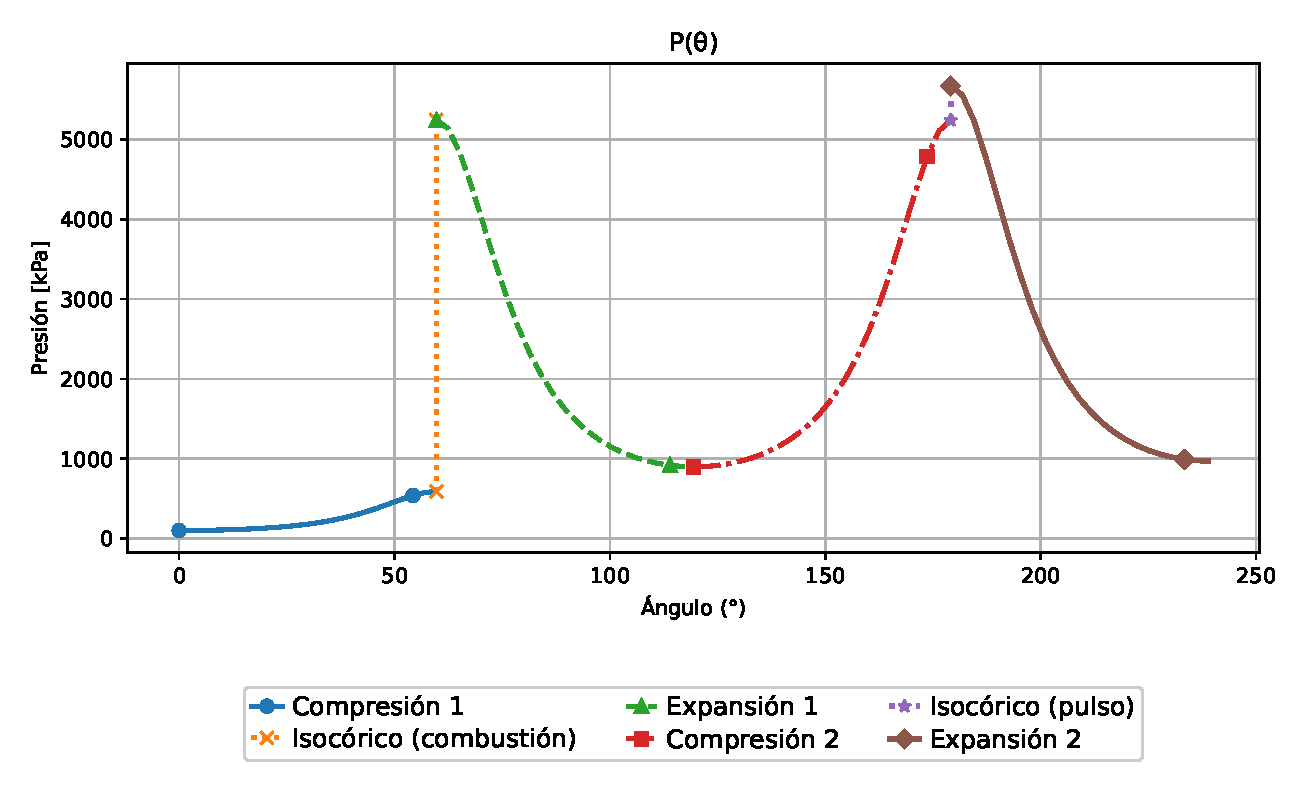
\includegraphics[width=0.7\textwidth]{aguapresion.eps}
    \caption{Presión con relación al angulo del rotor \textbf{Caso B} (Inyección de \emph{agua}) para el motor Wankel de seis tiempos. Fuente: elaboración propia}
    \label{Pagua}
\end{figure}

La Figura~\ref{Pagua} presenta la variación de la presión con respecto al ángulo de rotación del rotor. A diferencia de los demás casos se observa que los procesos de expansión 1 y compresión 2 presentan valores idénticos pero en sentidos opuestos, evidenciando la simetría entre ambas fases que se comentó previamente en la gráfica P-V. También, se aprecia el aumento de presión generado durante el segundo proceso isocórico de adición de agua, que inicia en 5284~kPa en el cual la presión alcanza un valor máximo aproximado de 5670~kPa, antes de dar inicio a la segunda expansión que completa el ciclo.


\begin{figure}[H]
    \centering
    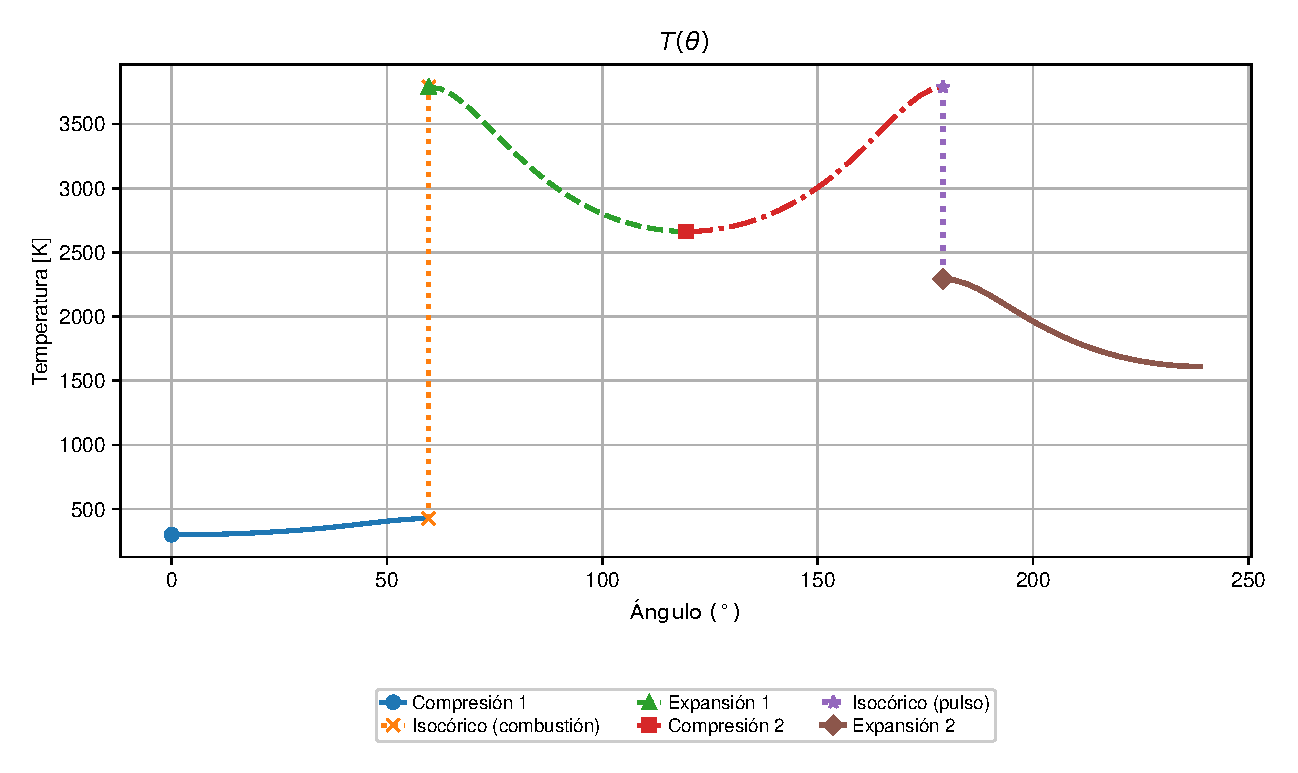
\includegraphics[width=0.7\textwidth]{aguatempp.eps}
    \caption{Temperatura con relación al angulo del rotor \textbf{Caso B} (Inyección de \emph{agua}) para el motor Wankel de seis tiempos. Fuente: elaboración propia}
    \label{fig:temperatura_angulo}
\end{figure}

La Figura~\ref{fig:temperatura_angulo} presenta la variación de la temperatura en función del ángulo de rotación del rotor. Las primeras fases se desarrollan de manera convencional, como en un motor Wankel típico. Durante la primera expansión, la temperatura disminuye gradualmente a medida que los gases realizan trabajo sobre el rotor, habiendo alcanzado previamente un valor máximo de aproximadamente \(3780~\text{K}\) durante la primera combustión. Posteriormente, se observa que la temperatura vuelve a alcanzar un valor similar tras el segundo proceso isocórico asociado a la inyección de agua. A continuación, se produce un descenso notable de la temperatura, en contraste con el aumento de presión registrado en la misma etapa. Este comportamiento se explica porque el agua inyectada absorbe una fracción significativa del calor interno durante su vaporización, lo que reduce la energía térmica disponible en la cámara y estabiliza las condiciones antes del inicio de la segunda compresión.




\begin{figure}[H]
    \centering
    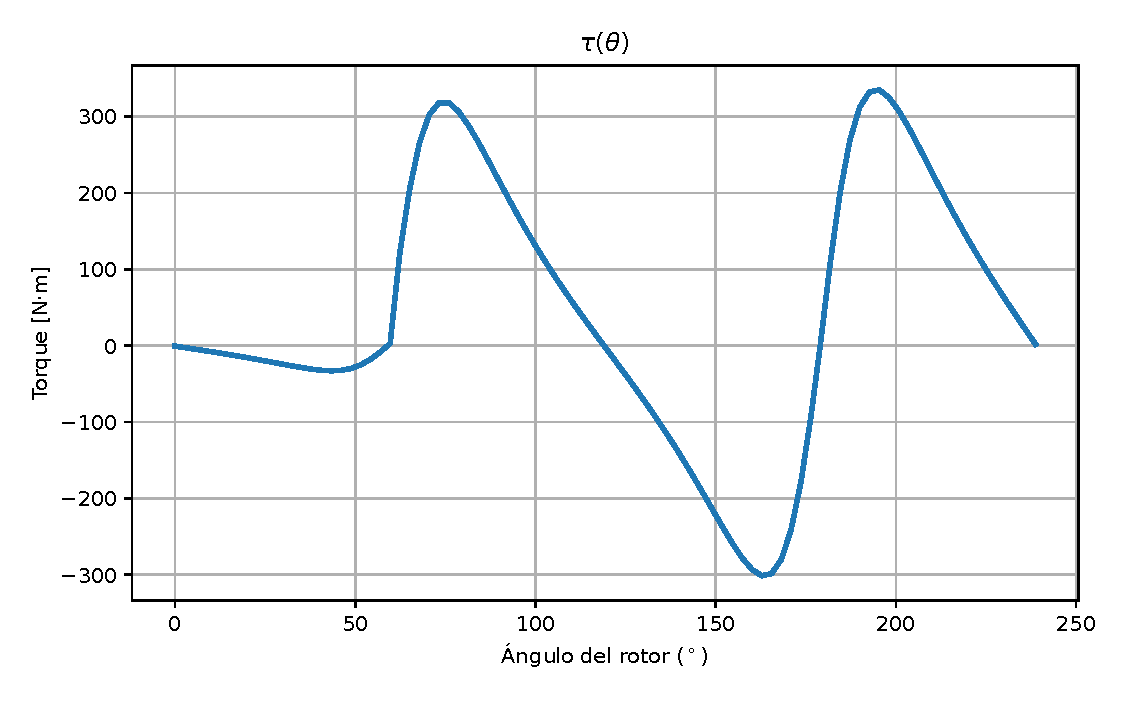
\includegraphics[width=0.6\textwidth]{torqueagua.eps}
    \caption{Torque de un ciclo  \textbf{Caso B} (Inyección de \emph{agua}) para el motor Wankel de seis tiempos. Fuente: elaboración propia}
    \label{Torqueag}
\end{figure}

En la figura \ref{Torqueag} como en las anteriores gráficas refeleja el comportamiento simétrico entre la primera expansión y la segunda compresión donde el torque alcanza un máximo de 310 N.m de torque posterior al proceso isocórico y su valor mínimo al completar la compresión 2 de -300 N.m y finalmente alcanza el valor máximo de 327 N.m luego de la adición de calor 2

\begin{figure}[H]
    \centering
    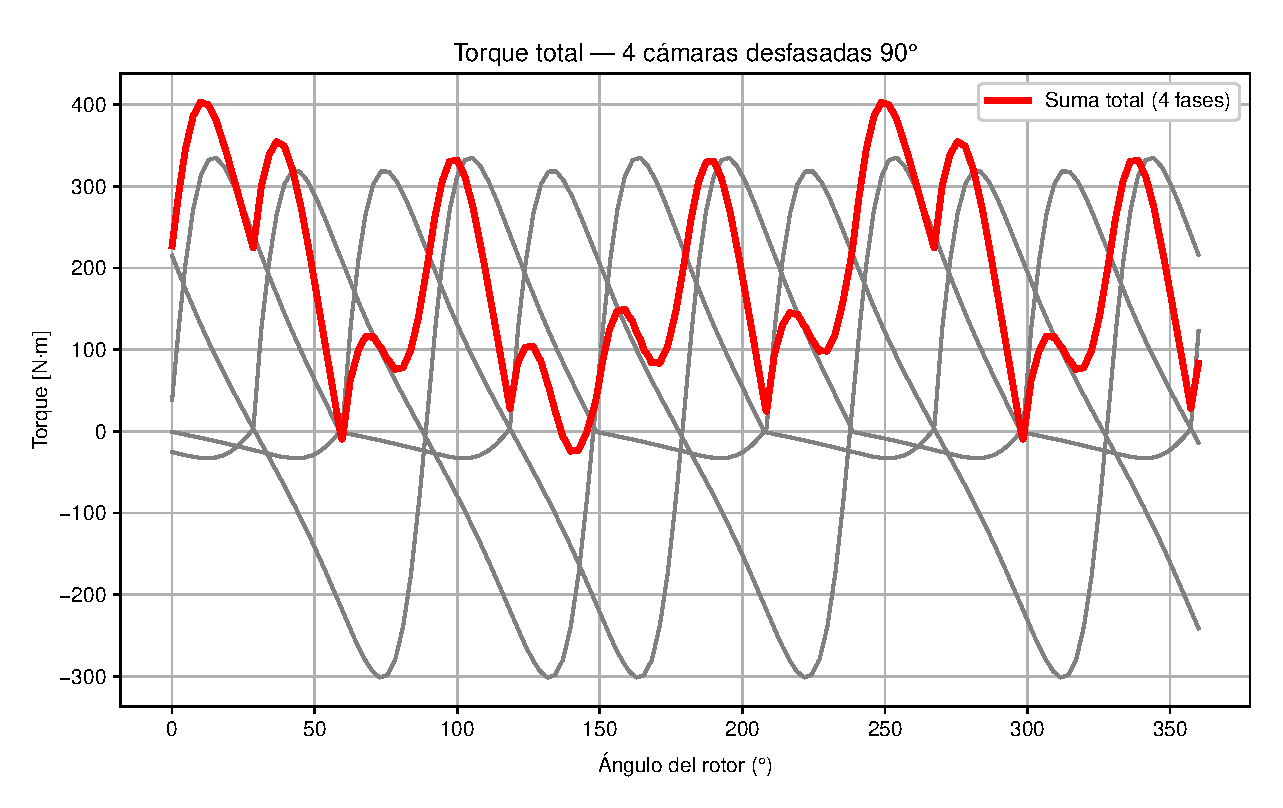
\includegraphics[width=0.6\textwidth]{torquetotalagua.eps}
    \caption{Torque del motor  \textbf{Caso B} (Inyección de \emph{agua}) para el motor Wankel de seis tiempos. Fuente: elaboración propia}
    \label{torquemag}
\end{figure}

El torque del motor se presenta en la figura \ref{torquemag} donde se observa la suma de los torques generados para cada angulo del rotor presentados en gris, tomando en cuenta todas las cavidades que se ubican en intervalos de 90°. El torque da un promedio de 189.5 N·m con valores máximo y minimo de 402.8 N·m y -24.5 N.m

\begin{figure}[H]
    \centering
    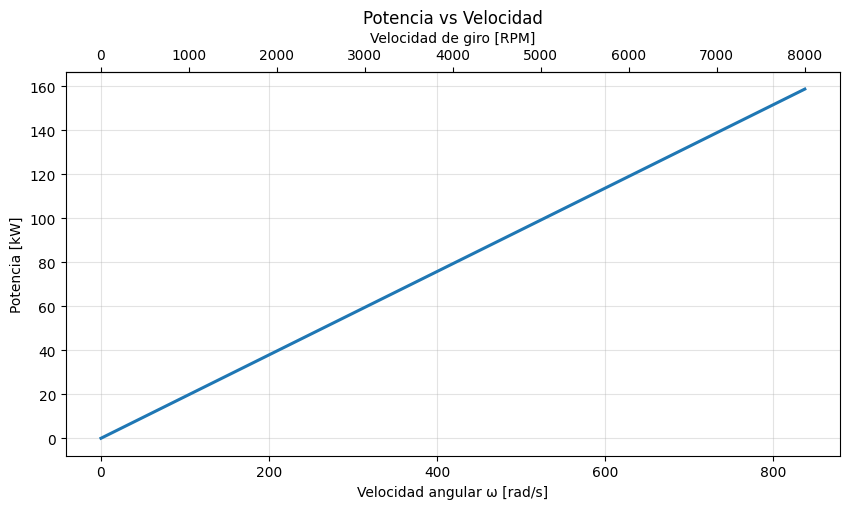
\includegraphics[width=0.6\textwidth]{potenciaaguagua.png}
    \caption{Potencia nominal del motor  \textbf{Caso B} (Inyección de \emph{agua}) para el motor Wankel de seis tiempos. Fuente: elaboración propia}
    \label{pagua}
\end{figure}


La Figura~\ref{pagua} muestra la potencia del motor en función de la velocidad angular, con ejes en rad/s y rpm. La relación lineal obtenida a partir de la ecuación~\eqref{ptw}, usando un torque promedio constante de 189.5~N·m, evidencia que la potencia crece proporcionalmente con la velocidad de giro, reflejando la capacidad del motor para generar trabajo mecánico de forma estable.





\subsubsection{Termodinámica —(Caso C Valvula)}

En esta sección se presentan los resultados del estudio de un motor con ciclo modificado de 6 tiempos con una valvula de expansión 

\begin{figure}[H]
    \centering
    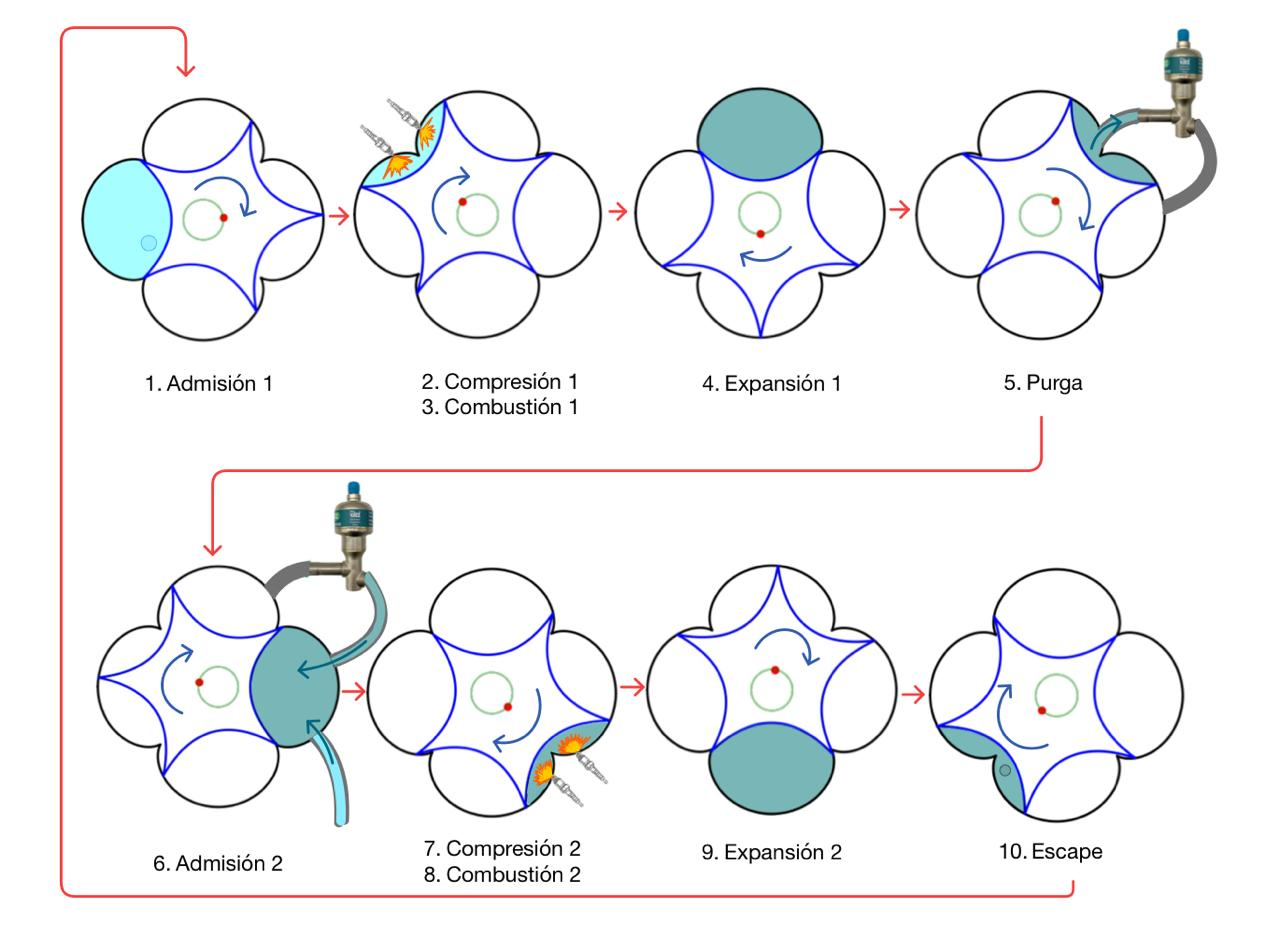
\includegraphics[width=0.6\textwidth]{Valvula de exp.jpg}
    \caption{Diagrama de funcionamiento del \textbf{Caso C} Válvula de expansión para el motor Wankel de seis tiempos. Fuente: elaboración propia}
    \label{fig:motor_casoA}
\end{figure}

La figura representa un ciclo de diez etapas correspondiente a un motor Wankel de seis tiempos con un sistema de purga y admisión mediante válvula de expansión. El proceso comienza con la primera admisión, seguida por la compresión y combustión iniciales que generan la primera expansión. Una vez liberada esta energía, se activa una fase de purga que evacúa los gases residuales antes de iniciar la segunda etapa de llenado. Durante la segunda admisión, la válvula incorpora aire fresco directamente hacia la cavidad activa, lo que permite una posterior compresión y la segunda combustión. Esto produce una segunda expansión que aprovecha la energía adicional generada en esta etapa. Finalmente, los productos de combustión se evacuan en la fase de escape, cerrando el ciclo ampliado de seis tiempos.

\begin{figure}[H]
    \centering
    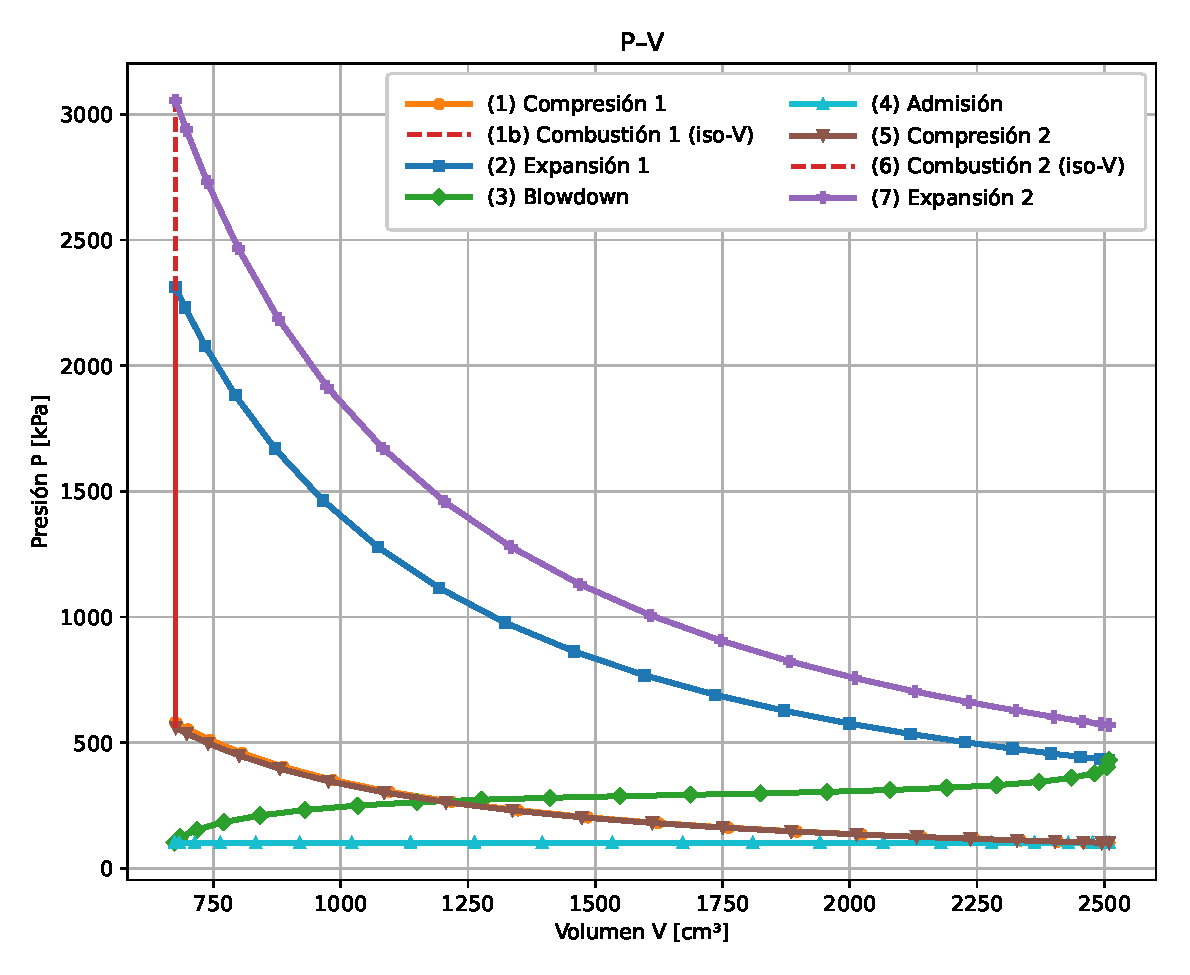
\includegraphics[width=0.6\textwidth]{imagenes/PV_completo_versionfinal.eps}
    \caption{Diagrama $P$–$V$ del \textbf{Caso C} Válvula de expansión para el motor Wankel de seis tiempos. Fuente: elaboración propia}
    \label{fig:motor_casoA}
\end{figure}


En este caso, las fases de compresión, combustión y expansión siguen las ecuaciones~\eqref{eq:poly-base}, \eqref{eq:isoV-base} y nuevamente~\eqref{eq:poly-base}. A diferencia de un motor de cuatro tiempos, los gases de escape no se liberan al ambiente, sino que pasan por una válvula de expansión que reduce su presión hasta niveles cercanos al atmosférico.  

Este proceso se modeló mediante la ecuación~\eqref{eq:dm-dtheta}. Durante la admisión, ingresan simultáneamente aire fresco y gases recirculados, ambos a presión atmosférica. Se asumió una presión constante, pues la válvula de admisión permanece abierta y el colector mantiene una presión casi invariable, por lo que las variaciones de volumen no alteran significativamente la presión del gas admitido.  

Luego ocurre una compresión politrópica seguida de la combustión, alcanzándose presiones elevadas según~\eqref{eq:isoV-base}, dependientes de la temperatura. Los gases recirculados entran a \(1163~\text{K}\) y llegan a \(1725~\text{K}\) al final de la compresión; según~\eqref{eq:EOS-bd}, este aumento térmico genera presiones altas. El ciclo finaliza con una expansión normal.  

El balance energético considera \( Q_{\text{rel,C1}} = 2.93~\text{kJ} \) y \( Q_{\text{rel,C2}} = 1.23~\text{kJ} \), sumando \( Q_{\text{in}} = 4.16~\text{kJ} \). A partir de~\eqref{eq:Trabajo_Neto} se obtiene \( W_{\text{net}} \) y una eficiencia térmica de \( \eta_t = 67.99~\% \), que evidencia un aprovechamiento notable del calor liberado y la efectividad de la válvula de expansión para recuperar energía de los gases y uHC antes de su liberación.




\begin{figure}[H]
    \centering
    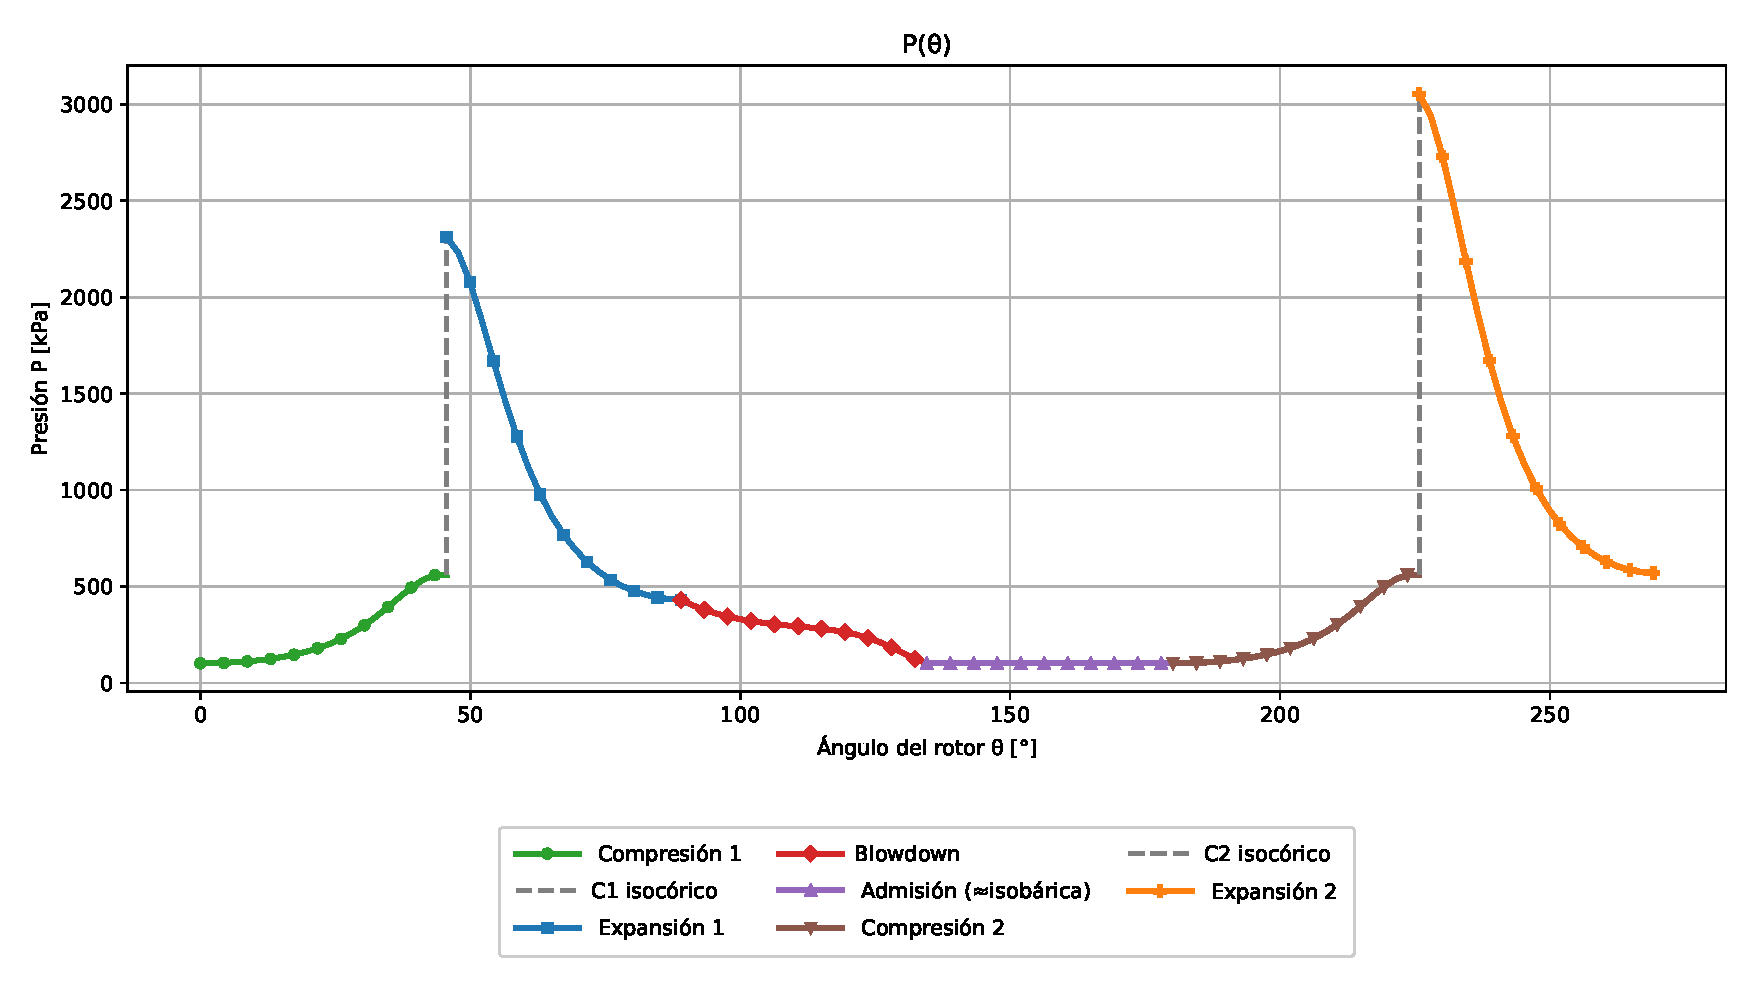
\includegraphics[width=0.7\textwidth]{imagenes/P_vs_theta_6T_exp2_integrado_versionfinal.eps}
    \caption{Diagrama \( P(\theta) \) del \textbf{Caso C} (Vávula) para el motor Wankel de seis tiempos. Fuente: elaboración propia}
    \label{fig:motor_casoA}
\end{figure}


Se observa que la presión posterior a la combustión 2 ( \(3054.38 ~\text{kPa}\)) es superior a la alcanzada después de la combustión 1  (\(2312.6~\text{kPa}\)). Esto ocurre debido a que los gases de escape, al ingresar calientes, transfieren parte de su energía térmica al aire fresco, elevando así la temperatura total de la mezcla dentro de la cámara. El aire caliente contribuye con energía térmica adicional, la cual se convierte en energía de presión y posteriormente en trabajo mecánico durante el ciclo. Como resultado, el incremento relativo de temperatura y presión durante la compresión 2 es moderado, pero el proceso de combustión logra alcanzar presiones absolutas más elevadas sin requerir un trabajo de compresión considerablemente mayor.



\begin{figure}[H]
    \centering
    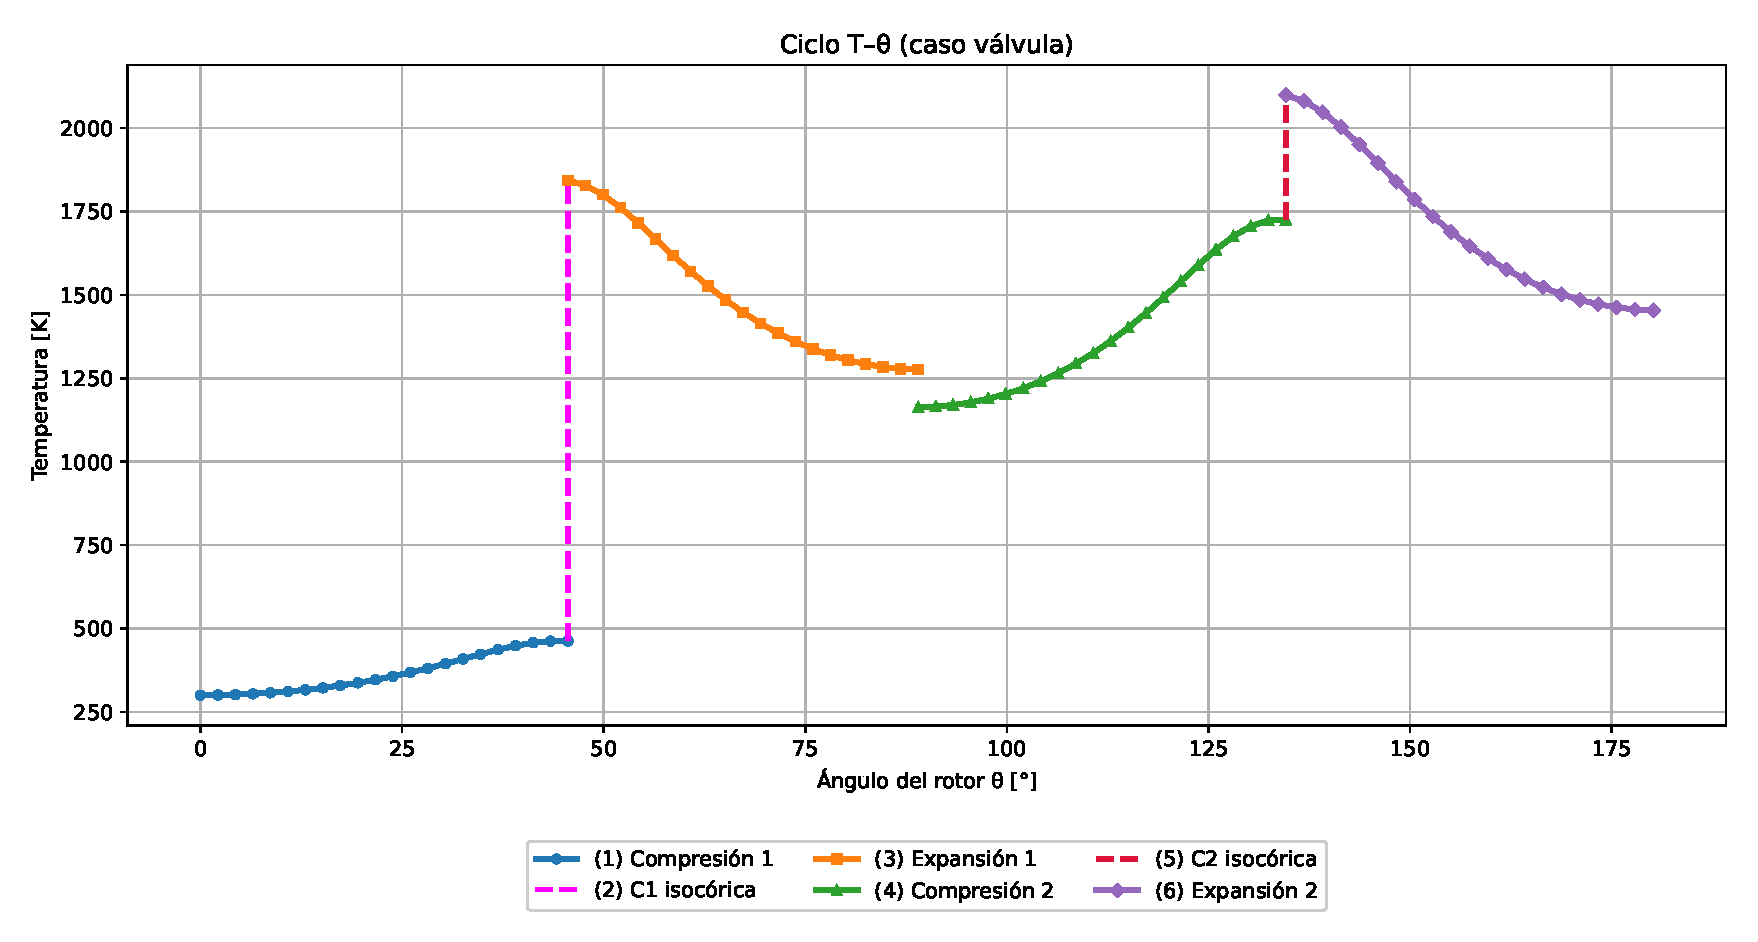
\includegraphics[width=0.7\textwidth]{imagenes/T_vs_theta_ciclo_completo_valvula_versionfinal.eps}
    \caption{Diagrama \( T(\theta) \)
 del \textbf{Caso C} (Vávula) para el motor Wankel de seis tiempos. Fuente: elaboración propia}
    \label{fig:motor_casoA}
\end{figure}


Se observa el fenómeno mediante el cual los gases calientes generados durante la compresión y la combustión en el interior de la cámara del motor son aprovechados antes de su expulsión. Dado que los gases de escape presentan temperaturas considerablemente elevadas, al atravesar una válvula de expansión su presión disminuye sin que la temperatura experimente una variación significativa. Al ser recirculados, este proceso permite recuperar parte del calor residual para precalentar el aire fresco antes de la fase de compresión, incrementando así su temperatura inicial. En consecuencia, la fase de admisión se encuentra a un nivel térmico superior al de la fase inicial de la compresión 1, lo que favorece la obtención de presiones más altas a lo largo del ciclo termodinámico. Finalmente, el salto observado entre la fase de blowdown y la admisión se debe a la mezcla entre los gases calientes de escape, con una temperatura aproximada de \(1275.81~\text{K}\), y el aire fresco admitido a \(300~\text{K}\).



\begin{figure}[H]
    \centering
    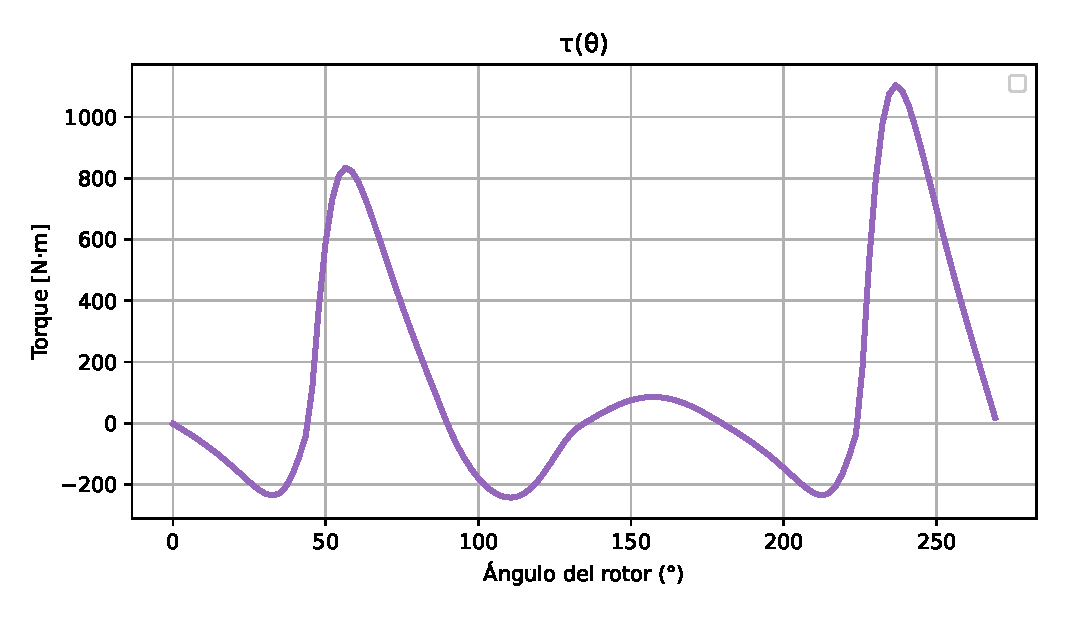
\includegraphics[width=0.7\textwidth]{torquevexp.eps}
    \caption{Diagrama \( \(\tau \)(\theta) \)
 del \textbf{Caso C} (Vávula) para el motor Wankel de seis tiempos. Fuente: elaboración propia}
    \label{torqueval}
\end{figure}}

La figura \ref{torqueval} muestra el comportamiento del torque en una cavidad para cada angulo del rotor y se observan tres minimos para las 3 compresiones oscilando valores menores a -200 N.m, asi como 2 máximoss para las adiciones de calor, alcanzando valores de 813 N.m en la primera adición de calor y de 1100 N.m para la segunda. Los valores de torque de este motor son mayores ya que el brazo r en el que se aplica la fuerza es también mayor

\begin{figure}[H]
    \centering
    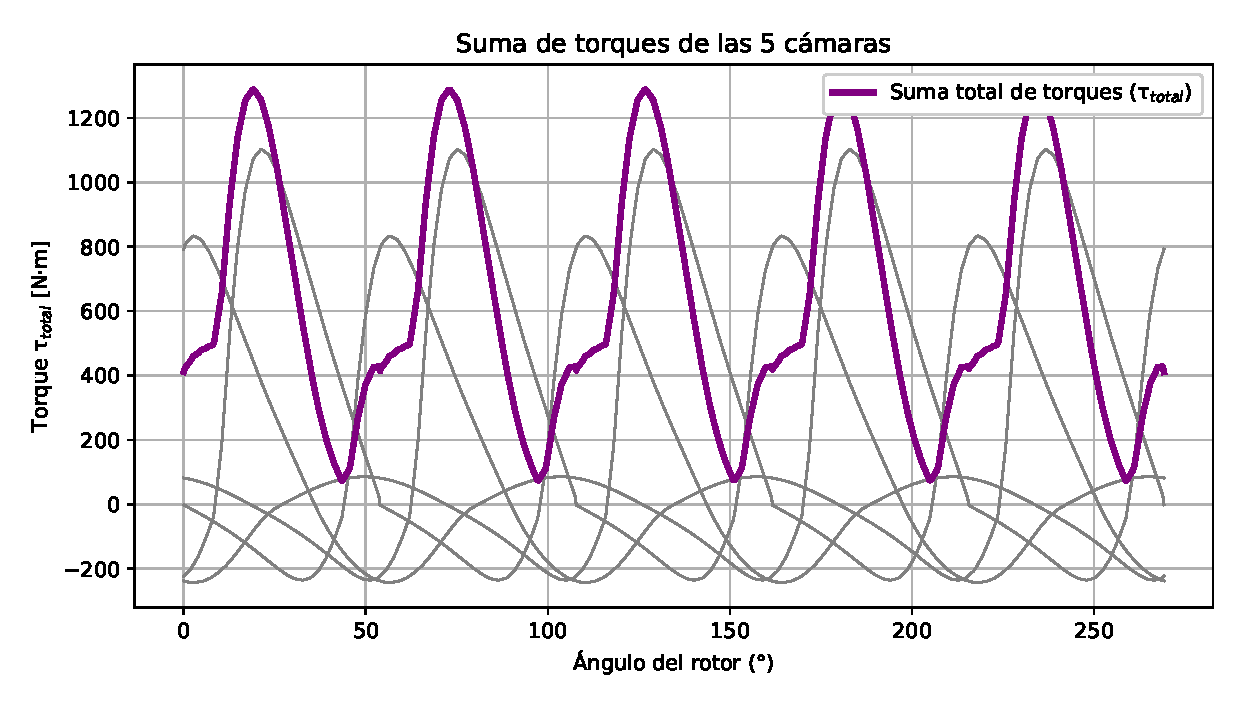
\includegraphics[width=0.7\textwidth]{suma_total_torques.eps}
    \caption{Diagrama \( \(\tau \)(\theta) del motor\)
 del \textbf{Caso C} (Vávula) para el motor Wankel de seis tiempos. Fuente: elaboración propia}
    \label{5tv}
\end{figure}

En la figura \ref{5tv} se muestran las 5 curvas de torque desfasadas que ocurren al mismo angulo en gris y la gráfica de la suma de todas, este es el torque que produce el motor que en promedio genera 626.5 N.m de torque con valores máximo y minimo de 1289 N.m y 95 N.m.



\begin{figure}[H]
    \centering
    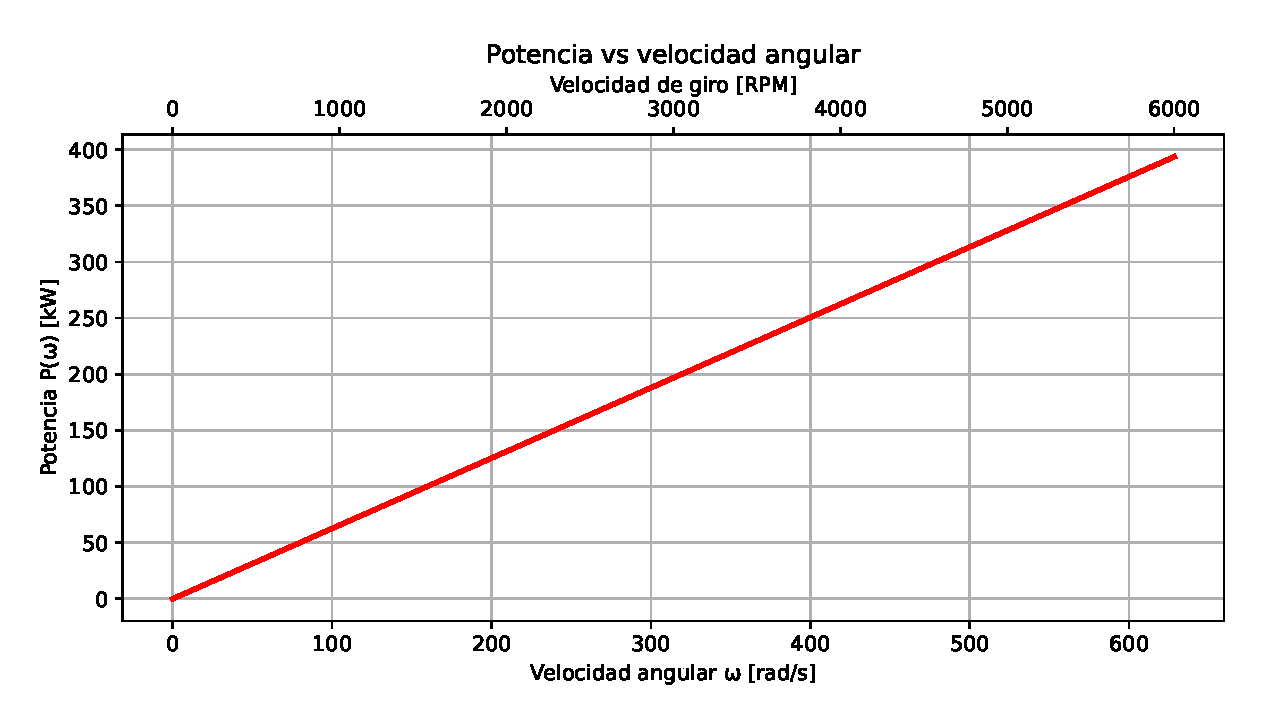
\includegraphics[width=0.7\textwidth]{potenciavalv.eps}
    \caption{Potencia nomimal 
 del motor \textbf{Caso C} (Vávula) para el motor Wankel de seis tiempos. Fuente: elaboración propia}
    \label{fig:motor_casoA_potencia}
\end{figure}

En esta figura se observa una gráfica teorica de la potencia nominal del motor con un torque promedio de 626.459 N.m 
  

\subsection{Comparación entre el Motor Wankel de Seis Tiempos y el de Cuatro Tiempos}

A continuación se presentan las gráficas del motor Wankel de cuatro tiempos comparadas con los tres casos del motor Wankel de seis tiempos. El criterio de comparación exige que ambos motores, independientemente de su geometría, posean el mismo volumen máximo y la misma relación de compresión. Se fijaron \(V_{\max} = 1735.3~\text{cm}^3\) y \(r_c = 4.1\), a partir de los cuales se calcularon los parámetros geométricos mostrados en la Tabla~\ref{tab:param_geom_motor}. Con estos valores se garantizó la equivalencia entre configuraciones.  

Los modelos de cuatro tiempos y seis tiempos con válvula de expansión fueron ajustados, pues inicialmente no cumplían dichas condiciones. Se modificaron sus parámetros geométricos y se generaron nuevamente las curvas de volumen–ángulo, presión–volumen (P–V) y potencia–RPM, bajo los mismos criterios de comparación. En el caso del motor de seis tiempos con válvula, las restricciones geométricas impidieron igualar exactamente los valores objetivo. Se obtuvo un volumen máximo de \(1734.82~\text{cm}^3\) y una relación de compresión de \(3.73\), considerados suficientemente cercanos para efectos comparativos.  

A continuación se presentan las gráficas finales de cada configuración.




\begin{figure}[H]
    \centering
    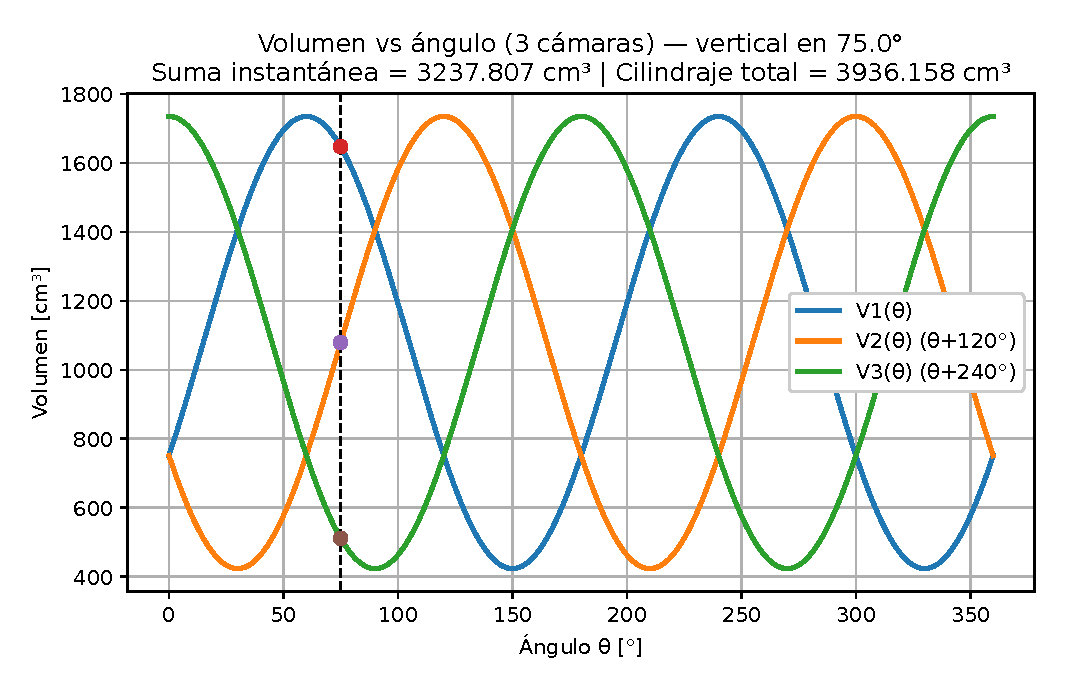
\includegraphics[width=0.55\textwidth]{imagenes/volumen_3camaras_vertical_y_suma.eps}
    \caption{Gráfica de volumen vs angulo del Motor Wankel de 4 tiempos. Fuente: elaboración propia}
    \label{fig:4tiempos_vol_3camaras}
\end{figure}


En comparación con el motor de cuatro tiempos de tres cámaras, con un cilindraje de \(V_d = 3936.158~\text{cm}^3\), el motor de seis tiempos con cuatro cámaras (\ref{fig:4fases_3lob}) incrementa el desplazamiento a \(5248.143~\text{cm}^3\) (\(+33.33\,\%\)). El de seis tiempos con válvula y cinco cámaras  alcanza \(6346.044~\text{cm}^3\), es decir, un (\(+61.22\,\%\)) frente al 4T y un (\(+20.92\,\%\)) respecto al de cuatro cámaras.  

A igualdad de IMEP y régimen, un mayor \(V_d\) implica una mayor potencia indicada. Por ello, el 6T con válvula ofrece la mayor capacidad de entrega y, al contar con más cámaras activas, logra una suma volumétrica instantánea más continua, traduciéndose en un par más uniforme. Aunque su relación de compresión es ligeramente menor (\(r_c \approx 3.73\)) frente a \(4.10\) de los demás motores, el aumento de desplazamiento y la multiplicidad de eventos de trabajo compensan esta diferencia y mejoran el desempeño global.  



\begin{figure}[H]
    \centering
    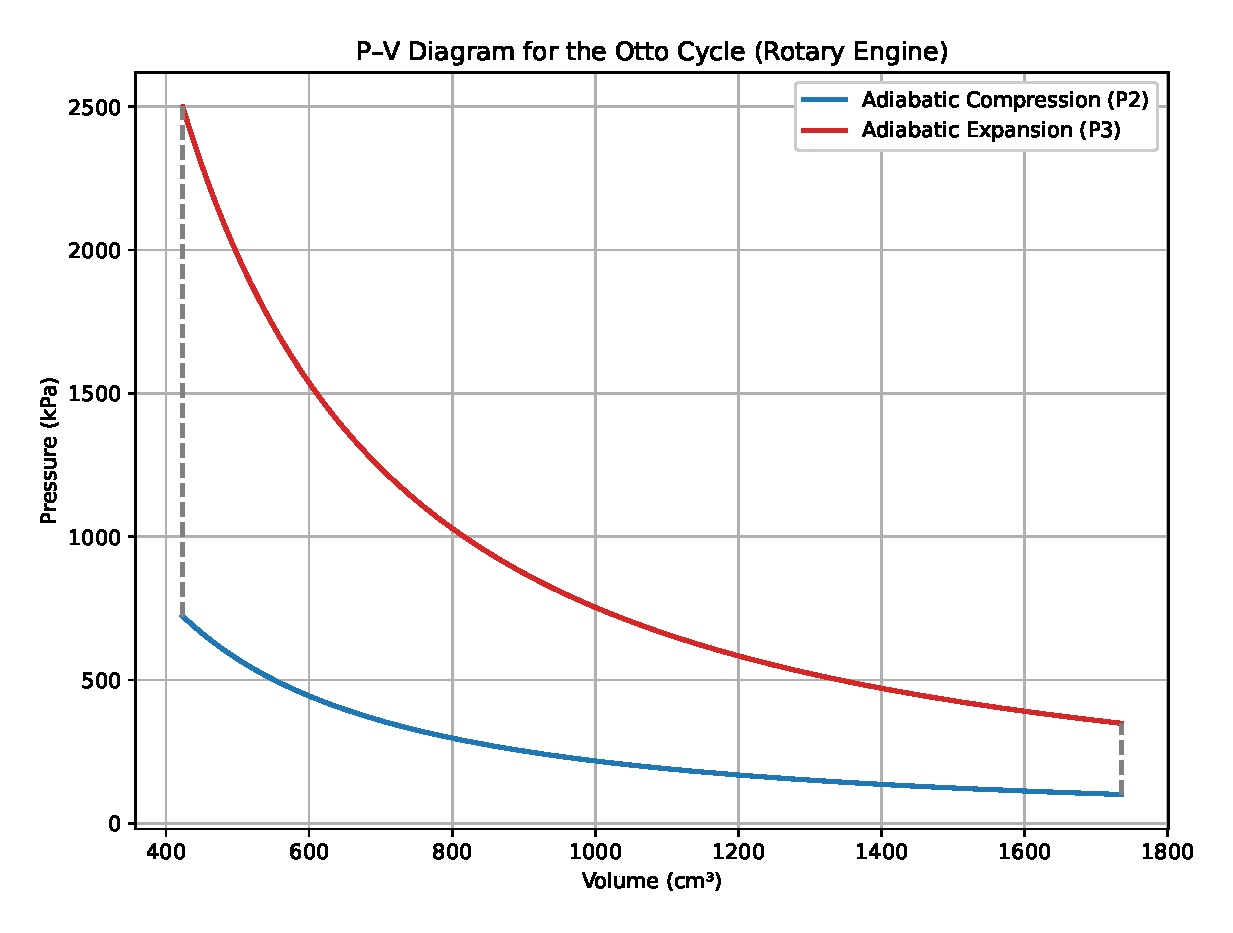
\includegraphics[width=0.65\textwidth]{PV_diagram_version_final.eps}
    \caption{P-V o del motor Wankel 4 tiempos. Fuente: elaboración propia}
    \label{fig:4tiempos_PV}
\end{figure}

Las Figuras~(\ref{fig:4tiempos_PV}), (\ref{fig:motor_casoA}) y~(\ref{fig:pv_agua}) presentan las curvas \(P\)-\(V\) del motor de cuatro tiempos y de los motores de seis tiempos con válvula expansiva, supercargador e inyección de agua. En el caso del motor con válvula, la simulación se ejecutó utilizando los criterios de relación de compresión y volumen máximo establecidos en la sección previa. A partir de estas curvas se calcularon el trabajo por ciclo, el calor de entrada y la eficiencia térmica, parámetros fundamentales para la comparación entre configuraciones.

\begin{table}[H]
\centering
\caption{Métricas indicadas a partir de las curvas P–V.}
\label{tab:pv_metrics}
\begin{tabular}{lcccc}
\toprule
Magnitud & 4T & 6T (supercargador) & 6T (agua) & 6T (con válvula) \\
\midrule
$V_{\max}$ [cm$^3$] & 1735.30 & 1735.30 & 1735.30 & 1734.82 \\
Relación de compresión $r_c$ & 4.10 & 4.10 & 4.10 & 3.73 \\
Trabajo indicado por ciclo $W_i$ [kJ] & \textbf{1.323} & \textbf{4.562} & \textbf{2.50} & \textbf{2.840} \\
Calor de entrada $Q_{in}$ [kJ] & $4.28$ & $8.960$ \,( $5.710+3.250$) & $5.63$ & $4.160$ \,( $2.930+1.230$) \\
Eficiencia indicada $\eta_i$ [\%] & \textbf{30.91} & \textbf{50.91} & \textbf{44.40} & \textbf{68.28} \\
\bottomrule
\end{tabular}
\label{tabla}
\end{table}

En orden descendente de eficiencia, el comportamiento de los motores fue el siguiente: motor de seis tiempos con válvula expansiva (68.28~\%), motor de seis tiempos con supercargador (50.91~\%), motor de seis tiempos con inyección de agua (44.40~\%) y motor de cuatro tiempos (30.91~\%). El motor de seis tiempos con válvula resultó ser el más eficiente, generando un trabajo de 2.84~kJ con el menor aporte de calor (4.16~kJ), gracias al aprovechamiento de la energía contenida en los gases residuales durante la compresión y a la inclusión de una segunda combustión controlada.  

Por su parte, el motor de seis tiempos con supercargador alcanzó el mayor trabajo indicado (4.562~kJ), aunque con una eficiencia inferior a la del sistema con válvula, debido al mayor calor suministrado (8.96~kJ). Esta diferencia se explica por la reducción del AFR, que permitió inyectar una mayor cantidad de combustible durante la admisión y posibilitó una segunda combustión.  

En cuanto al motor de seis tiempos con inyección de agua, con un trabajo de 2.50~kJ y una eficiencia del 44.40~\%, presentó un comportamiento intermedio. La inyección de agua contribuyó a estabilizar la temperatura del ciclo, aunque limitó la recuperación energética, ya que la vaporización del agua absorbió una fracción significativa del calor liberado en la cámara, sin involucrar una segunda combustión.  

Finalmente, el motor de cuatro tiempos, con un trabajo de 1.323~kJ y un calor de entrada de 4.28~kJ, fue el menos eficiente al poseer una única combustión y carecer de mecanismos de recuperación térmica. Cabe resaltar que, si bien todos los casos emplearon isooctano como combustible, únicamente los motores con válvula expansiva y con supercargador efectuaron dos combustiones, lo que justifica sus mayores rendimientos globales.


 

\begin{figure}[H]
    \centering
    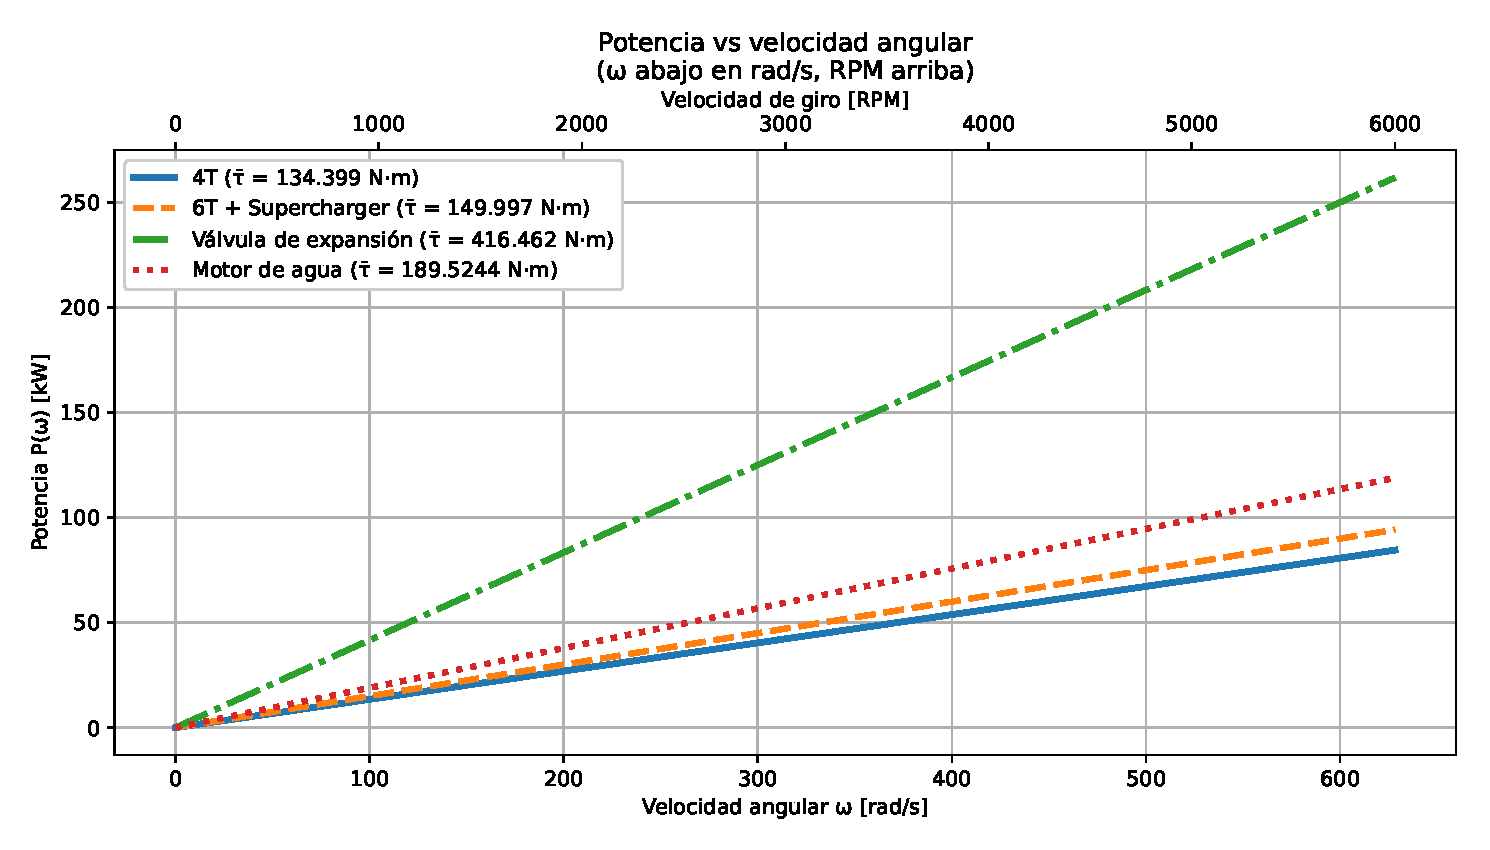
\includegraphics[width=0.7\textwidth]{imagenes/potencia_vs_omega_y_rpm_4curvas.eps}
    \caption{Gráfica de presión vs angulo del Motor Wankel de 4 tiempos. Fuente: elaboración propia}
    \label{Potencia4mots}
\end{figure}

La figura \ref{Potencia4mots} muestra la potencia nominal de los 4 motores estudiados 

La gráfica evidencia que el motor de seis tiempos con válvula alcanza la mayor potencia nominal (aproximadamente 270~kW a 6000~RPM), impulsado por su alto torque promedio (416.46~N·m) y la recuperación de energía en la segunda combustión. Le siguen el motor con agua (120~kW, 189.52~N·m) y el supercargador (90~kW, 150~N·m), cuyos rendimientos intermedios se deben al enfriamiento del ciclo y a la sobrealimentación, respectivamente. El motor de cuatro tiempos presenta la menor potencia (134.40~N·m) por carecer de procesos de recuperación. En todos los casos, la potencia crece linealmente con la velocidad angular.





\section{Componente de Dise\~no en Ingenier\'ia}



\subsection{Declaración y proceso de diseño}

El diseño desarrollado en este proyecto corresponde a una herramienta computacional implementada en Python para la simulación del comportamiento termo–mecánico de un motor rotativo tipo Wankel de seis tiempos. La finalidad de esta herramienta es modelar con precisión los fenómenos físicos asociados a cada una de las fases del ciclo, permitiendo analizar la evolución de la presión, la temperatura, el volumen y el torque a lo largo de la rotación del rotor. De esta manera, la propuesta trasciende la conceptualización teórica y se materializa en un entorno de simulación capaz de reproducir digitalmente el funcionamiento de una arquitectura rotativa no convencional.

El proceso de diseño se estructuró en módulos funcionales dentro del entorno Google Colab, que permitieron desarrollar y ejecutar de manera integrada los cálculos geométricos y termodinámicos. El módulo geométrico incluyó dos motores de seis tiempos, uno con estator de tres lóbulos y otro con estator de cuatro lóbulos, basados en las relaciones cinemáticas y volumétricas descritas en la sección 3.2. A partir de los resultados de volumen, el módulo termodinámico resolvió los procesos politrópicos e isocóricos de cada etapa del ciclo, generando las curvas de presión, temperatura y torque asociadas a cada ángulo de rotación. Este bloque imprimió los resultados en forma de gráficos P–V, T–$\theta$ y $\tau(\theta)$, los cuales representan las principales salidas del modelo.

Finalmente, la herramienta permitió realizar una comparación directa con un motor rotativo de cuatro tiempos, evidenciando una mejora significativa en el rendimiento térmico, la potencia entregada y el torque promedio. Además, se observó la combustión de los hidrocarburos no quemados (uHC) remanentes del primer ciclo, lo que contribuyó a una reducción considerable de las emisiones contaminantes. Estos resultados validan el potencial del motor de seis tiempos como una alternativa más eficiente, limpia y sostenible frente a las configuraciones convencionales.



\subsection{Requerimientos de desempeño}

La herramienta computacional propuesta deberá cumplir con los siguientes requerimientos técnicos para ser considerada funcional y validada como un diseño de ingeniería:

\begin{enumerate}
    \item \textbf{Simulación completa del ciclo termomecánico}: Reproducir de forma lógica y coherente las seis fases del motor propuesto (incluyendo la segunda combustión), con continuidad temporal y conservación de la energía.
    
    \item \textbf{Cálculo de variables clave}: Calcular la cinemática del sistema Rotor–Estator, así como presión, volumen, temperatura, trabajo y eficiencia térmica durante cada fase, con exactitud teórica y consistencia entre ciclos.
    
    \item \textbf{Capacidad de análisis paramétrico}: Permitir la modificación de parámetros de entrada, como la geometría (variando la relación de compresión), la temperatura inicial, el tipo de mezcla, la presencia de uHC y los tiempos de apertura simulados.
    
    \item \textbf{Representación gráfica del comportamiento del sistema}: Generar al menos dos tipos de gráficas para interpretar el comportamiento del ciclo: curvas presión-volumen (P–V) y evolución térmica (T vs. tiempo o T–s).
    
    \item \textbf{Confiabilidad numérica}: El modelo debe presentar estabilidad numérica y resultados reproducibles ante variaciones controladas en las condiciones iniciales.
    
    \item \textbf{Entrega de datos interpretables}: Exportar o mostrar resultados en formato numérico organizado (tablas o listas) que puedan ser analizados técnica o comparativamente.
    
    \item \textbf{Ejecutabilidad autónoma}: Ser un código que funcione sin intervención constante, cargue los parámetros de entrada desde archivos o scripts y devuelva resultados claros al usuario.
    
    \item \textbf{Incorporación de la cinética de combustión}: Considerar el comportamiento químico de especies como los hidrocarburos no quemados (uHC), permitiendo modelar su participación durante la segunda combustión.
\end{enumerate}

\subsection{Pruebas de rendimiento}


Con el propósito de validar el cumplimiento de los requerimientos de desempeño definidos para el diseño propuesto, se llevaron a cabo pruebas de rendimiento basadas en simulación numérica, centradas en la evaluación del comportamiento termo–mecánico del motor rotativo Wankel de seis tiempos. Estas pruebas se realizaron sobre la herramienta computacional desarrollada, la cual permitió reproducir de manera controlada las fases de admisión, compresión, combustión, expansión, inyección secundaria y combustión adicional.

El proceso de validación se estructuró en tres niveles complementarios:

\textbf{(a) Pruebas geométricas y volumétricas.}  
Se verificó la coherencia entre las funciones de volumen generadas y los valores esperados teóricamente, asegurando la existencia de seis fases volumétricas diferenciadas y periódicas. A partir de las curvas $V(\theta)$ obtenidas, se evaluó el desplazamiento efectivo de cada cámara y el cilindraje total resultante.

\textbf{(b) Pruebas termodinámicas.}  
Se simularon las curvas de presión y temperatura en función del ángulo de rotación para cada fase del ciclo, empleando modelos politrópicos. Las gráficas $P$–$V$ y $T(\theta)$ permitieron observar la correspondencia entre los picos de presión y las zonas de máxima liberación de energía.

\textbf{(c) Pruebas de torque y potencia.} Se realizaron simulaciones para evaluar la respuesta mecánica del rotor ante las presiones internas del ciclo, analizando la variación del torque durante la rotación y los puntos de máxima entrega. A partir de los valores promedio se elaboraron las curvas de potencia en función de la velocidad angular y las revoluciones por minuto, comparando el comportamiento entre configuraciones. 

\textbf{(b) Pruebas comparativas entre configuraciones.} Se comparó el motor Wankel convencional de cuatro tiempos con tres variantes de seis tiempos: con válvula expansiva (6T–V), con supercargador (6T–SC) y con inyección de agua (6T–H₂O). Todas se evaluaron bajo condiciones geométricas equivalentes, analizando trabajo neto, calor de entrada, eficiencia térmica y torque promedio. El 6T–V alcanzó la mayor eficiencia (68.28~\%), seguido del 6T–SC (50.91~\%) y del 6T–H₂O (44.40~\%), mientras que el 4T presentó el menor rendimiento (30.91~\%). Los resultados confirman el mejor aprovechamiento energético y desempeño mecánico del ciclo de seis tiempos frente al convencional.



En conjunto, las pruebas de rendimiento confirmaron que el modelo cumple los criterios de eficiencia térmica, estabilidad geométrica y sincronía cinemática establecidos en los requerimientos de desempeño, demostrando que el diseño propuesto representa una mejora cuantificable frente a un motor Wankel convencional.


\subsection{Restricciones del proyecto de grado}

El desarrollo del modelo se restringe exclusivamente al análisis termo-mecánico del gas dentro de las cámaras del motor, centrando el alcance en la predicción de presión, temperatura, trabajo y torque indicado, sin abordar la selección de materiales, el diseño estructural del rotor o su deformación térmica. Los procesos termodinámicos fueron representados mediante leyes idealizadas —compresión y expansión politrópicas y combustión isocórica— sin incluir cinética química avanzada, frentes de llama ni modelos de combustión progresiva. Asimismo, el estudio se formuló bajo condiciones estacionarias, asumiendo un régimen permanente sin simular arranques, transitorios o variaciones reales en las RPM. El torque calculado corresponde únicamente al torque indicado, ya que no se incorporaron pérdidas mecánicas propias del eje, los sellos o los cojinetes. Finalmente, la investigación se limitó al uso de un modelo computacional implementado en Python/MATLAB, sin validación experimental ni construcción de prototipos físicos.


\subsection{Cumplimiento del estándar}

El diseño final cumple y supera los estándares y buenas prácticas declaradas. En relación con la ISO 15550:2002, el modelo termo–mecánico implementado permite estimar de manera coherente la potencia efectiva del motor a partir del torque promedio y la velocidad angular, garantizando consistencia con los lineamientos de evaluación del desempeño energético en motores de combustión interna. Frente a SAE J1349, la simulación respeta las condiciones de referencia establecidas para el cálculo de potencia neta, al emplear estados termodinámicos físicamente plausibles, procesos politrópicos verificables y una formulación que reconstruye las fases del ciclo con presiones y temperaturas dentro de los rangos aceptados para motores de encendido por chispa. Finalmente, respecto a ISO/IEC 25010:2011, la herramienta computacional desarrollada cumple los atributos de calidad del software definidos por la norma: funcionalidad (al reproducir correctamente la geometría y los seis procesos del ciclo), fiabilidad (al mantener estabilidad numérica y continuidad en todas las curvas del modelo), eficiencia de desempeño (mediante discretizaciones optimizadas para cómputo en la nube), y mantenibilidad y portabilidad (gracias a una codificación modular en Python que permite extender el modelo a nuevas geometrías o condiciones de operación). En conjunto, el diseño no solo se ajusta a los estándares declarados, sino que los sobrepasa al integrar de forma simultánea una arquitectura rotativa de seis tiempos, un modelo termodinámico robusto y una herramienta computacional reproducible y validada.


\section{Limitaciones, conclusiones y recomendaciones}

\subsection{Limitaciones}

Las principales limitaciones del trabajo de grado se derivan de las simplificaciones necesarias para modelar un motor Wankel de seis tiempos mediante un esquema termo-geométrico idealizado. El modelo parte de una suposición de estanqueidad perfecta, sin considerar fugas reales en las puntas del rotor, pérdidas de sellado ni fricción en los sellos laterales y radiales, factores que afectan la presión interna y el torque en condiciones reales. La combustión se representa mediante procesos isocóricos y esquemas estequiométricos simplificados, sin cinética química detallada, frentes de llama tridimensionales, transferencia de calor real ni formación de hidrocarburos no quemados, lo que limita la exactitud de las presiones y temperaturas obtenidas. Asimismo, no se modelan transferencias de calor por convección hacia las paredes ni gradientes térmicos, por lo que se asumen procesos politrópicos o adiabáticos idealizados.

Estas simplificaciones no responden a un desconocimiento de los fenómenos involucrados, sino a una delimitación intencional del alcance del trabajo. El propósito central del proyecto es desarrollar una herramienta computacional que permita analizar el comportamiento termo–mecánico ideal del gas en configuraciones Wankel extendidas, sin abordar fenómenos de naturaleza estructural, química o de transferencia de calor que requerirían modelos CFD o termo–estructurales de alta complejidad. Por ello, el análisis se restringe al comportamiento del fluido, sin incluir esfuerzos mecánicos, deformaciones térmicas, tensiones o fatiga en el rotor y el estator, y tampoco se consideran pérdidas por fricción en cojinetes, sellos o circulación de aceite, de manera que la potencia calculada corresponde únicamente a la potencia indicada.


Los resultados no cuentan con validación experimental mediante prototipos físicos o bancos de prueba, lo cual limita su contraste con datos reales. Adicionalmente, no se evaluaron emisiones como uHC, NOx, CO o partículas por ausencia de un modelo químico avanzado o simulaciones CFD. Finalmente, se asumió una mezcla aire–combustible perfectamente homogénea en todas las cámaras, sin contemplar zonas muertas o gradientes locales característicos de motores rotativos, lo que introduce simplificaciones adicionales en la combustión y en las presiones predichas.


\subsection{Conclusiones}

El presente trabajo permitió desarrollar y validar una herramienta computacional capaz de modelar el comportamiento termo–mecánico de un motor rotativo tipo Wankel de seis tiempos bajo un marco idealizado. La formulación geométrica del estator y del rotor, basada en configuraciones 3:4 y 4:5, permitió obtener de manera consistente las funciones de volumen instantáneo y establecer las condiciones cinemáticas necesarias para ejecutar dos procesos consecutivos de compresión y combustión dentro de un mismo giro del rotor.

La integración del modelo geométrico con los procesos politrópicos e isocóricos permitió reproducir de forma coherente los fenómenos fundamentales del ciclo extendido, incluyendo la combustión secundaria, la re–expansión por inyección de agua y el purgado por válvula de expansión. Con ello se demostró que el motor Wankel puede aprovechar la energía contenida en los hidrocarburos no quemados y en los gases calientes remanentes, lo que constituye la motivación central del proyecto.

La herramienta computacional desarrollada generó curvas de presión, temperatura, volumen, torque y potencia para cada configuración estudiada, demostrando ser modular, reproducible y adaptable a modificaciones geométricas. Su capacidad para comparar diferentes variantes bajo condiciones equivalentes permitió establecer tendencias claras en el desempeño del ciclo. Entre los modelos evaluados, la configuración con válvula de expansión alcanzó la mayor eficiencia indicada (68.3\%), seguida por la versión con sobrealimentación (50.9\%) y la variante con inyección de agua (44.4\%), todas superiores al motor Wankel convencional de cuatro tiempos (30.9\%).

De manera adicional, el análisis geométrico evidenció una tendencia estructural relevante: la relación de compresión máxima disminuye a medida que aumenta el número de lóbulos del estator y la cantidad de lados del rotor. Este comportamiento se debe a que las geometrías más complejas, necesarias para incorporar fases adicionales del ciclo, generan cavidades con mayor área efectiva y menor capacidad de cerrar el volumen mínimo. Este hallazgo establece un límite geométrico intrínseco a las arquitecturas Wankel extendidas y constituye un criterio importante para el diseño futuro de motores de seis tiempos.

Finalmente, aunque el modelo se formuló bajo suposiciones idealizadas y sin validación experimental, constituye un punto de partida sólido para el estudio de arquitecturas rotativas extendidas. Su estructura modular facilita la incorporación futura de fenómenos más complejos, como transferencia de calor, pérdidas reales, cinética química y validación experimental mediante prototipos físicos, abriendo nuevas oportunidades de investigación en motores de combustión interna no convencionales.


\section{Glosario}

\begin{description}

  \item[\textbf{uHC (Unburned Hydrocarbons)}] Hidrocarburos no quemados presentes en los gases de escape de un motor, resultado de una combustión incompleta. Son especialmente altos en los motores Wankel debido a su geometría. \cite{kuppa2019, cole1976}


  \item[\textbf{Ciclo de seis tiempos}] Extensión del ciclo térmico convencional que añade fases como una segunda expansión y una segunda combustión o enfriamiento, con el objetivo de aumentar la eficiencia térmica y reducir emisiones. \cite{bajulaz1989, pande2015}

  \item[\textbf{HEHC (High Efficiency Hybrid Cycle)}] Ciclo híbrido de alta eficiencia que combina características de los ciclos Otto, Diesel y Atkinson. Fue desarrollado por LiquidPiston para motores rotativos de alto rendimiento. \cite{liquidpiston2023}

  \item[\textbf{Relación superficie-volumen}] Relación entre el área superficial y el volumen de una cámara de combustión. Una relación alta favorece pérdidas térmicas y aumenta la emisión de uHC. \cite{yamamoto1972}

  \item[\textbf{ISO 15550:2002}] Norma internacional que establece el método para determinar la potencia neta de motores alternativos de combustión interna bajo condiciones específicas de prueba. \cite{iso15550}

  \item[\textbf{SAE J1349}] Estándar de la Society of Automotive Engineers para la medición de la potencia neta de motores, útil como base de comparación en simulaciones. \cite{saeJ1349}

  \item[\textbf{ISO/IEC 25010:2011}] Norma que define un modelo de calidad para productos de software, incluyendo atributos como funcionalidad, eficiencia, usabilidad y mantenibilidad. \cite{iso25010}

  \item[\textbf{Simulación modular}] Enfoque de programación que divide un modelo en bloques o módulos independientes, permitiendo una mayor flexibilidad y reutilización en el desarrollo computacional. \cite{guzzella2010}


\renewcommand{\refname}{Referencias}
\bibliography{Referencias}

 
\end{document}




